% -*- coding: utf-8; -*-

\chapter{Resultados}
\label{ch:result}

	Este capítulo apresenta os resultados desta dissertação para volumes de malhas regulares conhecidos na literatura e modelos de simulação de reservatório de petróleo, respectivamente nas Seções~\ref{sec:result.reg}~e~\ref{sec:result.irreg}. Esses resultados serão comparados com os obtidos através da aplicação do método de \textit{Kindlmann e Durkin}~\cite{gordon}. A fim de obter os melhores resultados para esse método, o melhor valor de $ g_{thresh} $ é encontrado manualmente, para cada volume. E para os volumes não regulares, oriundos de simulações de reservatório de petróleo, as derivadas são calculadas de acordo com a Subseção~\ref{subsec:my.nonstruct}.
	
	É preciso lembrar, contudo, que existem diversas técnicas de visualização volumétrica. Então, a análise feita será sempre em cima da função de transferência obtida e como esta foi capaz, ou não, de realçar as fronteiras do volume.
	
	A fim de facilitar a análise dos volumes e suas respectivas funções de transferência geradas pelos dois métodos, utilizou-se uma só escala de cores para todos os volumes, exibida na figura abaixo. O acesso à textura da escala é feito por $ v $, de forma que o primeiro texel é dado por $ v = 0 $ e o último por $ v = 255 $.

\begin{figure}[h]
	\centering
	
\includegraphics[width=0.9\textwidth]{images/r_colorscale}
	\caption{Escala de cores das funções de transferência.}
\end{figure}

\section{Malhas Regulares}
\label{sec:result.reg}

	Para visualizar os volumes de malhas regulares utilizou-se o visualizador volumétrico apresentado por \textit{Campagnolo et al.}~\cite{lqc}, aplicando o modelo de iluminação de Blinn-Phong e a estratégia \quote{front-to-back composition}, ambos explicados no Capítulo 39 de~\cite{gems}.

%%%%%%%%%%%%%%%%%%%%%%%%%%%%%%%%%% SPHERES %%%%%%%%%%%%%%%%%%%%%%%%%%%%%%%%%%%%%
	A Figura~\ref{fig:r_sphere_slice} exibe uma fatia de um volume sintético com ruído que possui cinco fronteiras. Observando as cores que representam os diferentes materiais desse volume, é possível perceber que há sobreposição no intervalo de valores das fronteiras.
	
	Como pode ser observado na Figura~\ref{fig:r_sphere_kd}~\ref{fig:r_sphere_kd_ft}, o método de \textit{Kindlmann e Durkin} identifica duas fronteiras. Já o método proposto nesta dissertação identifica quatro, como mostra a Figura~\ref{fig:r_sphere_mine}~\ref{fig:r_sphere_mine_ft}. As diferentes superfícies de mesma cor, indicam quais isosuperfícies foram realçadas devido à sobreposição no intervalo de valores das fronteiras. Por isso que é possível contar cinco esferas nas Figuras~\ref{fig:r_sphere_kd}~\ref{fig:r_sphere_kd_vis}~e~\ref{fig:r_sphere_mine}~\ref{fig:r_sphere_mine_vis}, pois o valor de uma das fronteiras destacadas está dentro do intervalo das fronteiras não destacadas.
	
	Esse é o motivo pelo qual a Figura~\ref{fig:r_sphere_mine}~\ref{fig:r_sphere_mine_vis} apresenta de forma mais nítida as interfaces entre os diferentes materiais do volume. Pois o método proposto foi capaz de identificar melhor as fronteiras. Mesmo com as sobreposições nos intervalos de valores das fronteiras, o método proposto deixou de detectar apenas uma fronteira. Já o método de \textit{Kindlmann e Durkin} não detectou três.
	
	Além disso, a fronteira \quote{mais importante}, aquela que apresenta maior transição de valores, também não foi identificada pelo método de \textit{Kindlmann e Durkin}, mas foi corretamente detectada pelo método aqui proposto.
	
\begin{figure}[h]
	\centering
	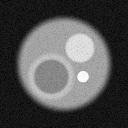
\includegraphics[width=0.38\textwidth]{images/r_3sphere_slice}
	\caption{Fatia do volume \quote{Test Spheres}.}
	\label{fig:r_sphere_slice}
\end{figure}

\begin{figure}[h]
	\centering
	\subfigure[Visualização.]
	{
		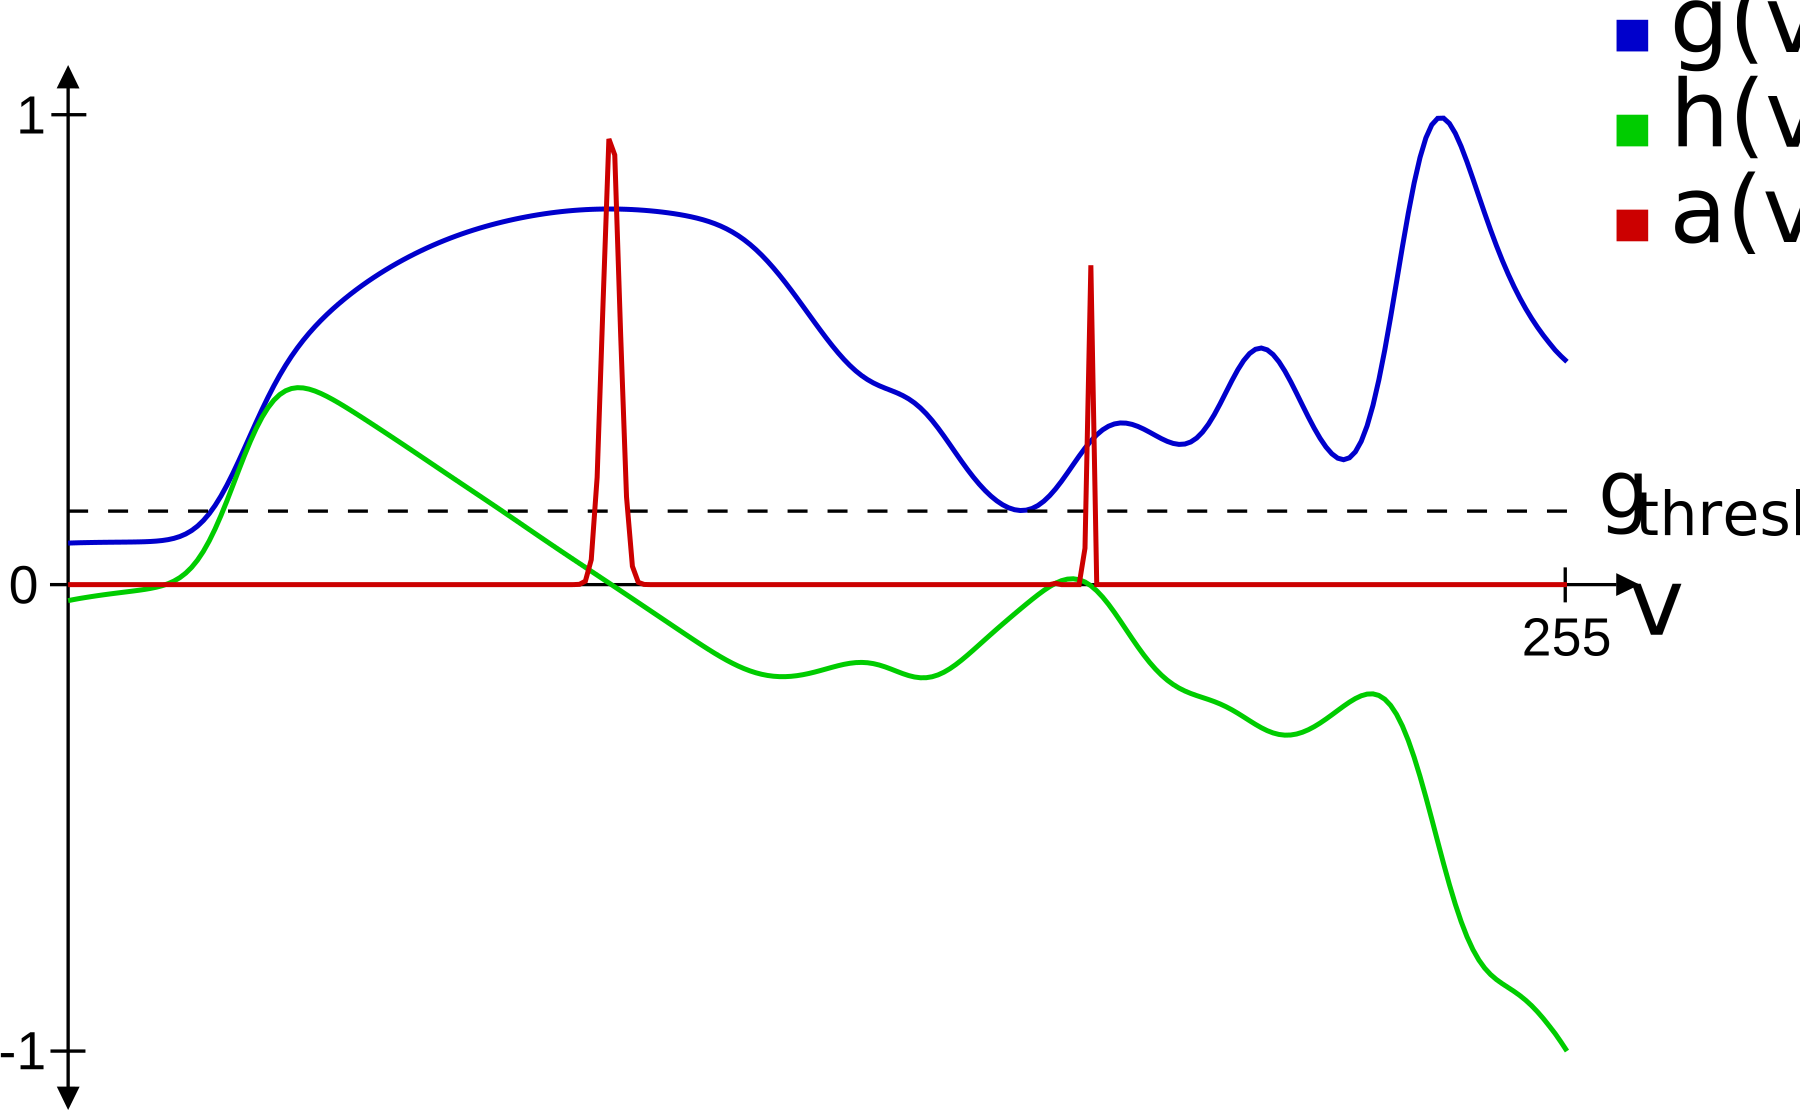
\includegraphics[width=0.3\textwidth]{images/r_g_3sphere}
		\label{fig:r_sphere_kd_vis}
	}
	\subfigure[Função de transferência.]
	{
		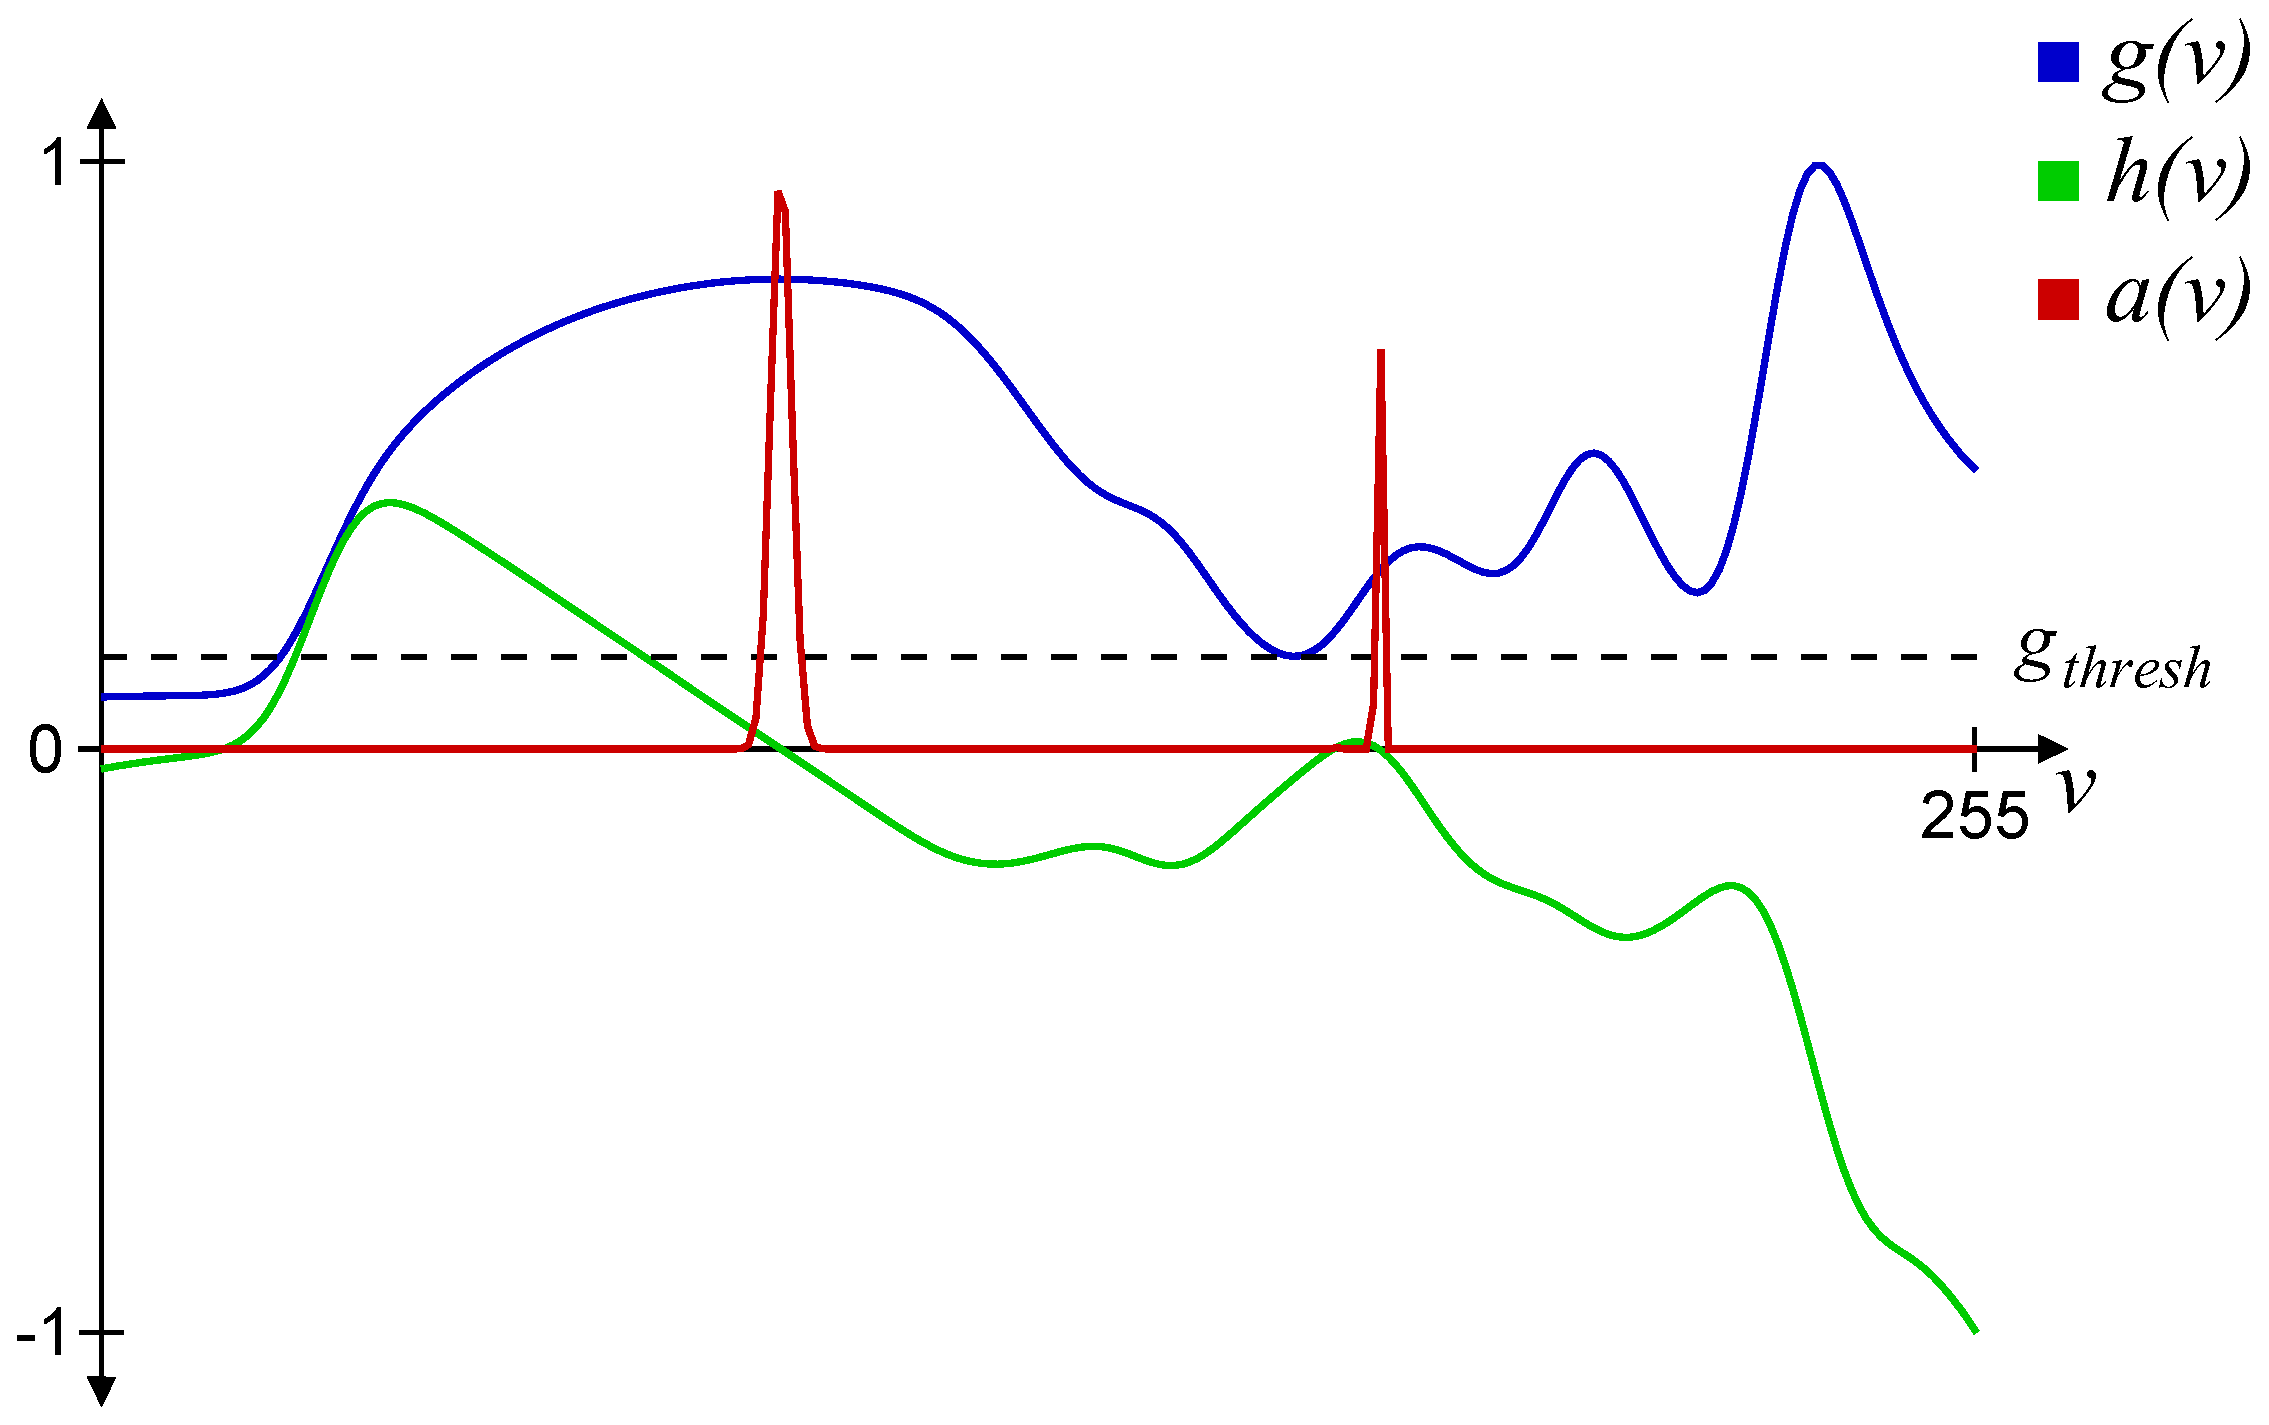
\includegraphics[width=0.65\textwidth]{images/r_g_3sphere_ft}
		\label{fig:r_sphere_kd_ft}
	}
	\caption{Volume \quote{Test Spheres} pelo método de \textit{Kindlmann e Durkin}.}
	\label{fig:r_sphere_kd}
\end{figure}

\begin{figure}[h]
	\centering
	\subfigure[Visualização.]
	{
		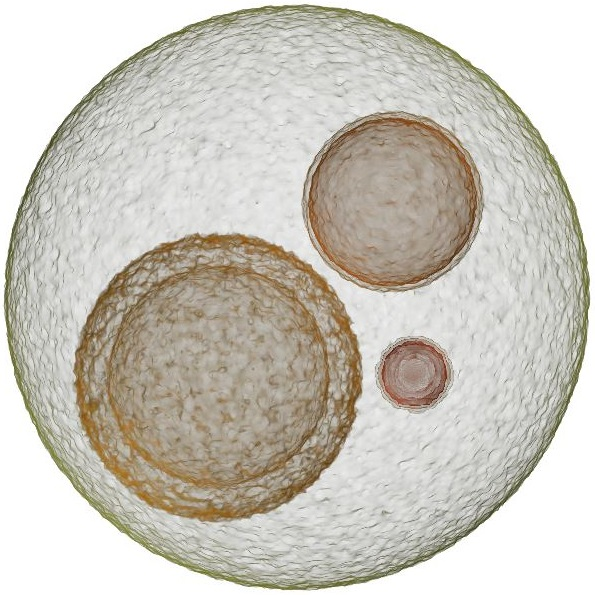
\includegraphics[width=0.3\textwidth]{images/r_m_3sphere}
		\label{fig:r_sphere_mine_vis}
	}
	\subfigure[Função de transferência.]
	{
		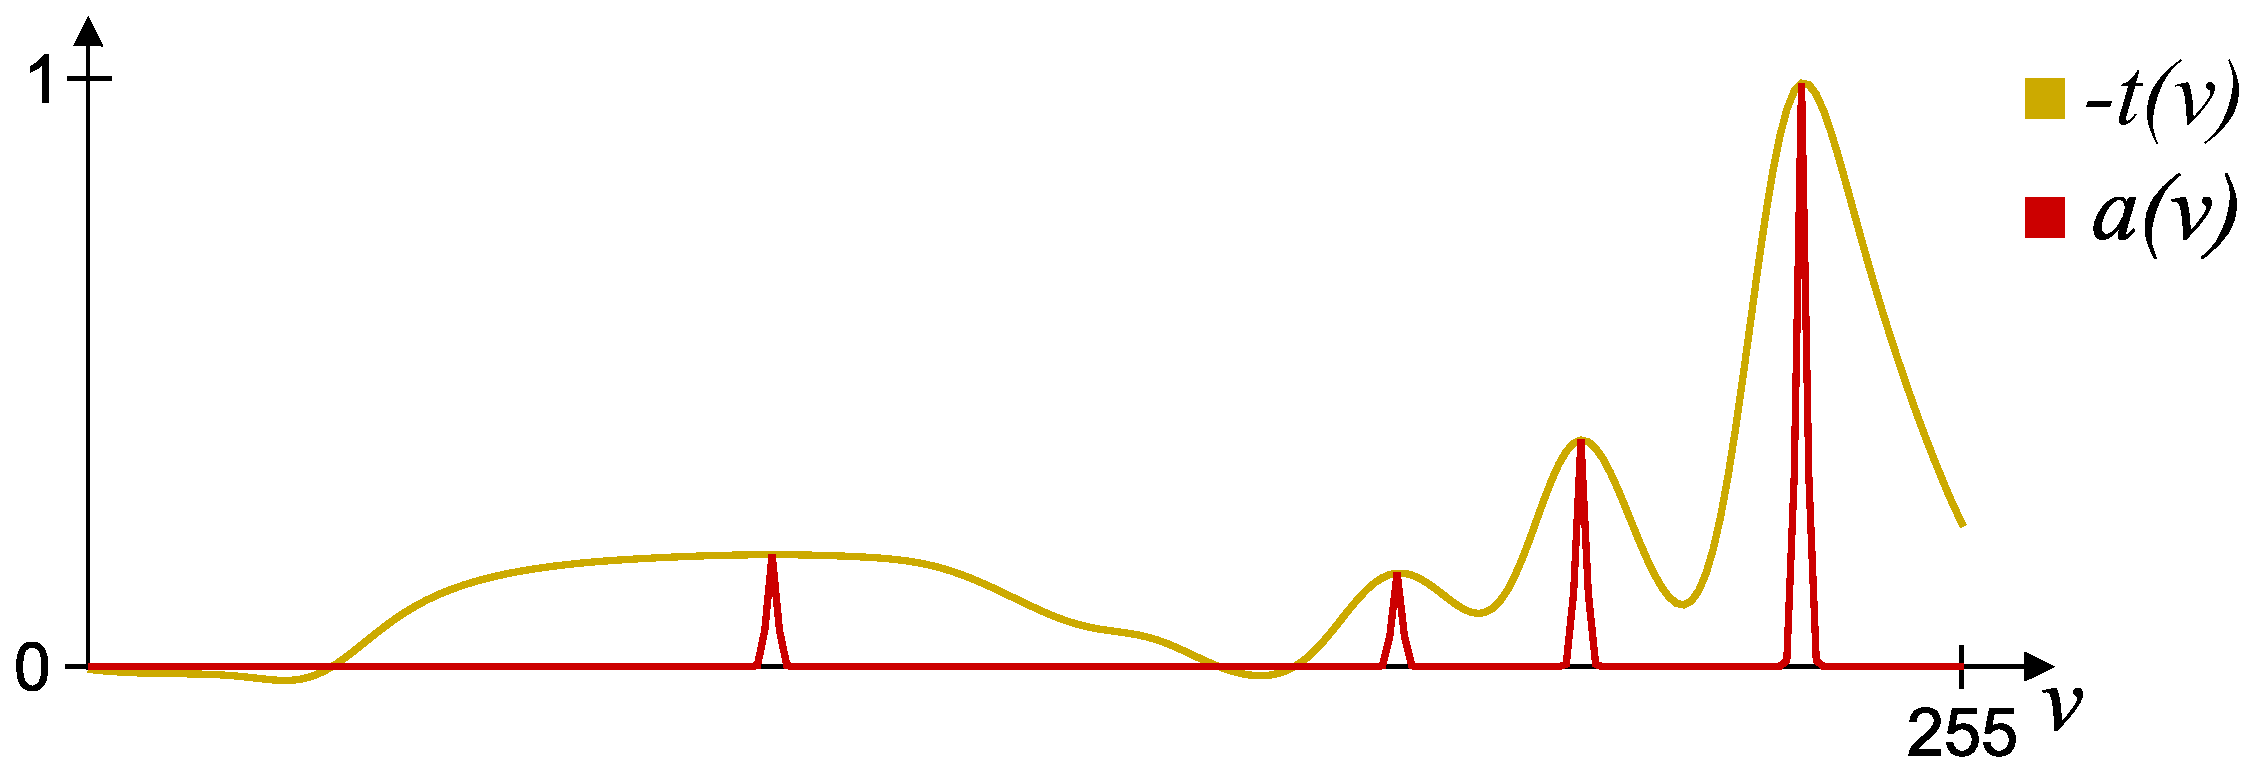
\includegraphics[width=0.65\textwidth]{images/r_m_3sphere_ft}
		\label{fig:r_sphere_mine_ft}
	}
	\caption{Volume \quote{Test Spheres} pelo método proposto.}
	\label{fig:r_sphere_mine}
\end{figure}

%%%%%%%%%%%%%%%%%%%%%%%%%%%%%%%%%% NUCLEON %%%%%%%%%%%%%%%%%%%%%%%%%%%%%%%%%%%%%
\newpage
	A Figura~\ref{fig:r_nucleon_slice} mostra uma fatia do volume \quote{Nucleon}. Nela é possível observar duas fronteiras: preto-cinza, cinza-branco. A Figura~\ref{fig:r_nucleon_kd}~\ref{fig:r_nucleon_kd_ft} mostra que o método de \textit{Kindlmann e Durkin} identifica apenas uma fronteira, enquanto o método proposto por esta dissertação identifica as duas existentes, como mostra a Figura~\ref{fig:r_nucleon_mine}~\ref{fig:r_nucleon_mine_ft}.
	
	A fronteira mais externa do volume foi identificada pelos dois métodos, mas como isosuperfícies diferentes. No entanto, não é possível avaliar qual método identificou o centro correto da fronteira. Como o volume não é sintético, essa análise só poderia ser feita a partir de sua fatia, o que não permite conclusões apropriadas.
	
	É importante ressaltar que o valor escolhido para o $ g_{thresh} $ neste volume não ocasionou a perda da fronteira não detectada. Mesmo com threshold igual a zero, apenas uma fronteira é detectada. Neste caso, o $ g_{thresh} $ foi usado para permitir uma fronteira mais fina.
	
\begin{figure}[h]
	\centering
	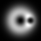
\includegraphics[width=0.33\textwidth]{images/g_nucleon_slice}
	\caption{Fatia do volume \quote{Nucleon}.}
	\label{fig:r_nucleon_slice}
\end{figure}

\begin{figure}[h]
	\centering
	\subfigure[Visualização.]
	{
		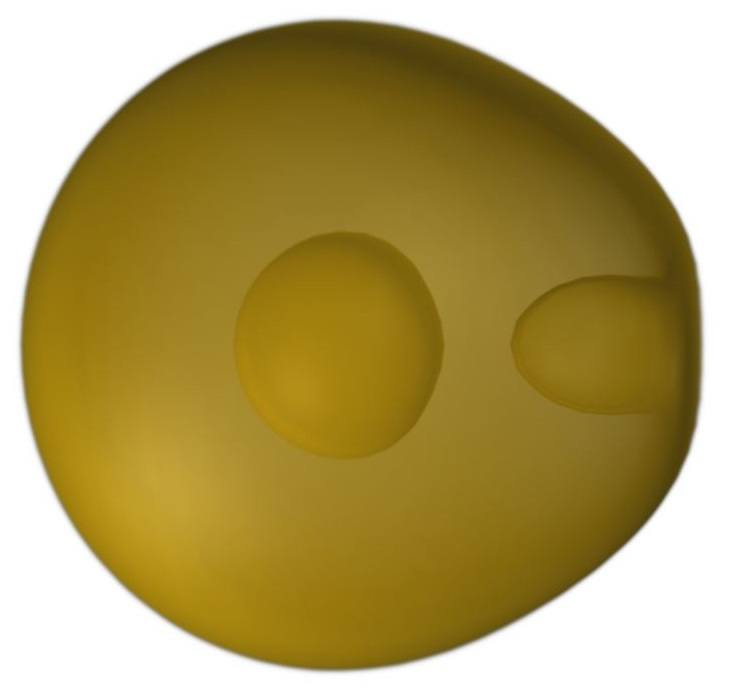
\includegraphics[width=0.3\textwidth]{images/g_nucleon}
		\label{fig:r_nucleon_kd_vis}
	}
	\subfigure[Função de transferência.]
	{
		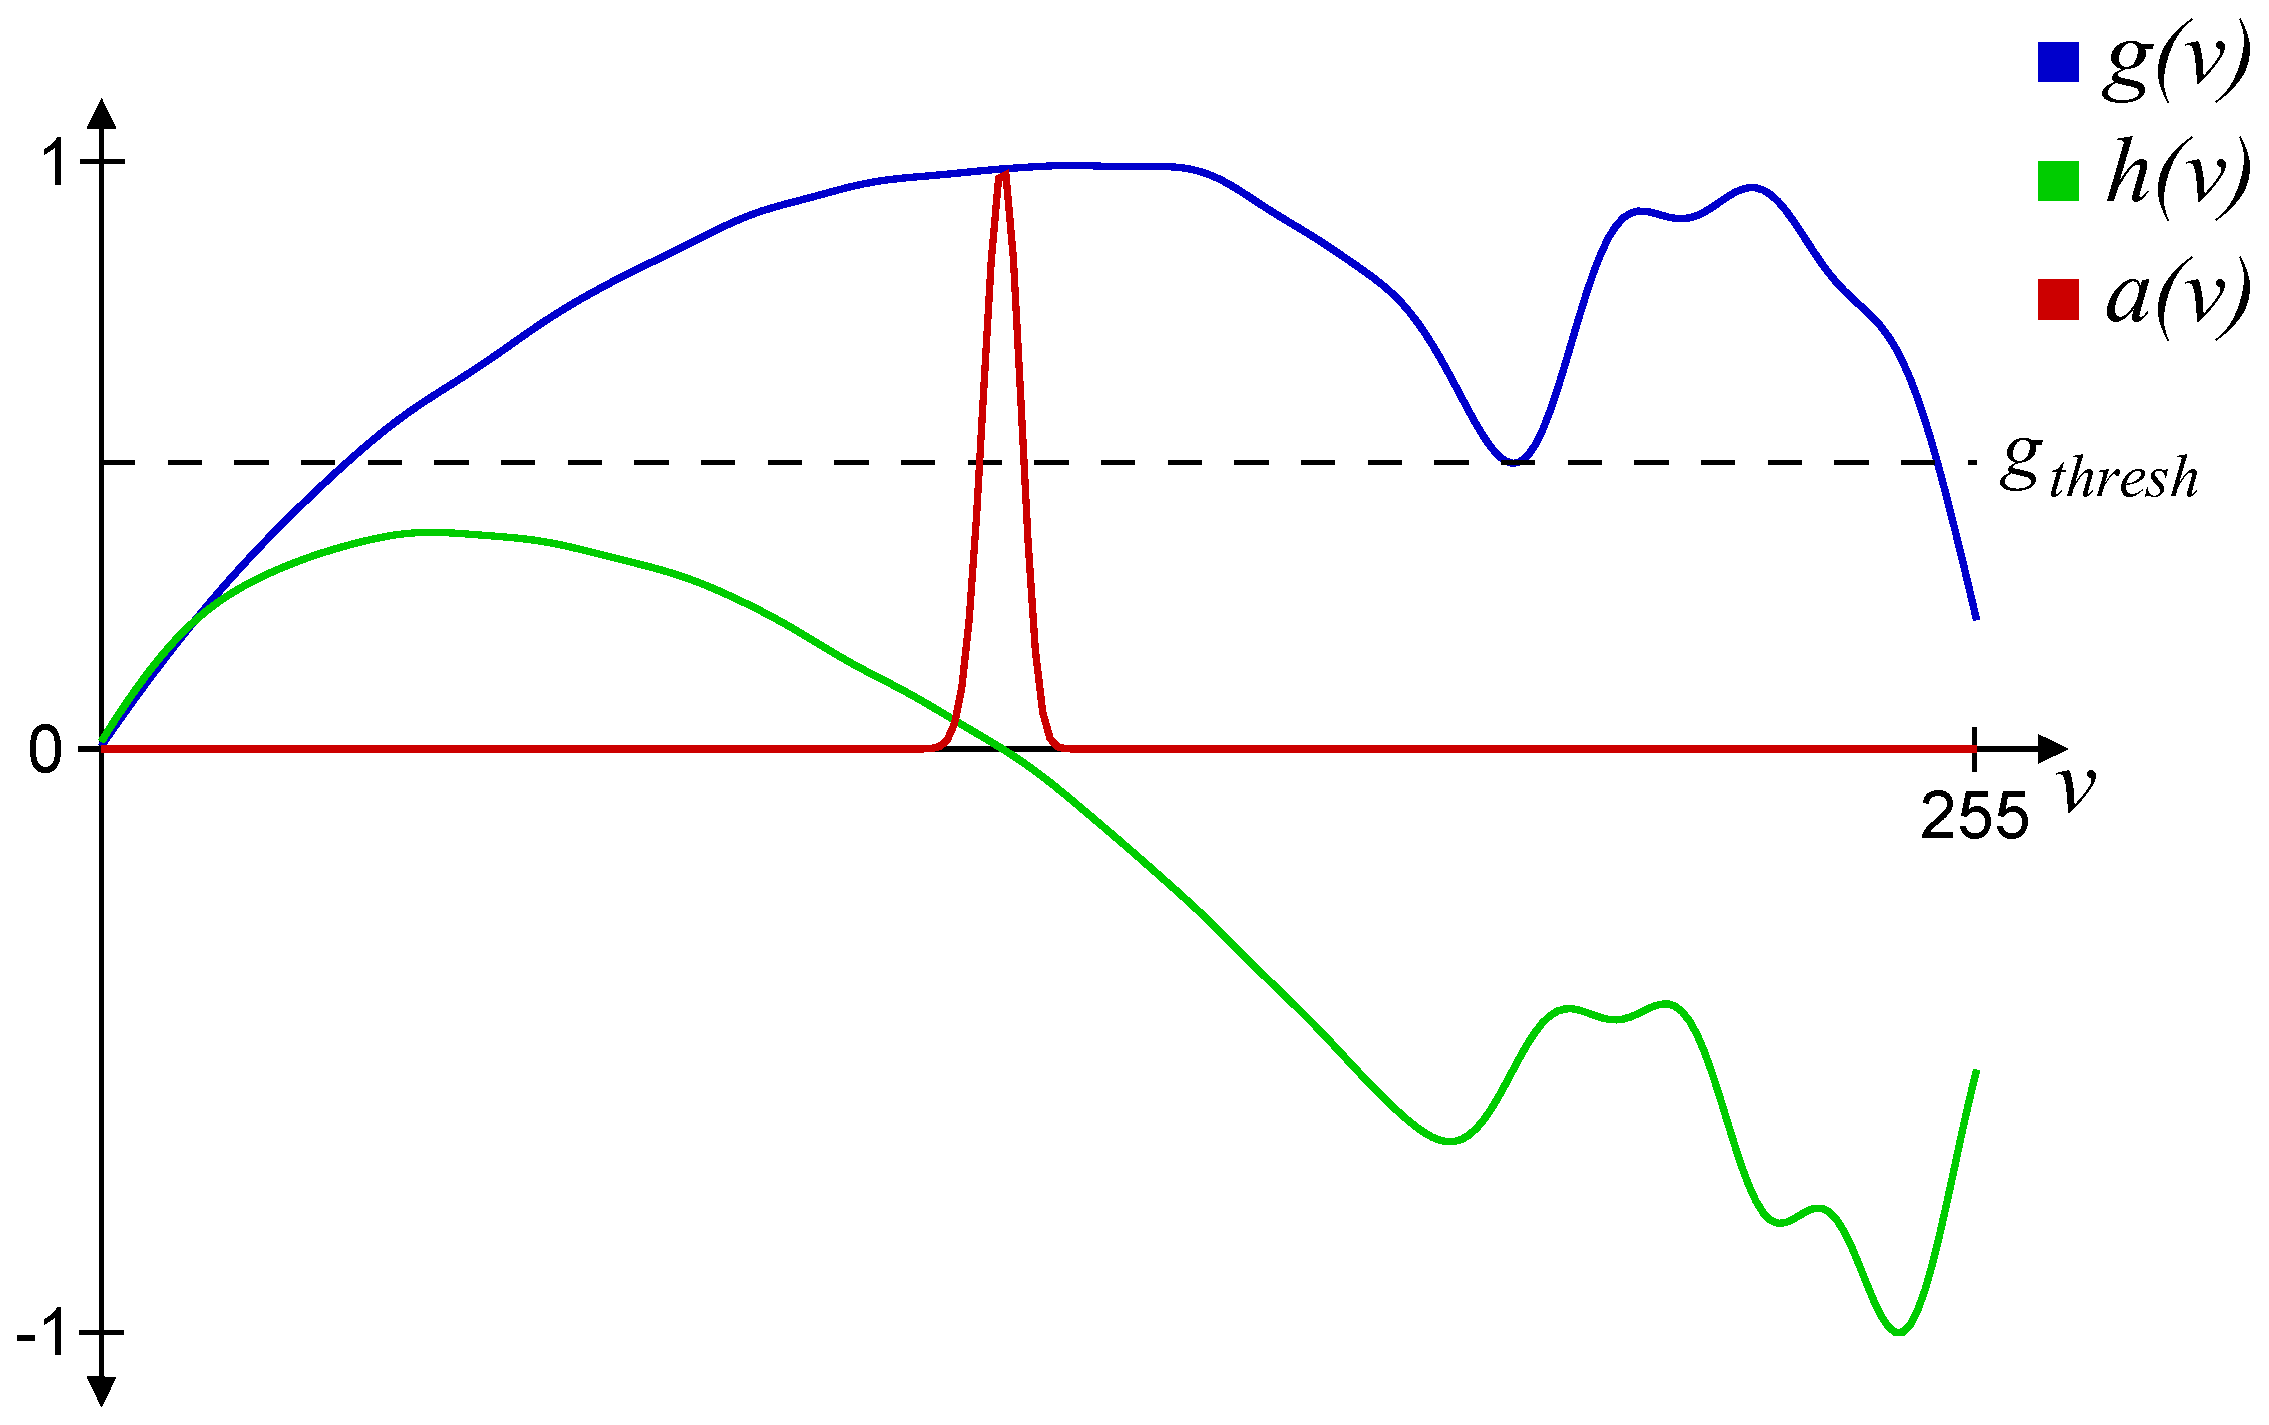
\includegraphics[width=0.65\textwidth]{images/r_g_nucleon_ft}
		\label{fig:r_nucleon_kd_ft}
	}
	\caption{Volume \quote{Nucleon} pelo método de \textit{Kindlmann e Durkin}.}
	\label{fig:r_nucleon_kd}
\end{figure}

\begin{figure}[h]
	\centering
	\subfigure[Visualização.]
	{
		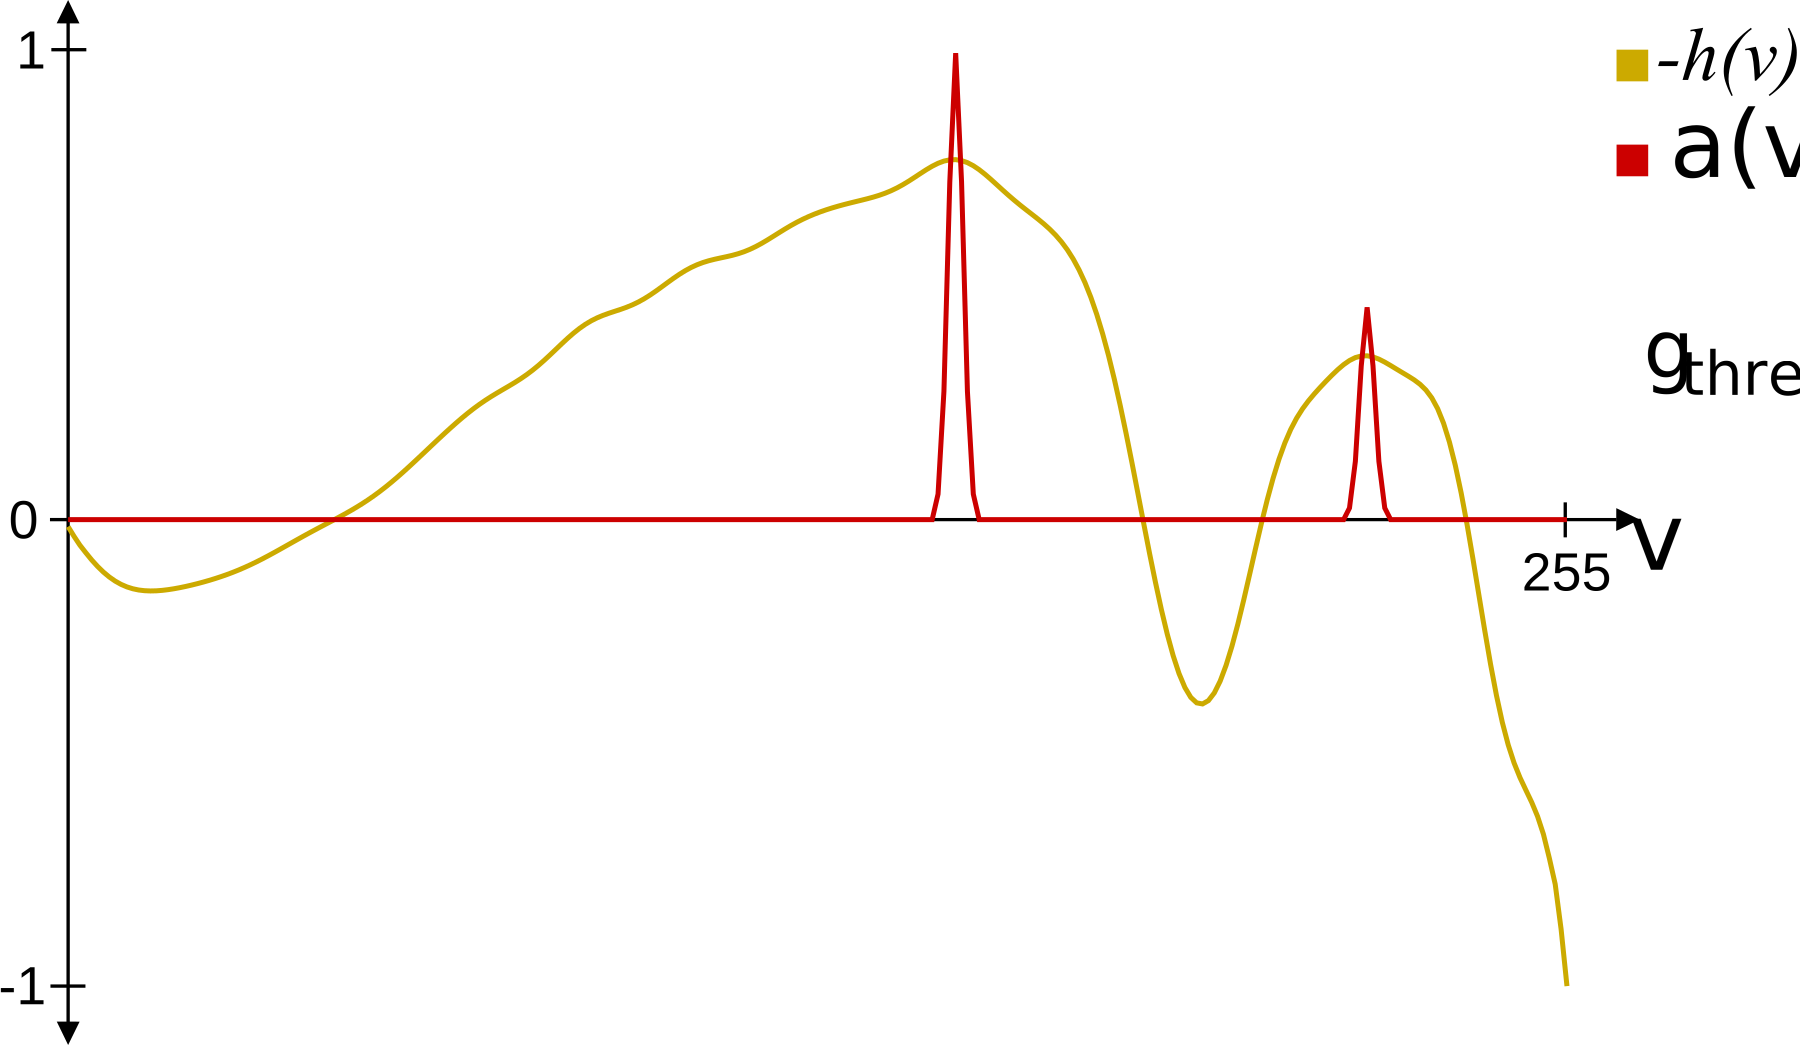
\includegraphics[width=0.3\textwidth]{images/r_m_nucleon}
		\label{fig:r_nucleon_min_vis}
	}
	\subfigure[Função de transferência.]
	{
		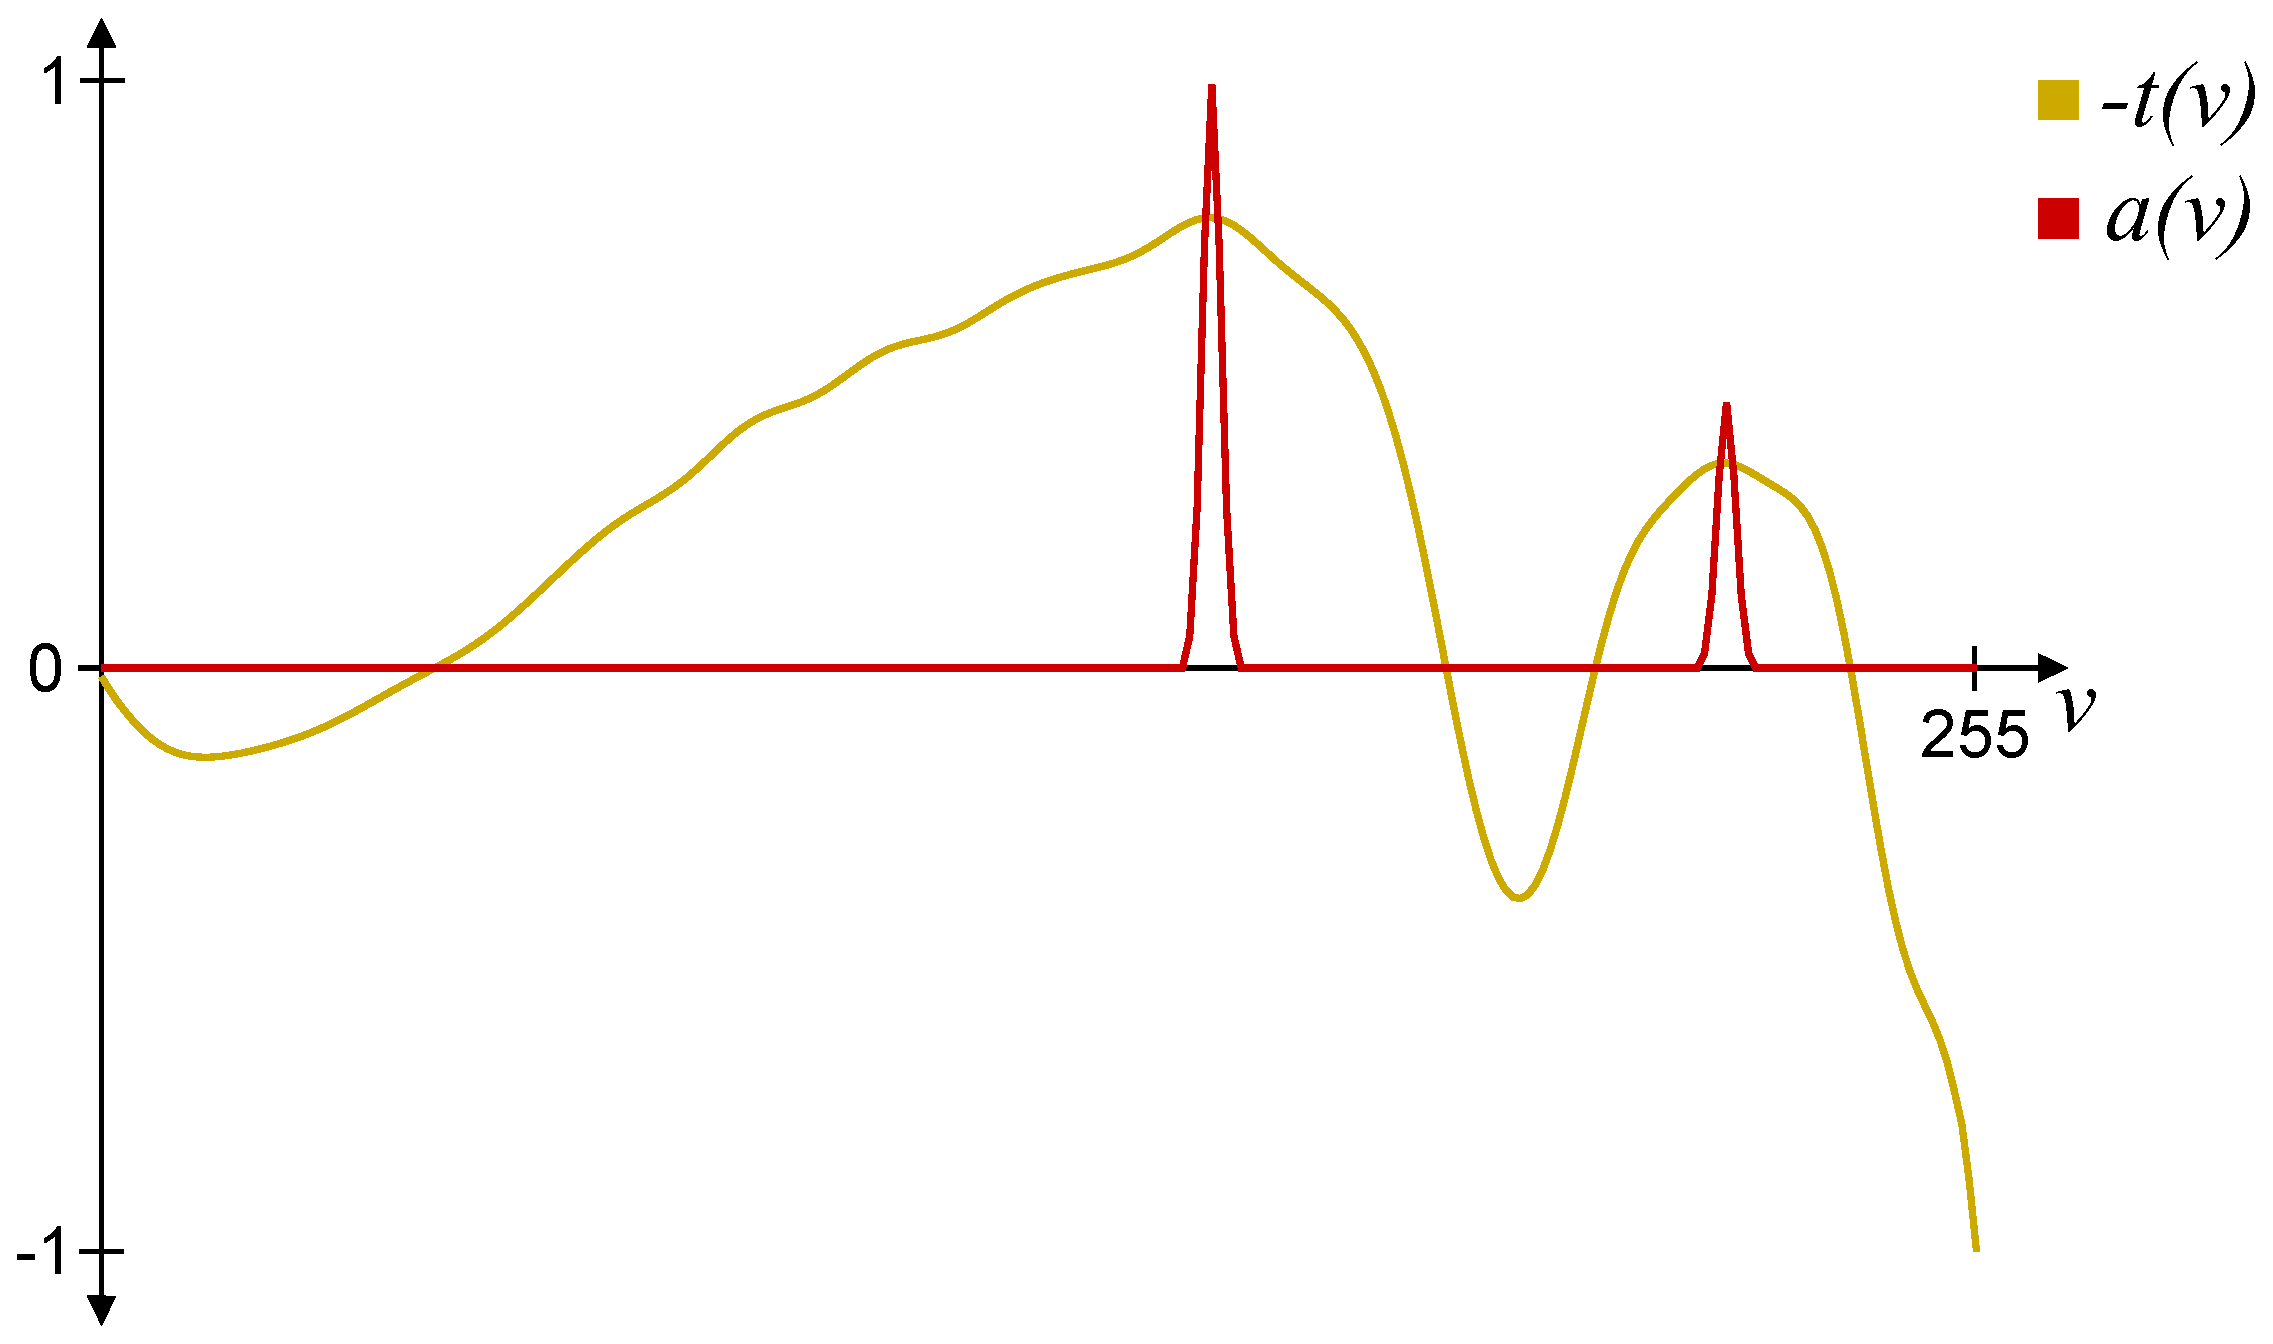
\includegraphics[width=0.65\textwidth]{images/r_m_nucleon_ft}
		\label{fig:r_nucleon_mine_ft}
	}
	\caption{Volume \quote{Nucleon} pelo método proposto.}
	\label{fig:r_nucleon_mine}
\end{figure}
	
%%%%%%%%%%%%%%%%%%%%%%%%%%%%%%%%%% ENGINE %%%%%%%%%%%%%%%%%%%%%%%%%%%%%%%%%%%%%
%	A Figura~\ref{fig:r_engine_slice} exibe uma fatia do volume \quote{Engine}, onde pode ser observada a existência de $ 3 $ fronteiras. Comparando as visualizações resultantes dos dois métodos, exibidas na Figura~\ref{fig:r_engine}, percebe-se que ambos foram capazes de realçar corretamente as fronteiras do volume. No entanto, ressalta-se que esta equivalência só foi possível após encontrar o valor de $ g_{thresh} $ que eliminou algumas regiões da visualização do método de \textit{Kindlmann e Durkin} que foram realçadas indevidamente, devido ao deslocamento do segundo pico da sua função de transferência.
%
%\begin{figure}[h]
%	\centering
%	\subfigure[Método de \textit{Kindlmann e Durkin}.]
%	{
%		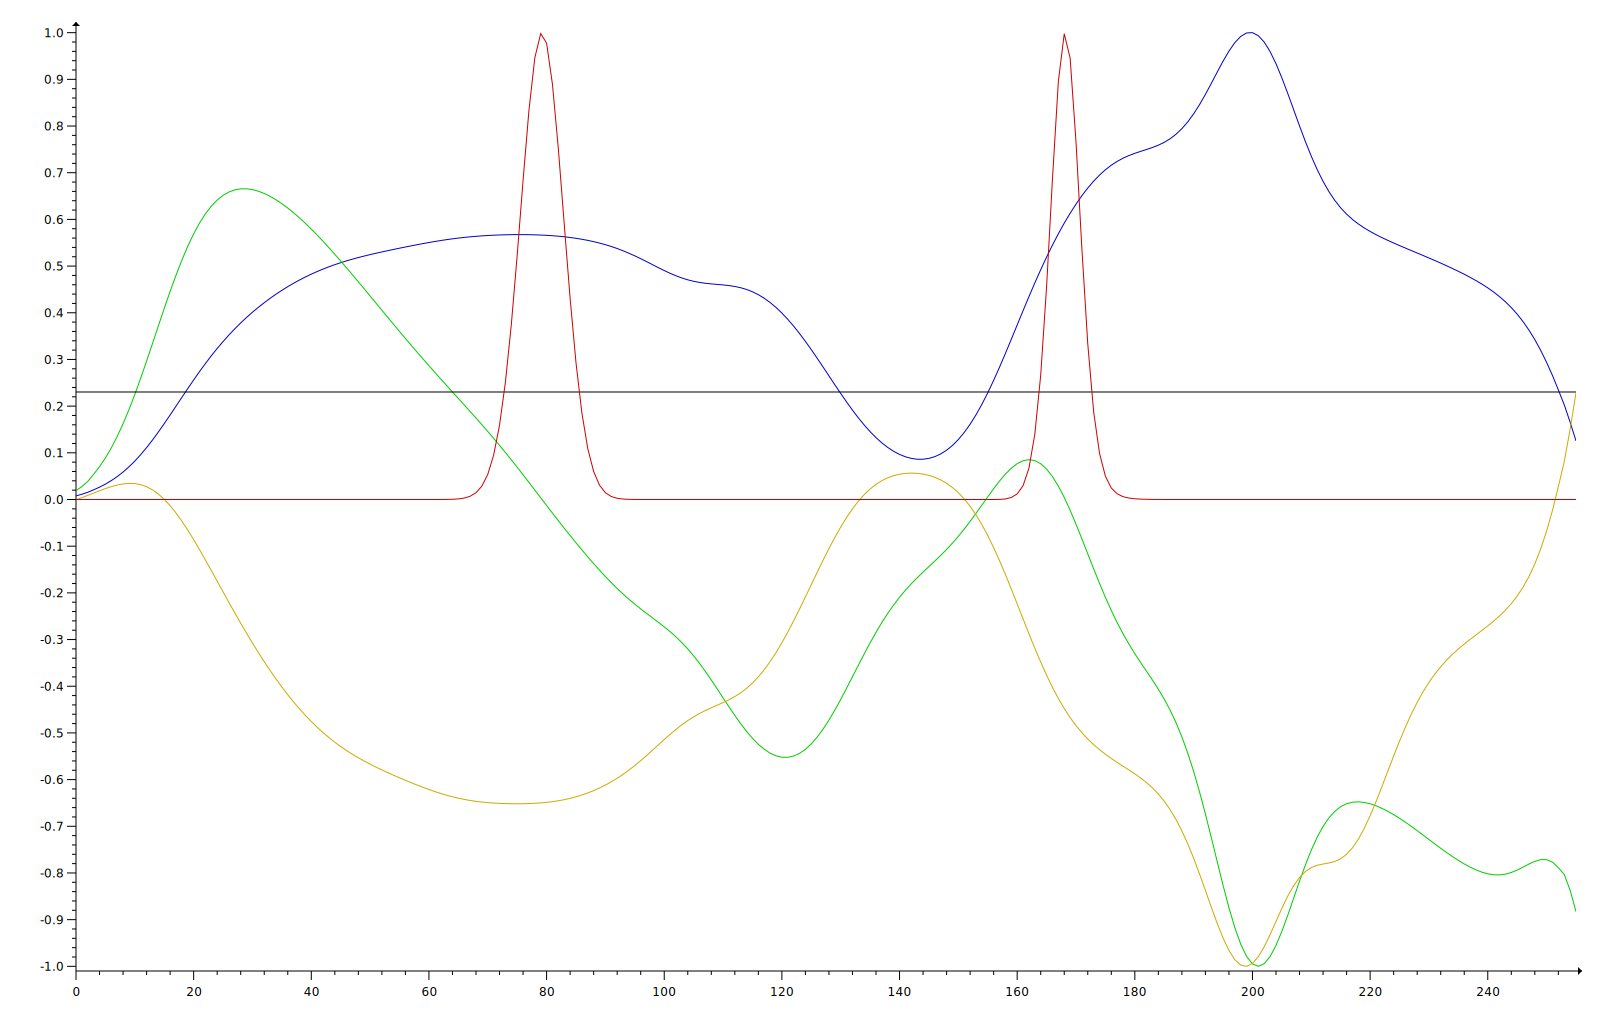
\includegraphics[width=0.35\textwidth]{images/r_g_engine}
%		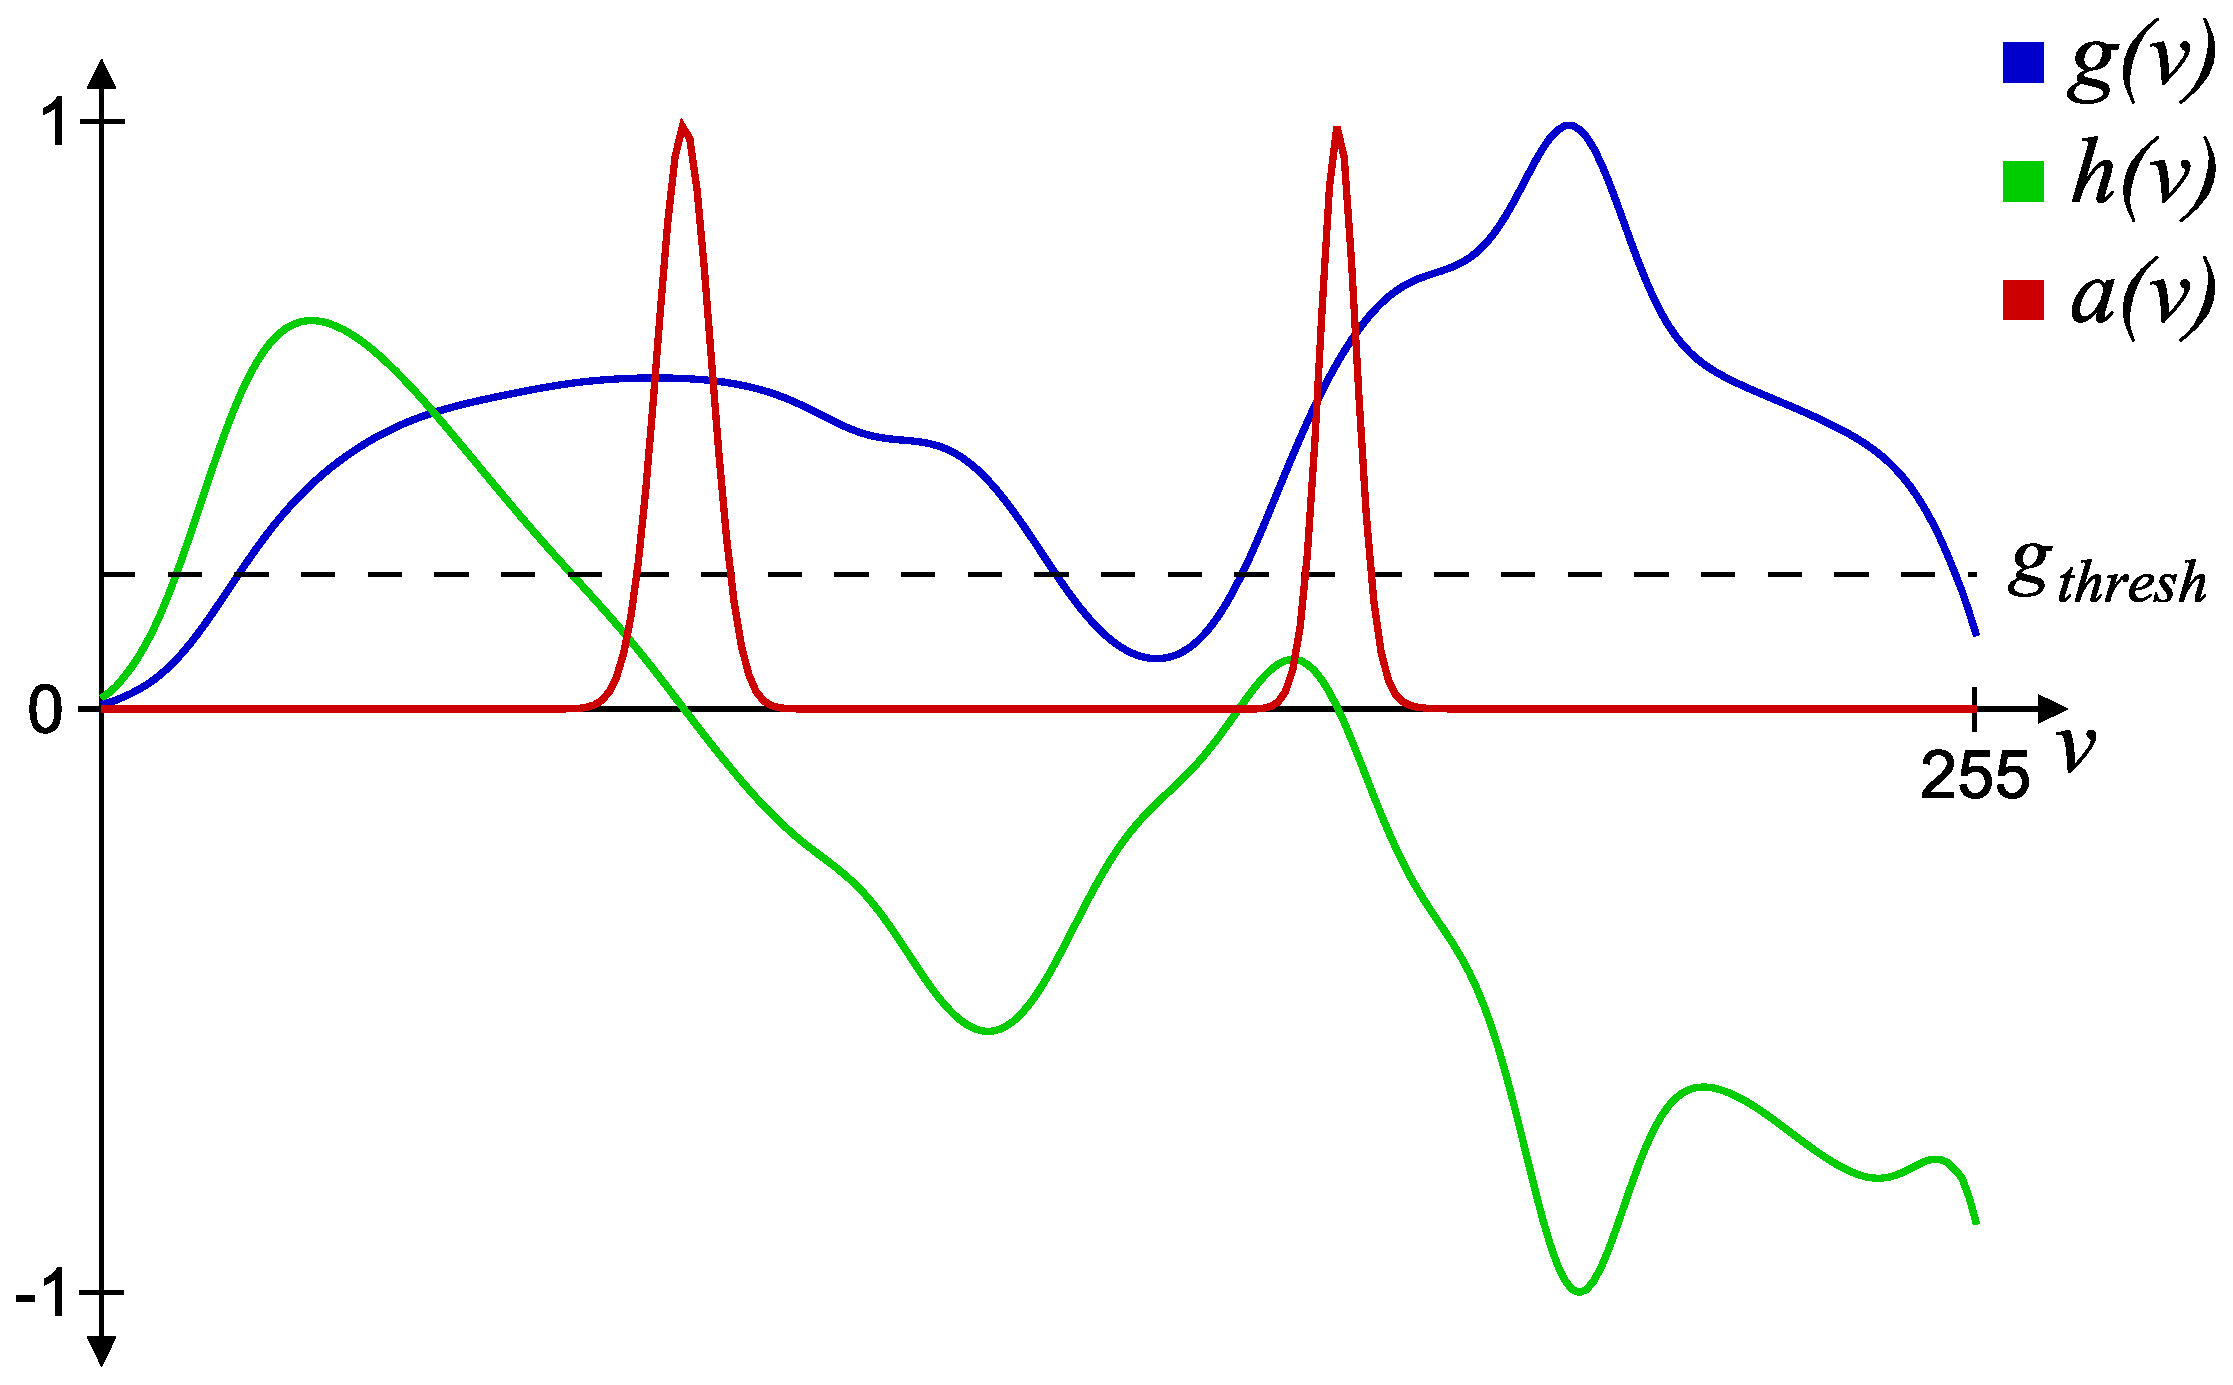
\includegraphics[width=0.65\textwidth]{images/r_g_engine_ft}
%		\label{fig:r_engine_kd}
%	}
%	\subfigure[Método proposto.]
%	{
%		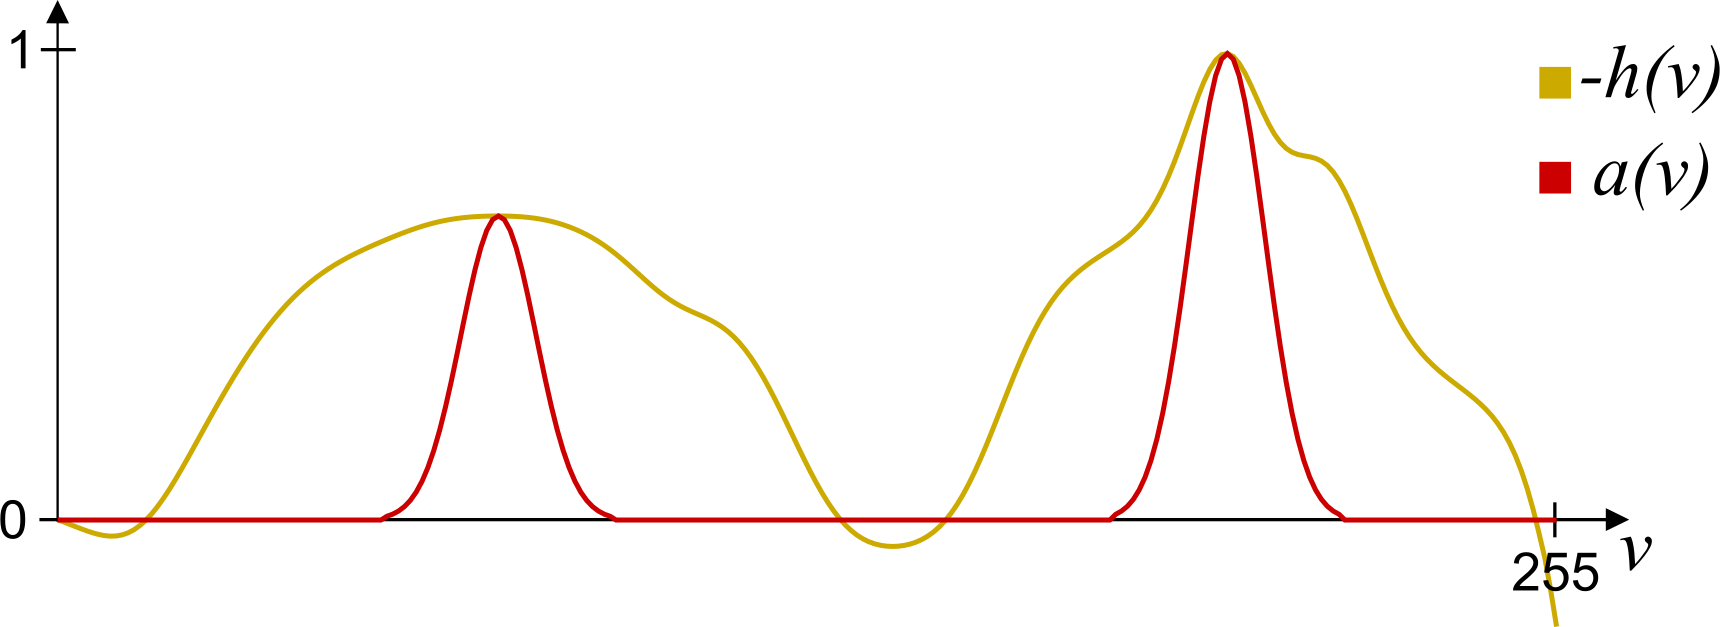
\includegraphics[width=0.35\textwidth]{images/r_m_engine}
%		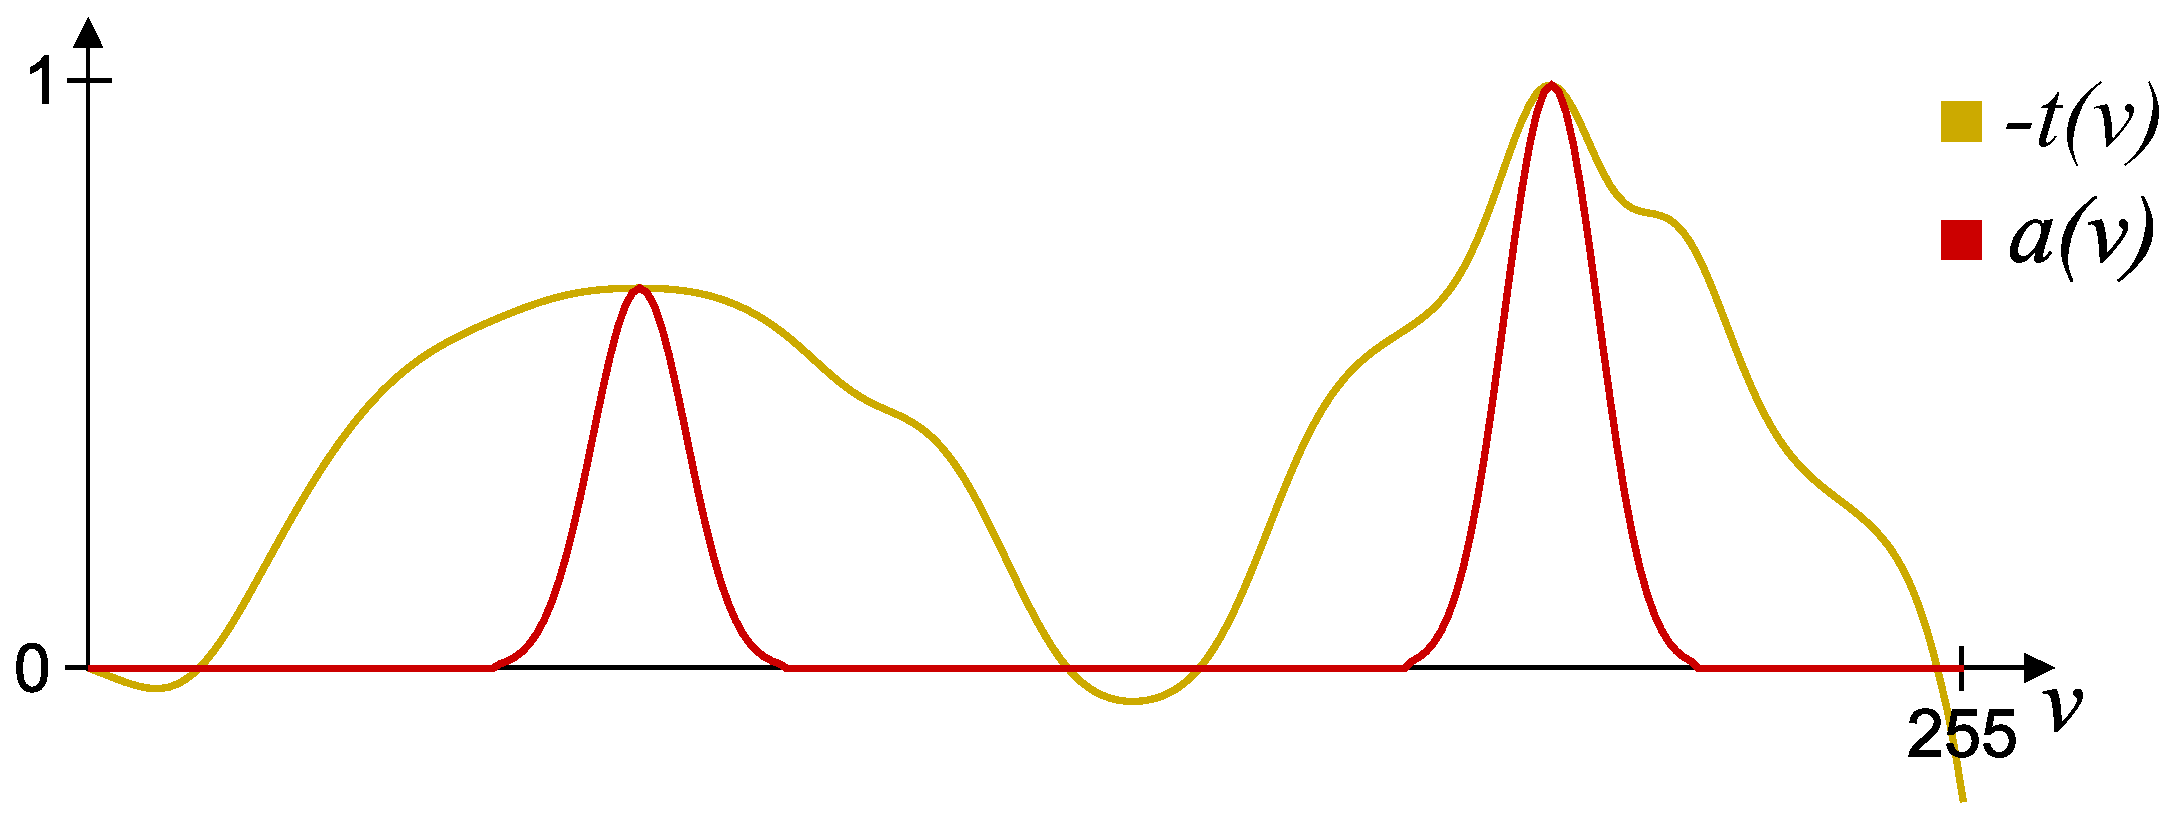
\includegraphics[width=0.65\textwidth]{images/r_m_engine_ft}			\label{fig:r_engine_mine}
%	}
%	\caption{Visualização e função de transferência do volume \quote{Engine}.}
%	\label{fig:r_engine}
%\end{figure}
%%%%%%%%%%%%%%%%%%%%%%%%%%%%%%%%%% CT HEAD %%%%%%%%%%%%%%%%%%%%%%%%%%%%%%%%%%%%%
\newpage
	O volume a seguir é uma tomografia computadorizada de uma cabeça com uma estrutura de suporte na parte de trás. A Figura~\ref{fig:r_cthead} mostra que os dois métodos realçam a cabeça, o crânio e a estrutura de suporte. O segundo pico das duas funções de transferência são coincidentes e equivalem ao crânio, em amarelo. No entanto, o primeiro pico dos dois métodos não coincidem um com o outro.
	
	O método de \textit{Kindlmann~e~Durkin} apresenta um deslocamento para a esquerda, centralizando esse pico onde a segunda derivada é igual a zero. Devido à posição desse pico, alguns voxels do volume são realçados juntamente com a cabeça e sua estrutura de suporte, permitindo a interpretação de que todos compõem uma só isosuperfície. O mesmo não ocorre com o método proposto por esta dissertação, que realça a cabeça corretamente ao mesmo tempo que mostra menos a estrutura presente na sua parte de trás, permitindo entendê-las como isosuperfícies diferentes.

\begin{figure}[h]
	\centering
	\subfigure[Método de \textit{Kindlmann e Durkin}.]
	{
		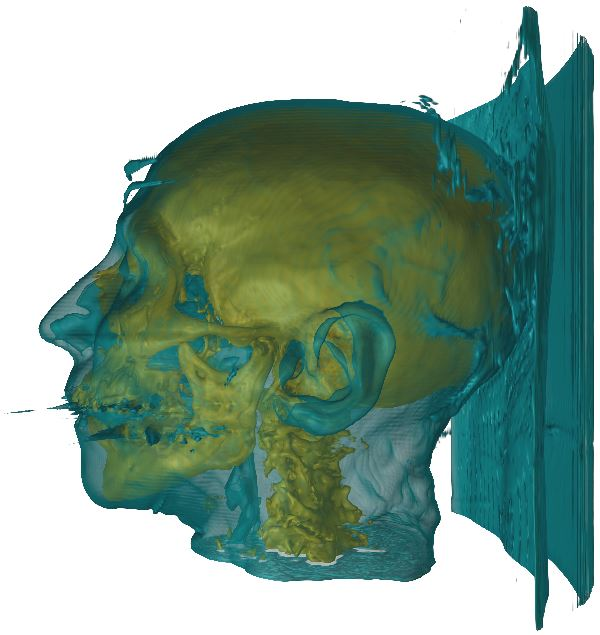
\includegraphics[width=0.35\textwidth]{images/r_g_cthead}
		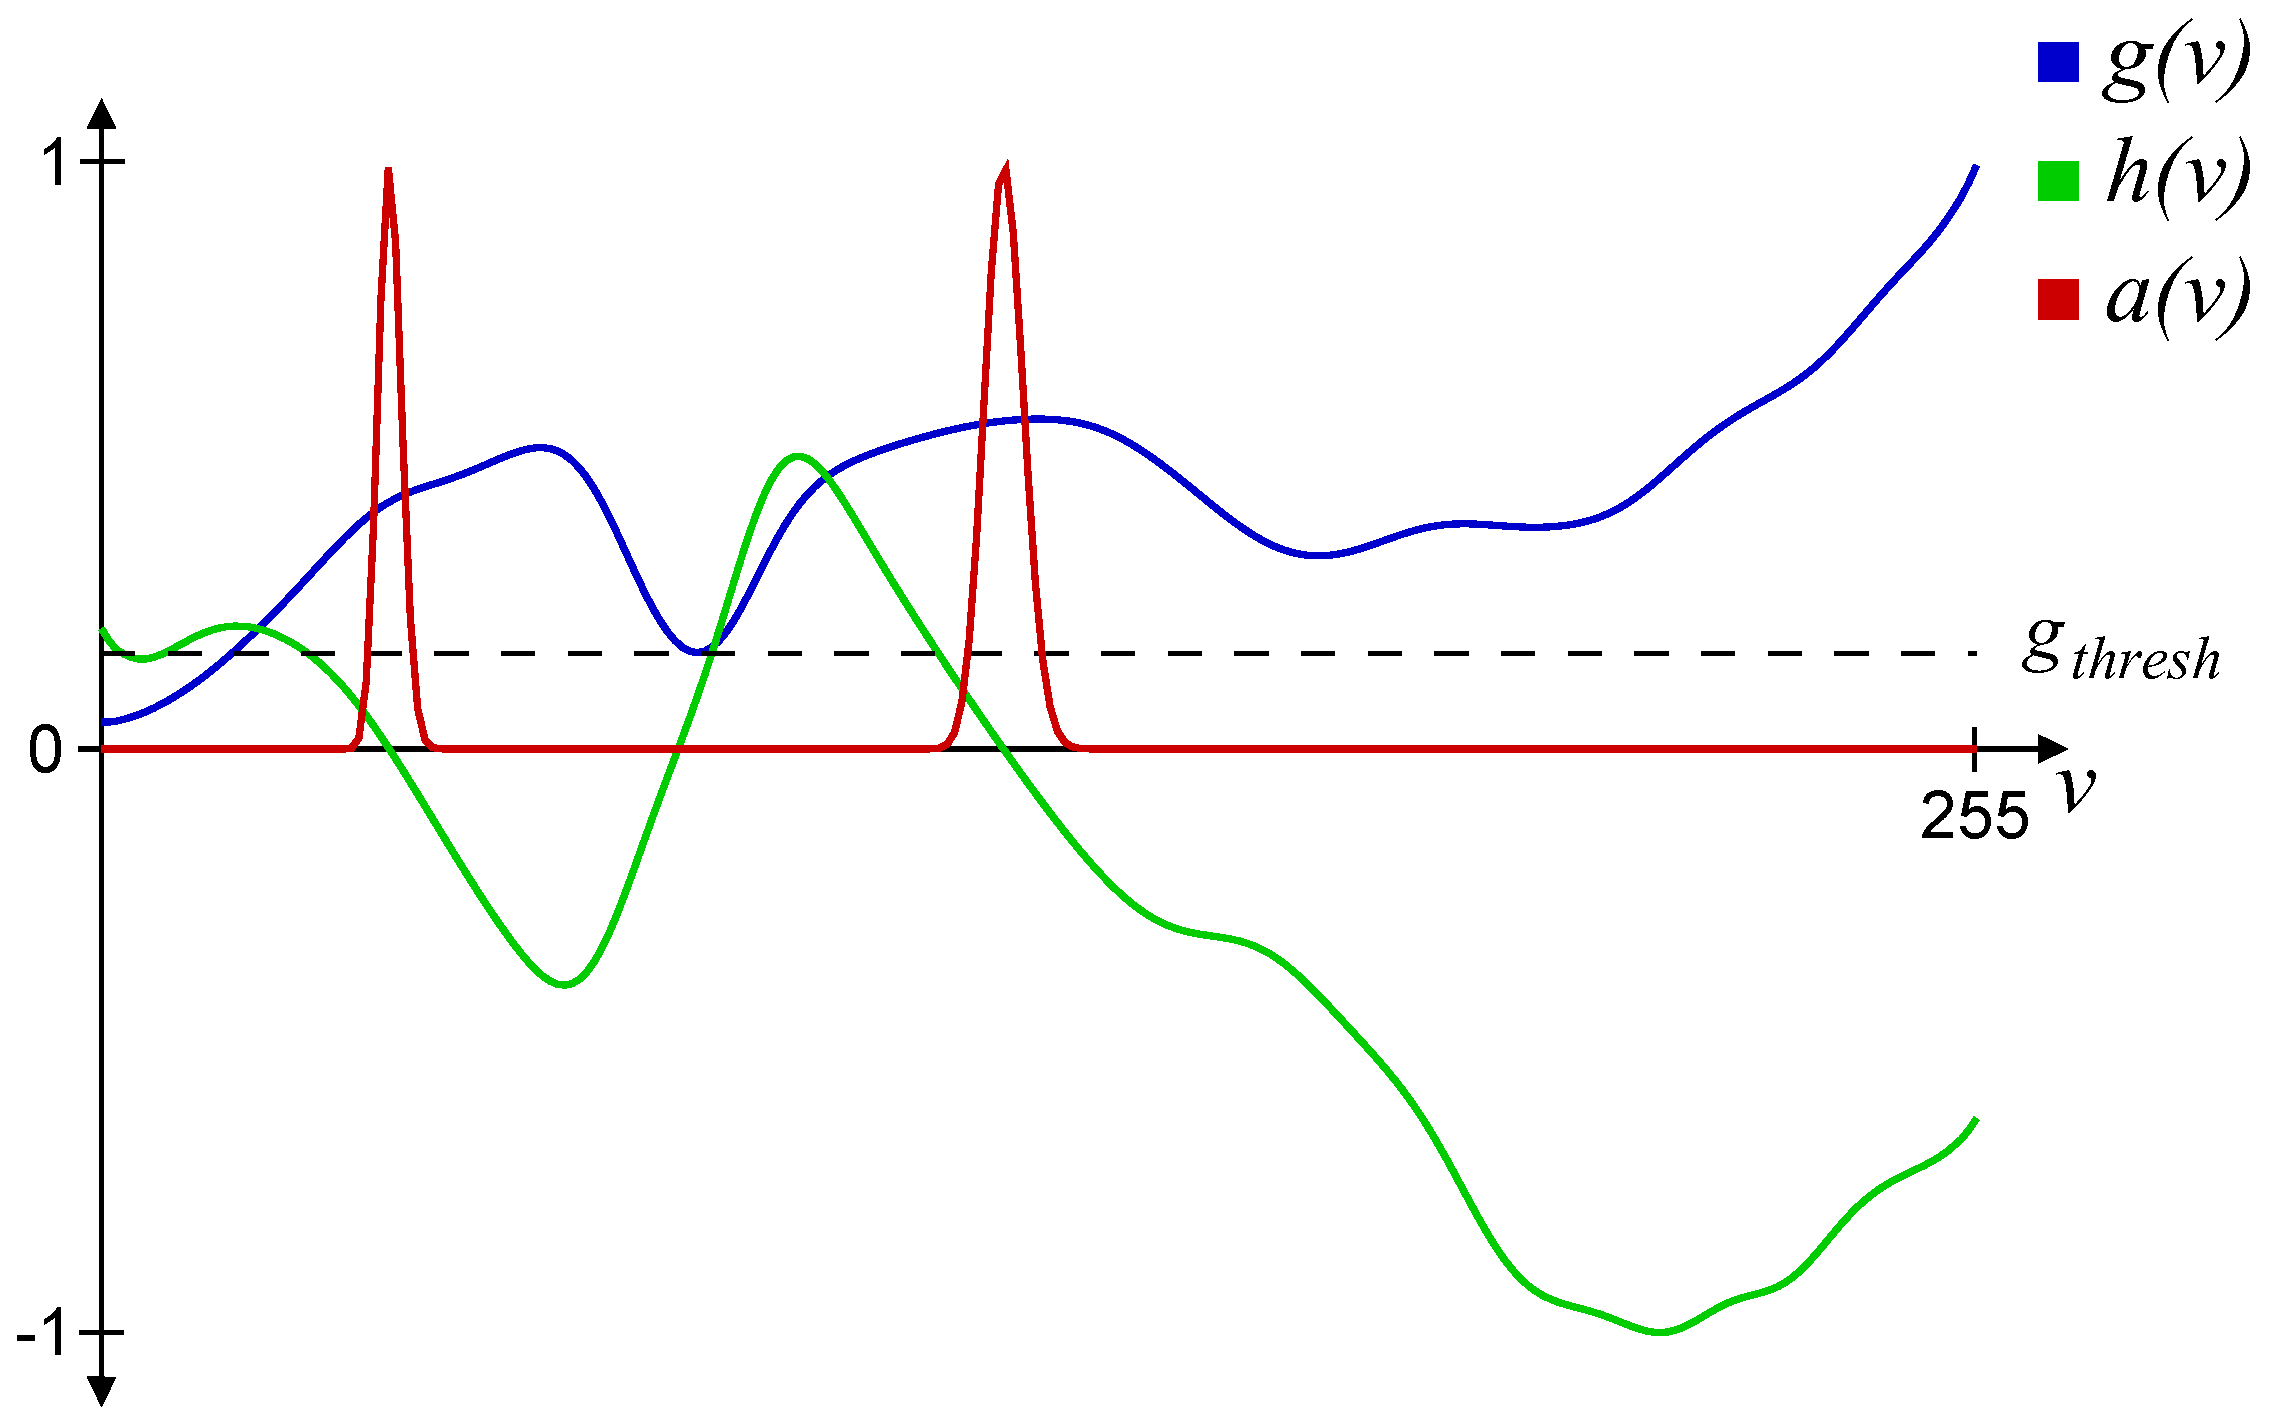
\includegraphics[width=0.65\textwidth]{images/r_g_cthead_ft}
		\label{fig:r_cthead_kd}
	}
	\subfigure[Método proposto.]
	{
		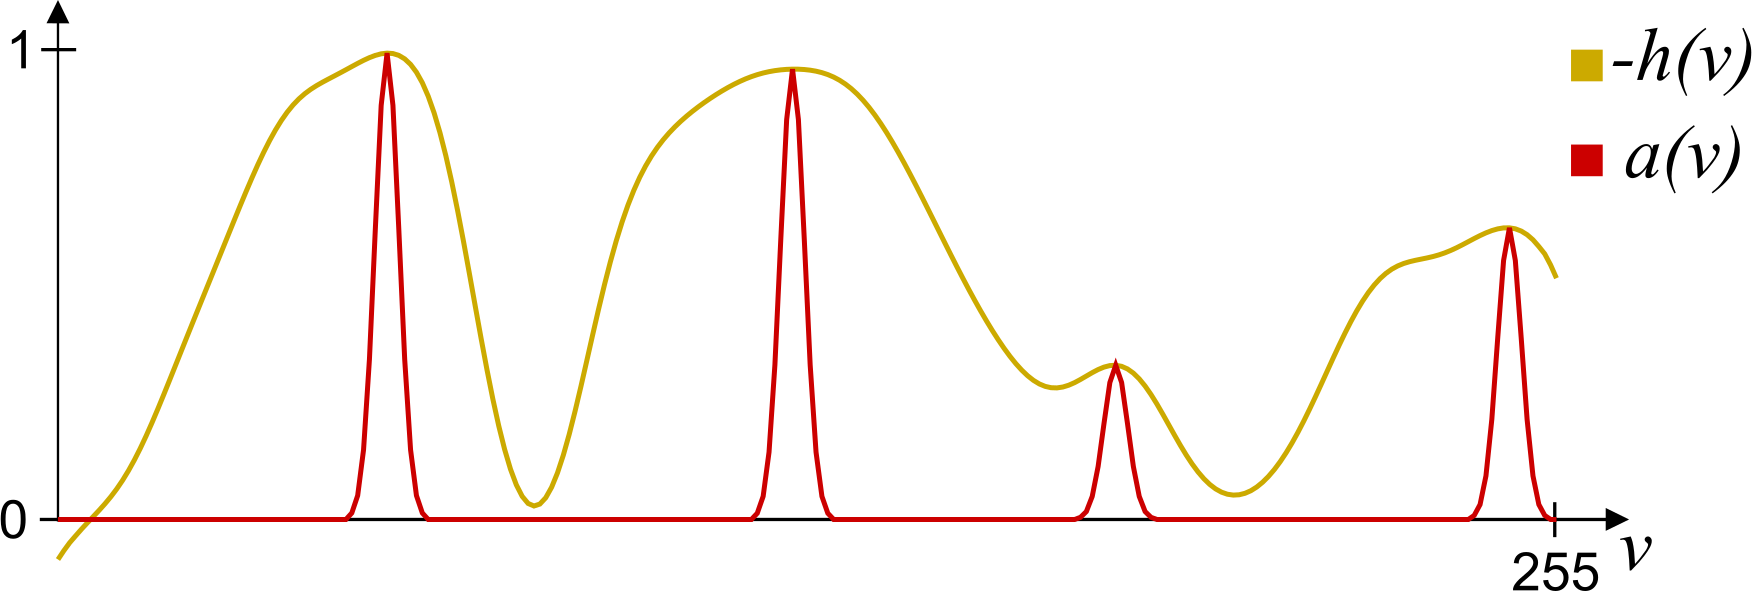
\includegraphics[width=0.35\textwidth]{images/r_m_cthead}
		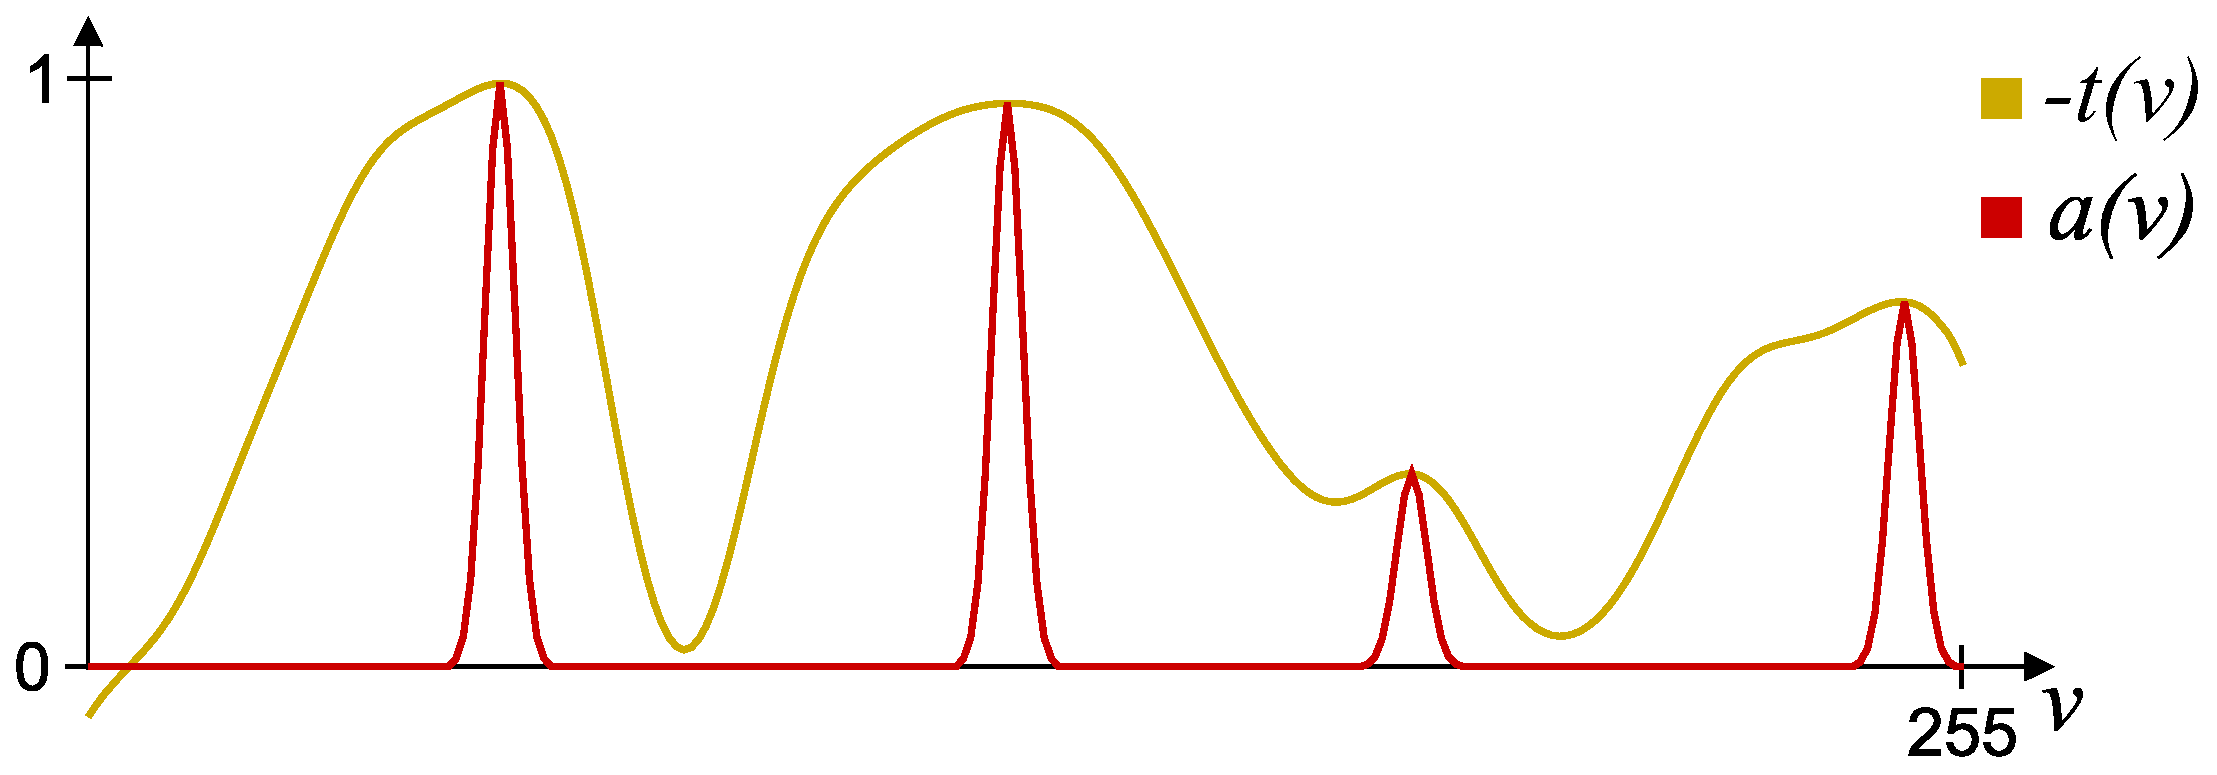
\includegraphics[width=0.65\textwidth]{images/r_m_cthead_ft}			\label{fig:r_cthead_mine}
	}
	\caption{Visualização e função de transferência do volume \quote{CT Head}.}
	\label{fig:r_cthead}
\end{figure}

	A terceira e a quarta fronteira da Figura~\ref{fig:r_cthead}~\ref{fig:r_cthead_mine} realçam regiões de maior intensidades. A terceira é interna ao crânio e a quarta aos dentes. Ambas são vistas separadamente na Figura~\ref{fig:r_cthead_iso2}, respectivamente em laranja e vermelho.
	
\begin{figure}[h]
	\centering
	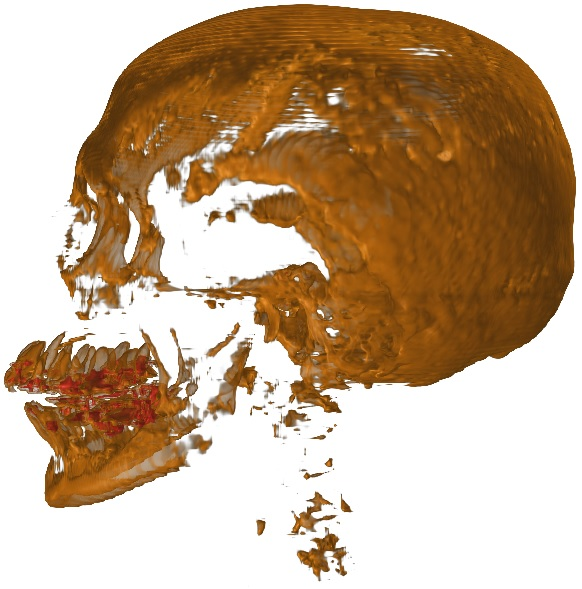
\includegraphics[width=0.5\textwidth]{images/r_m_cthead_iso2}
	\caption{Realce do crânio do volume \quote{CT Head} através da interface.}
	\label{fig:r_cthead_iso2}
\end{figure}
	
	A Figura~\ref{fig:r_cthead_iso} mostra a visualização apenas do crânio, que pode ser obtida através da interface, selecionando apenas a segunda fronteira.

\begin{figure}[h]
	\centering
	\subfigure[Função de transferência.]
	{
		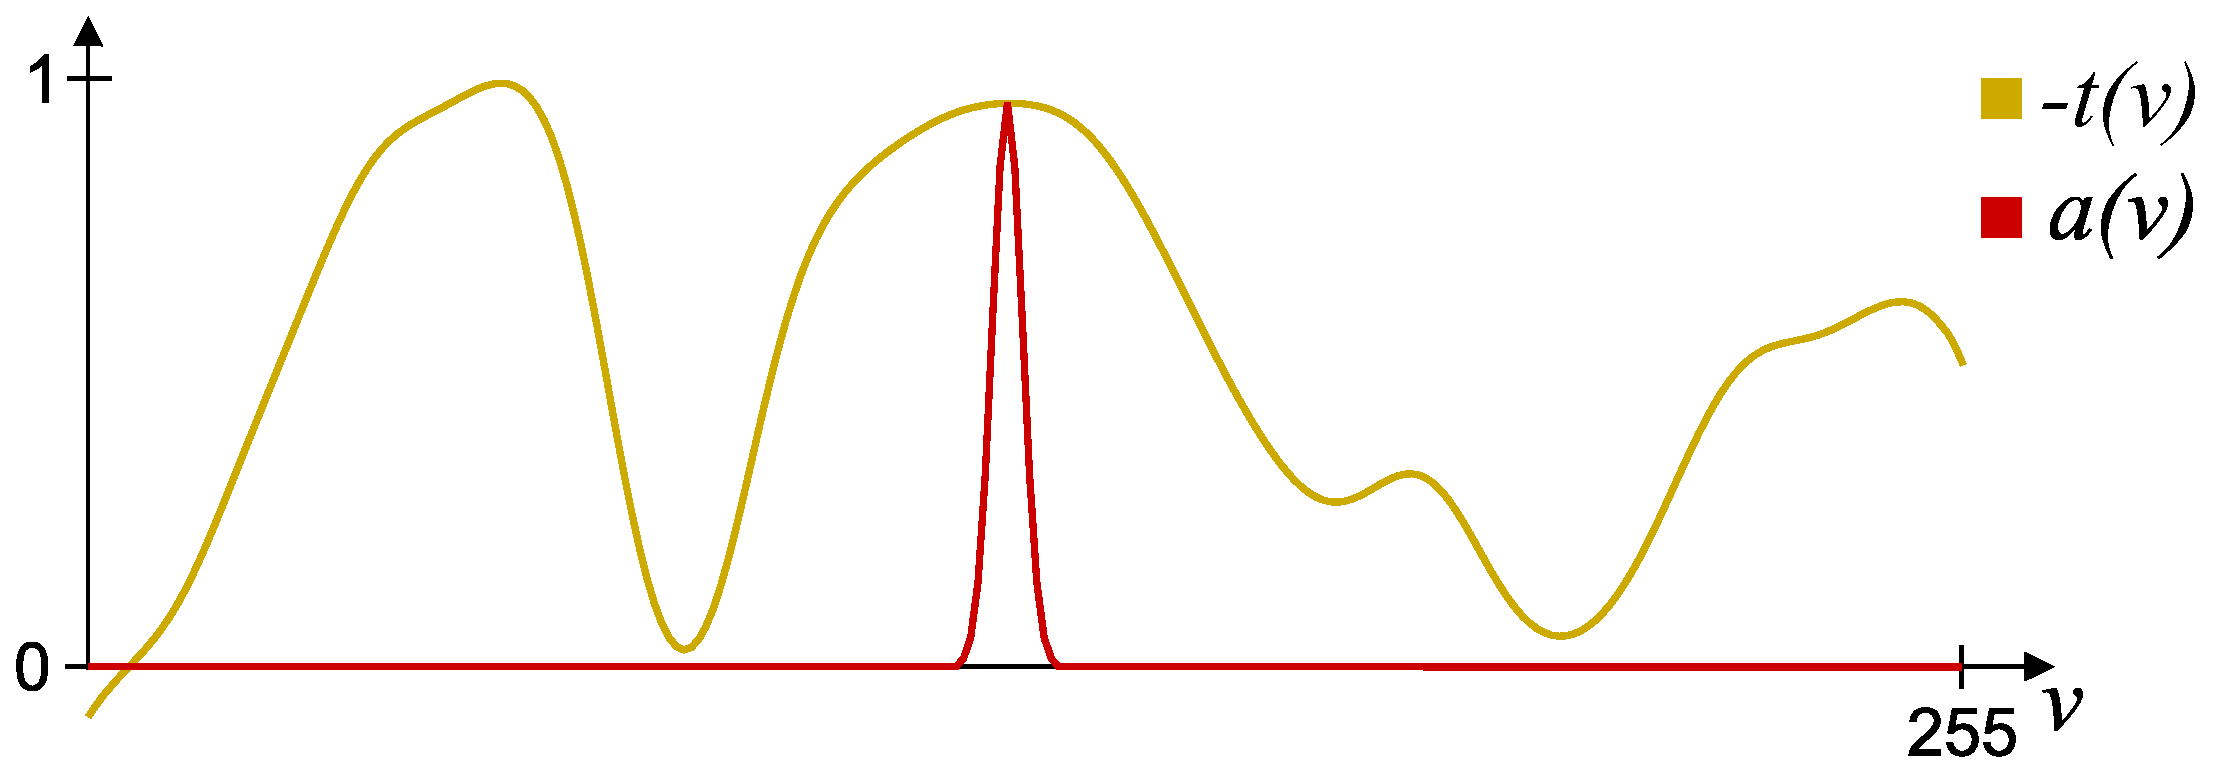
\includegraphics[width=0.8\textwidth]{images/r_m_cthead_iso_ft}
	}
	\subfigure[Visualização volumétrica.]
	{
		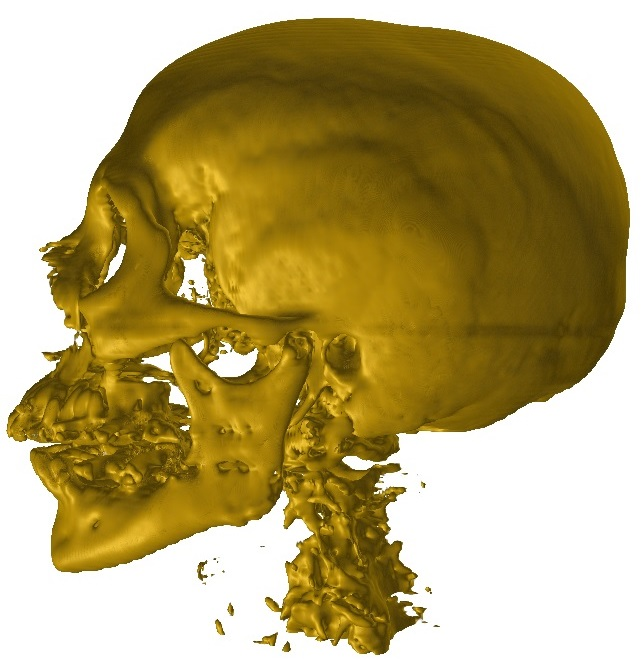
\includegraphics[width=0.7\textwidth]{images/r_m_cthead_iso}
	}
	\caption{Realce do crânio do volume \quote{CT Head} através da interface.}
	\label{fig:r_cthead_iso}
\end{figure}

%%%%%%%%%%%%%%%%%%%%%%%%%%%%%%%%%% Skull %%%%%%%%%%%%%%%%%%%%%%%%%%%%%%%%%%%%%
	As duas últimas fronteiras do volume \quote{CT Head}, identificadas pelo método proposto, são exemplos de fronteiras que não são indicadas pelo máximo local na primeira derivada média. No entanto, essas fronteiras conseguem ser identificadas a partir da terceira, uma vez que seus extremos locais são menos alterados pela média.	A Figura~\ref{fig:r_skull} ilustra melhor essa situação, através do volume \quote{Skull}. Esse volume consiste em apenas um crânio, mas com regiões que contém a mesma intensidade e aparentam ser ruído obtido durante a aquisição dos dados.
	
	Na Figura~\ref{fig:r_skull}, observa-se que o método proposto por esta dissertação realça o crânio com uma quantidade bem menor de ruído, em comparação com o resultado obtido através do método de \textit{Kindlmann e Durkin}. Porém, o mesmo resultado não teria sido obtido se a métrica do método proposto utilizasse máximos locais na primeira derivada média.
	
	Na Figura~\ref{fig:r_skull}~\ref{fig:r_skull_kd} é possível perceber que, próximo à fronteira destacada, encontra-se uma curva acentuada. Este ponto, que pode ser confundido com um máximo local, armazena a maior primeira derivada média da região do crânio. No entanto, esse volume possui uma pequena região de intensidade muito maior que a do crânio, gerando fronteiras mais abruptas e, portanto, de maior derivada.
	
	Essas fronteiras, (que não foram detectadas pelo método de \textit{Kindlmann e Durkin}, apenas pelo método proposto) se sobrepõem com a do crânio. Isso causa a perda do máximo local da primeira derivada média. Mas o mesmo não ocorre com a terceira derivada, o que permitiu que o método proposto destacasse corretamente o crânio.
	
\begin{figure}[h]
	\centering
	\subfigure[Método de \textit{Kindlmann e Durkin}.]
	{
		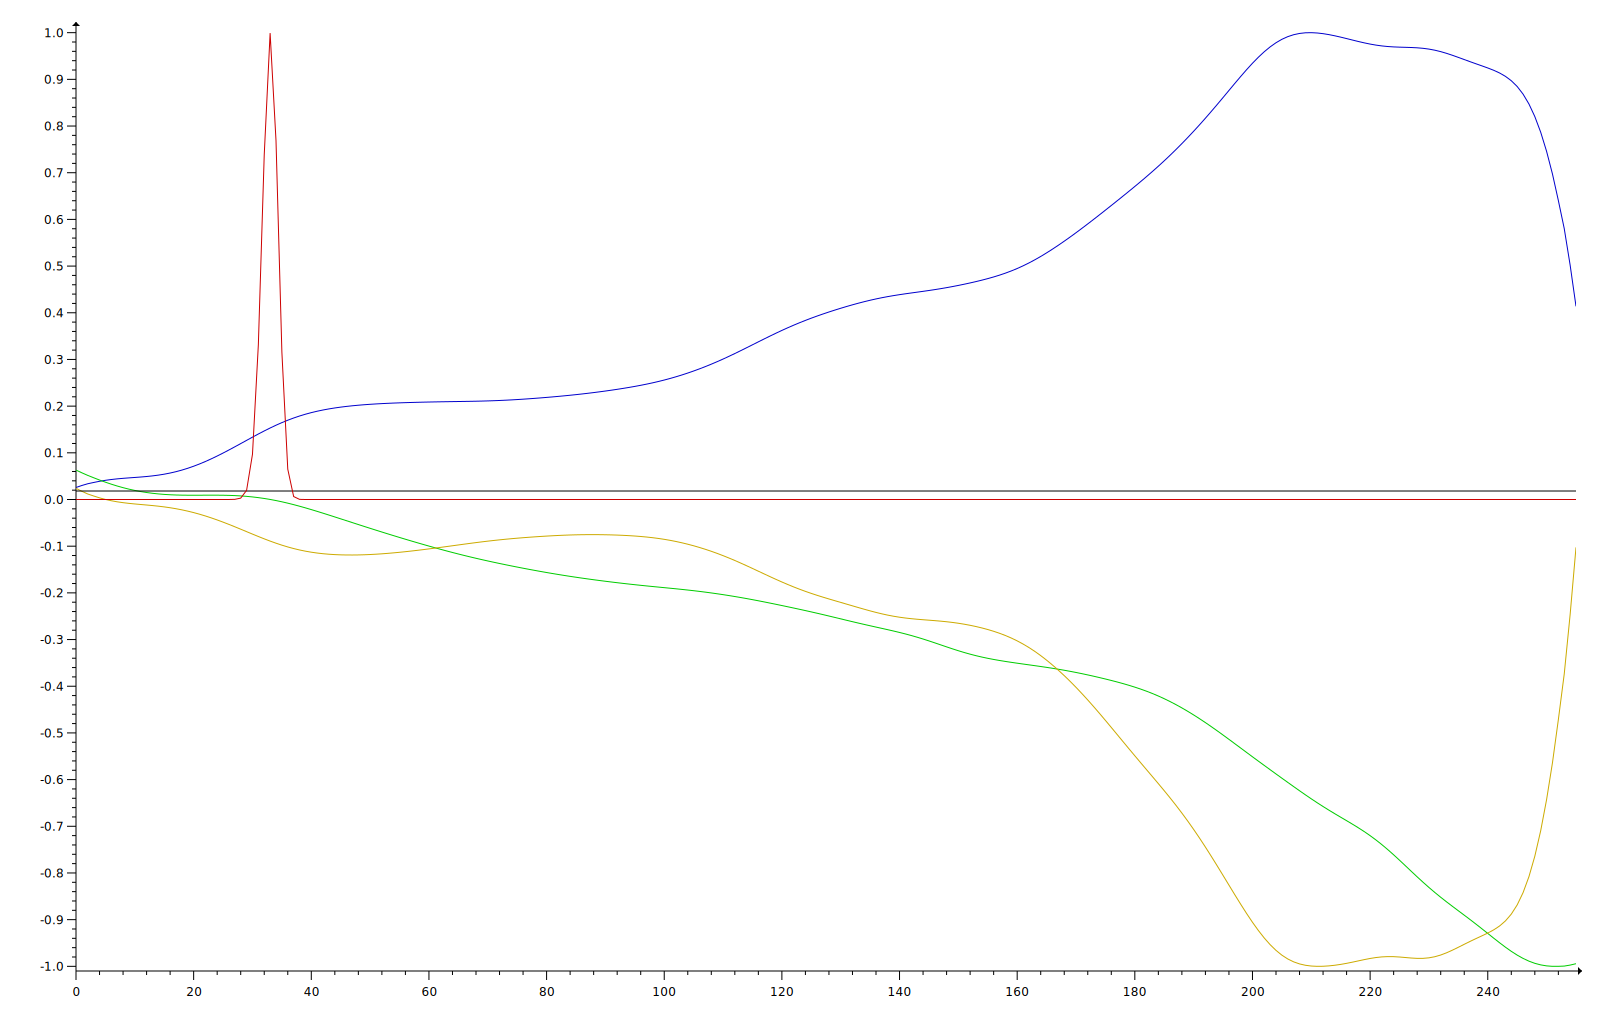
\includegraphics[width=0.35\textwidth]{images/r_g_skull}
		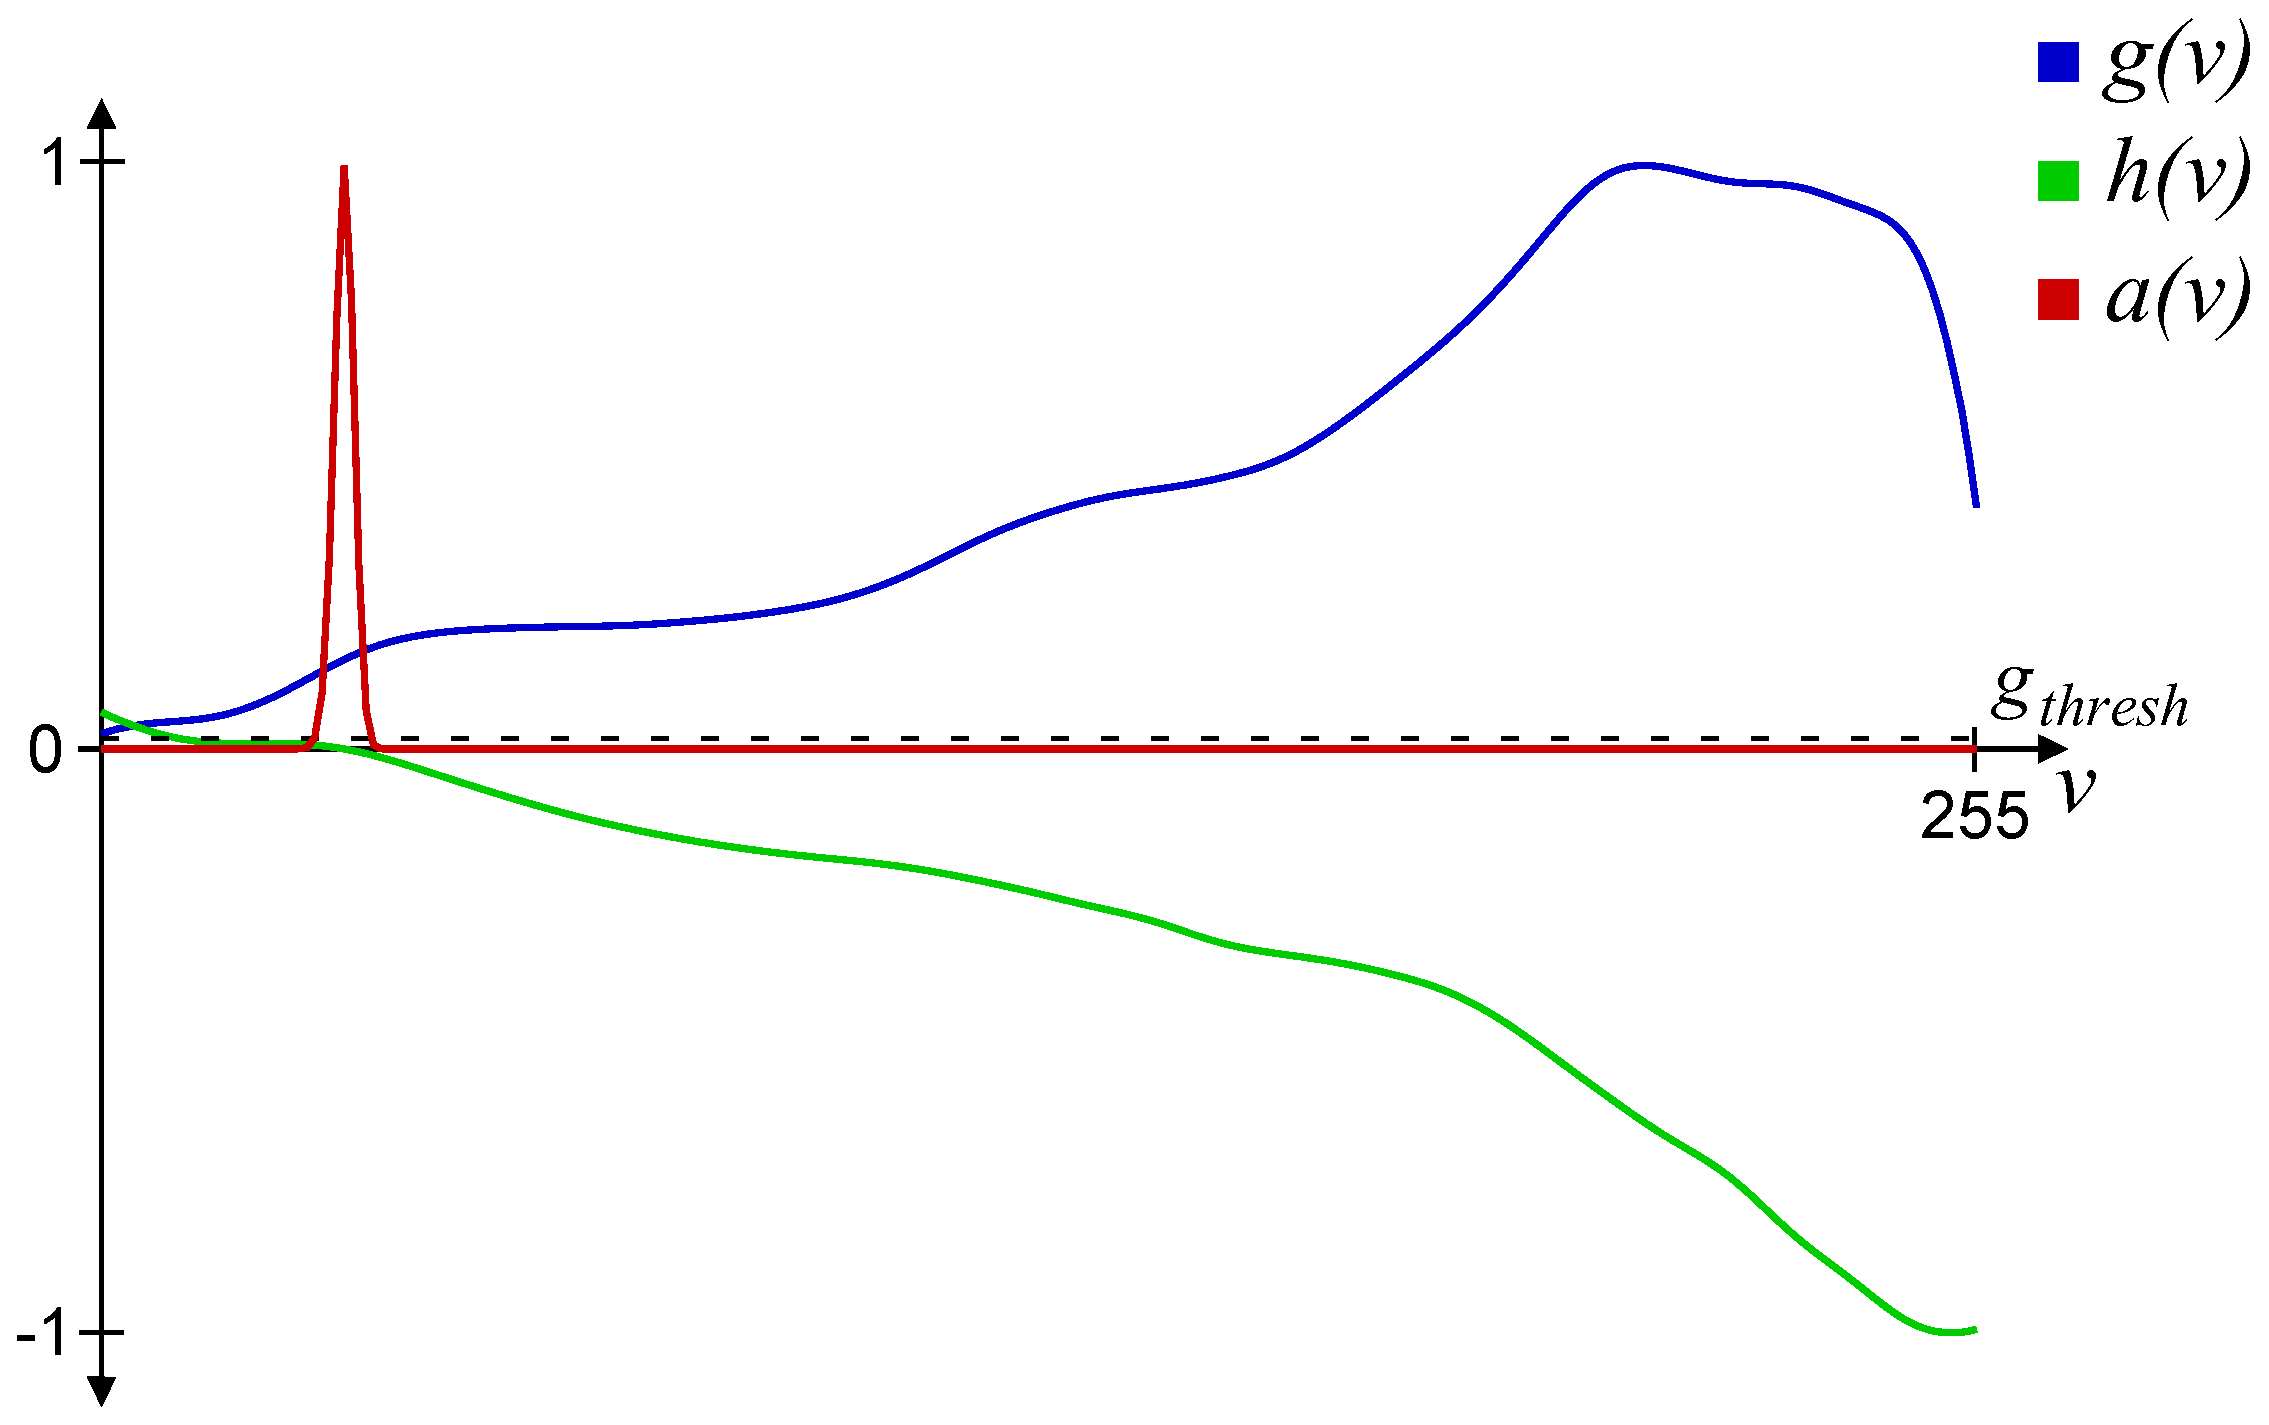
\includegraphics[width=0.65\textwidth]{images/r_g_skull_ft}
		\label{fig:r_skull_kd}
	}
	\subfigure[Método proposto.]
	{
		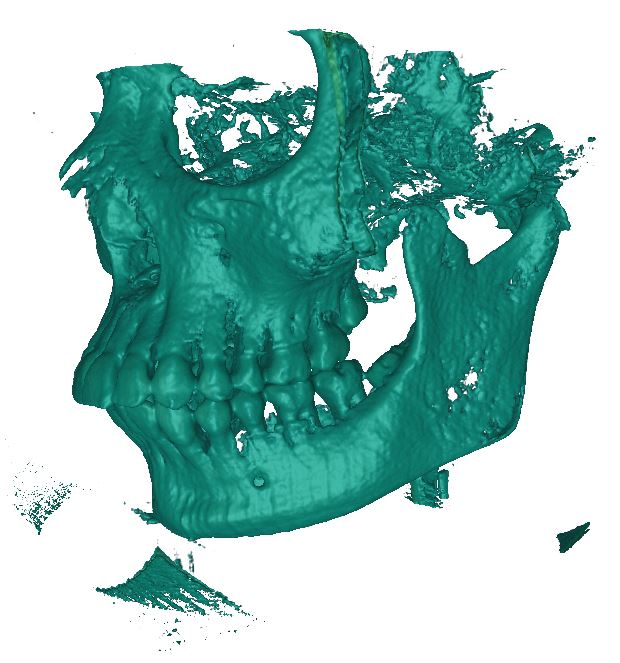
\includegraphics[width=0.35\textwidth]{images/r_m_skull}
		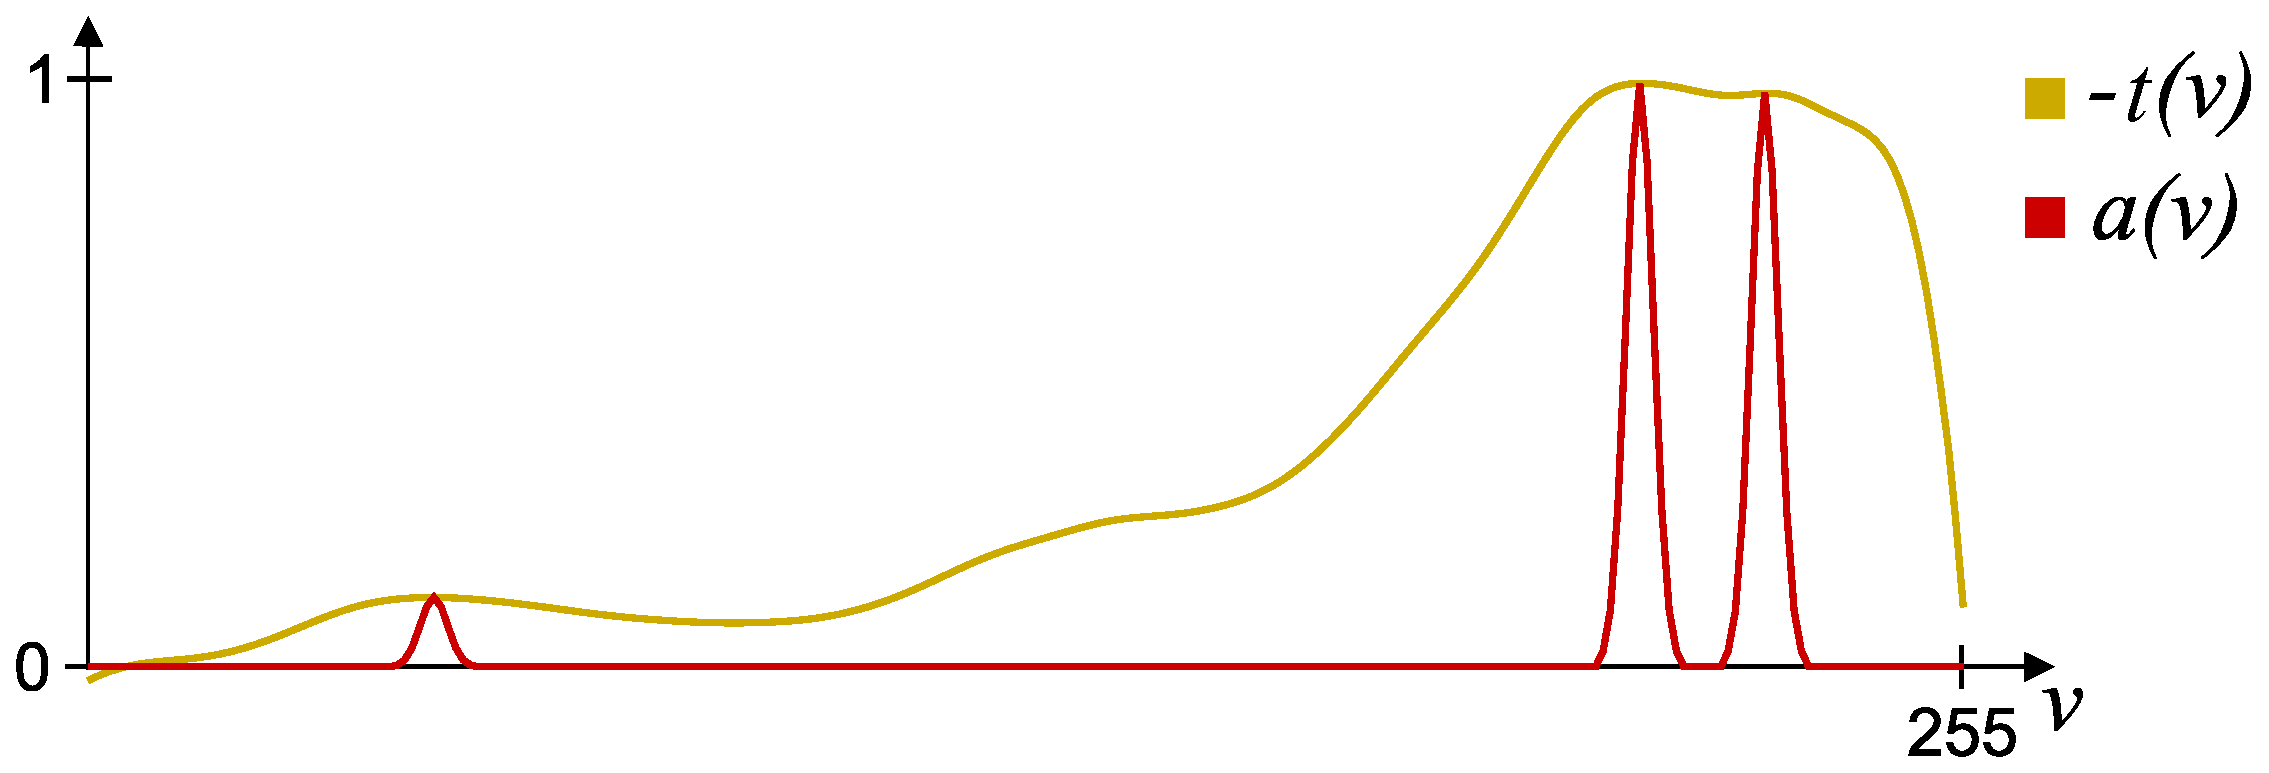
\includegraphics[width=0.65\textwidth]{images/r_m_skull_ft}	\label{fig:r_skull_mine}
	}
	\caption{Visualização e função de transferência do volume \quote{Skull}.}
	\label{fig:r_skull}
\end{figure}

%%%%%%%%%%%%%%%%%%%%%%%%%%%%%%%%%% Tooth %%%%%%%%%%%%%%%%%%%%%%%%%%%%%%%%%%%%%

	O volume seguinte é um dente envolvido por um material que causa a forma cilíndrica revelada nas visualizações da Figura~\ref{fig:r_tooth}. Como pode ser observado, tanto as funções de transferência como suas respectivas visualizações são semelhantes em ambos os métodos. Percebe-se apenas um ligeiro deslocamento da última fronteira obtida pelo método de \textit{Kindlmann~e~Durkin}, em relação à fronteira detectada  pelo método aqui proposto.
	
	Mais uma vez, não é possível avaliar apenas pela fatia do volume, qual fronteira é a mais correta. No entanto, vale ressaltar que o resultado exibido na Figura~\ref{fig:r_tooth}~\ref{fig:r_tooth_kd}, foi obtido após se encontrar o valor apropriado para o $ g_{thresh} $. Já o resultado exibido na Figura~\ref{fig:r_tooth}~\ref{fig:r_tooth_mine} não exigiu manipulação alguma da função de transferência.
	
\begin{figure}[h]
	\centering
	\subfigure[Método de \textit{Kindlmann e Durkin}.]
	{
		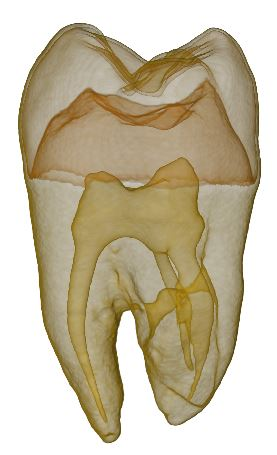
\includegraphics[width=0.35\textwidth]{images/r_g_tooth}
		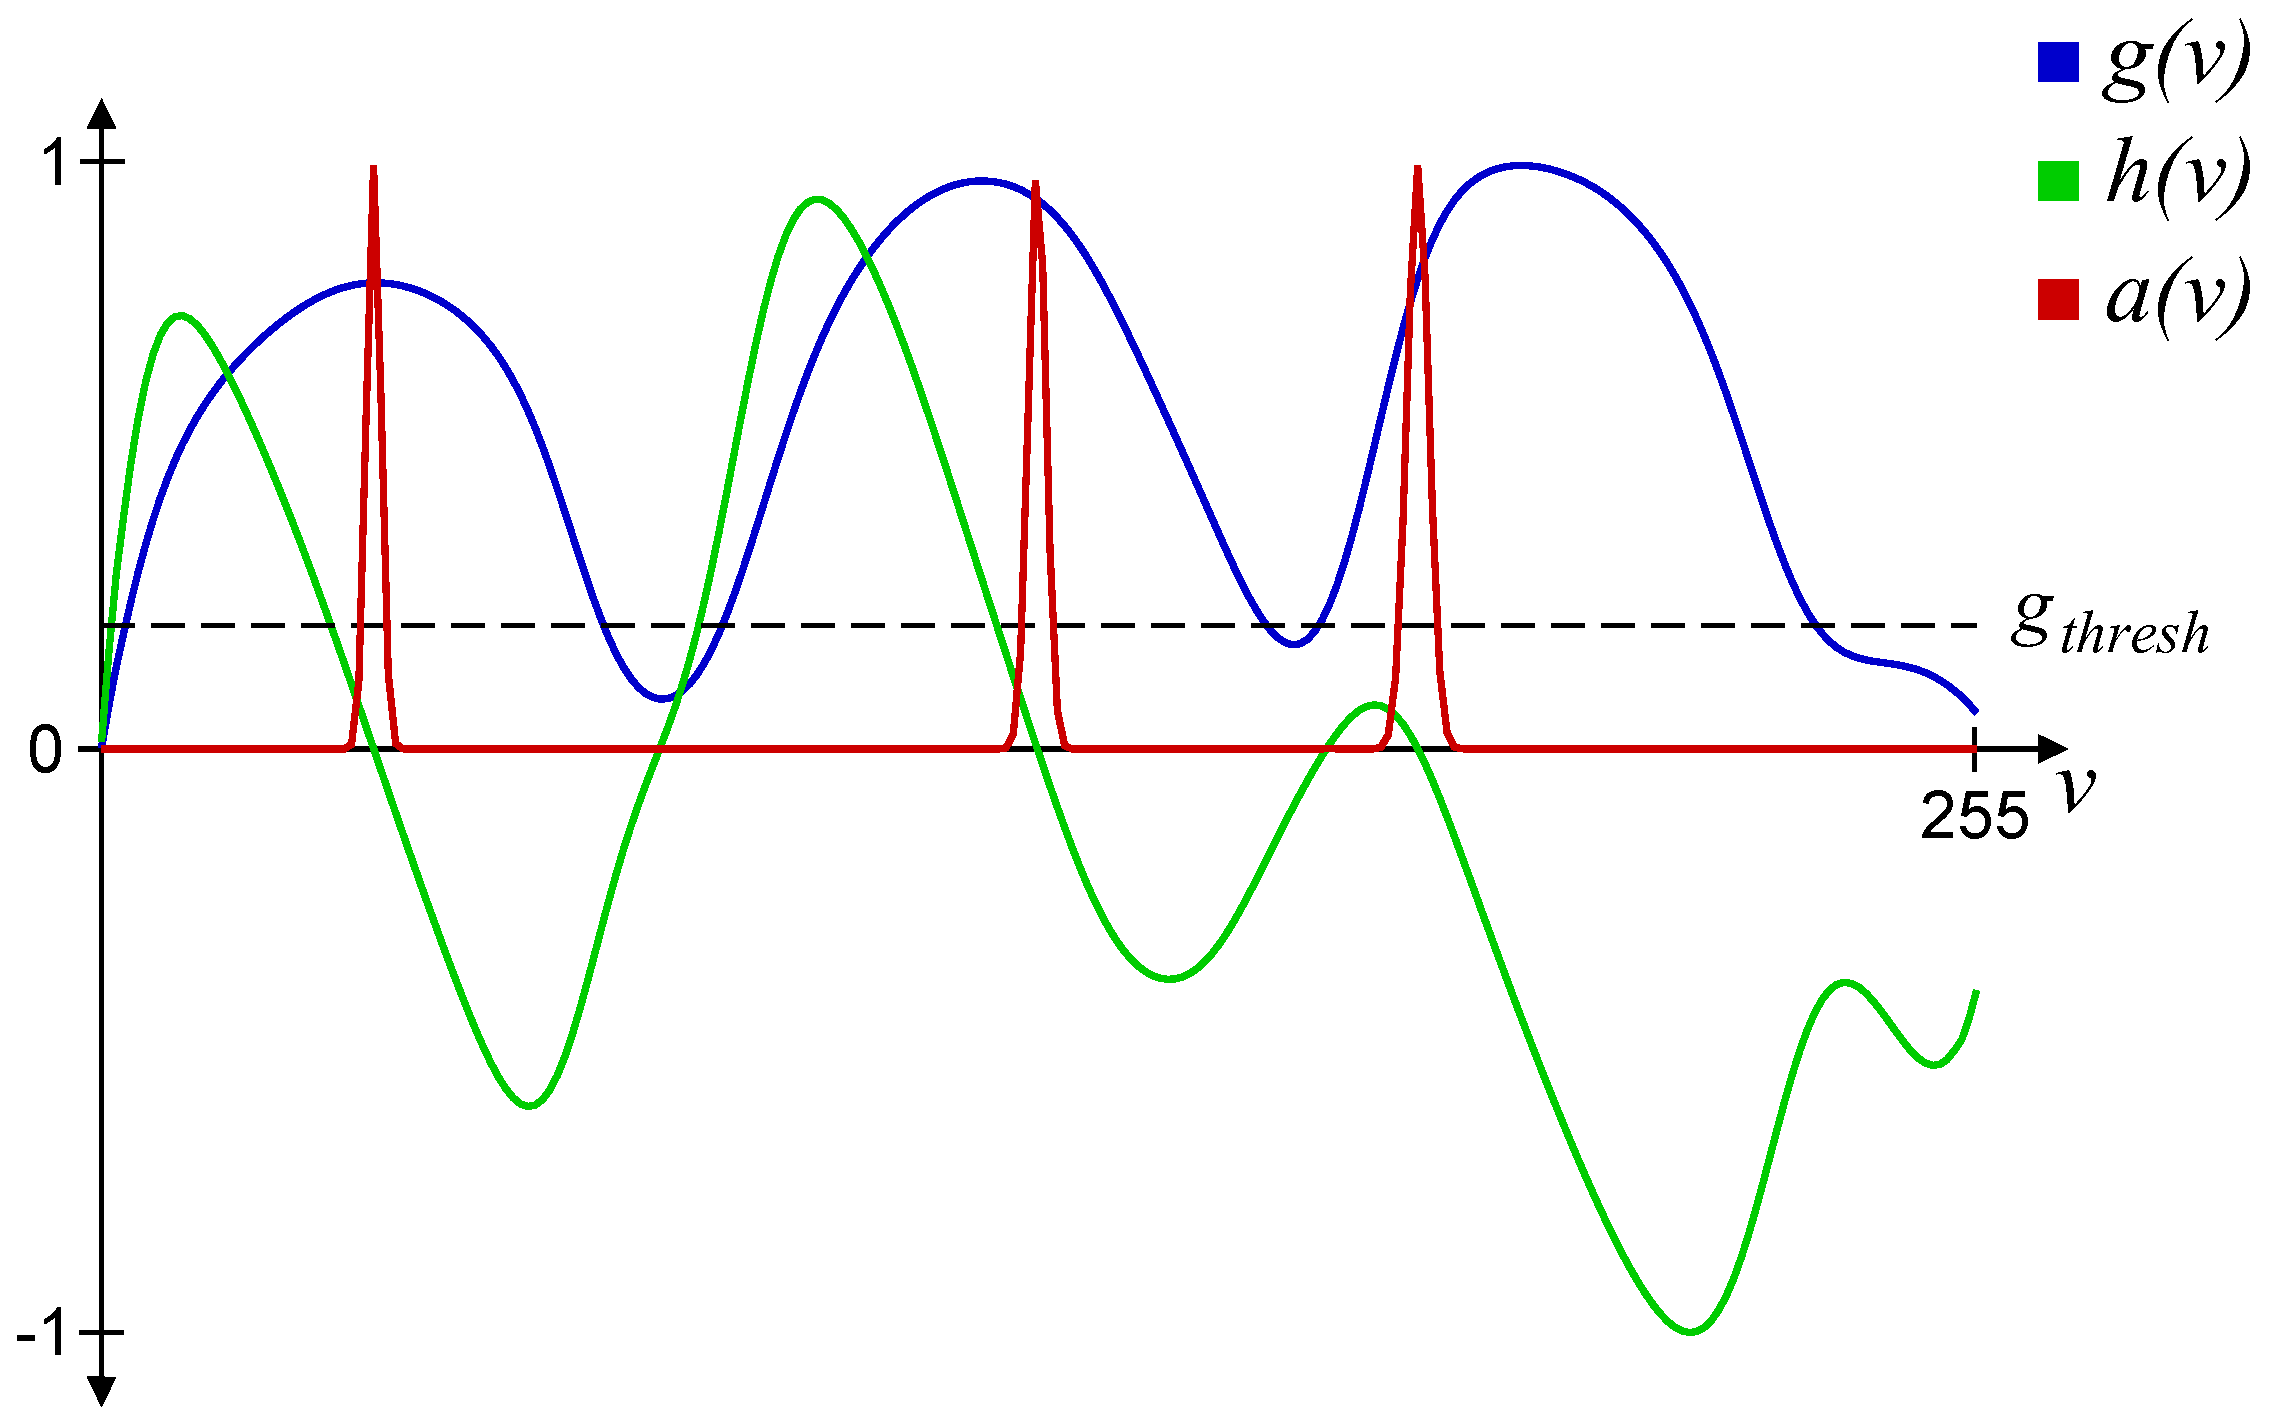
\includegraphics[width=0.65\textwidth]{images/r_g_tooth_ft}
		\label{fig:r_tooth_kd}
	}
	\subfigure[Método proposto.]
	{
		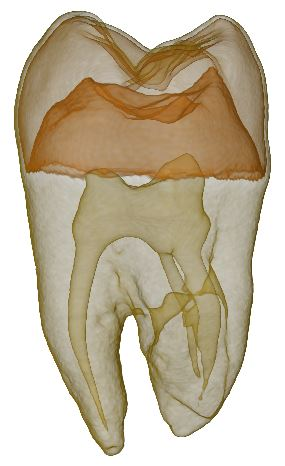
\includegraphics[width=0.35\textwidth]{images/r_m_tooth}
		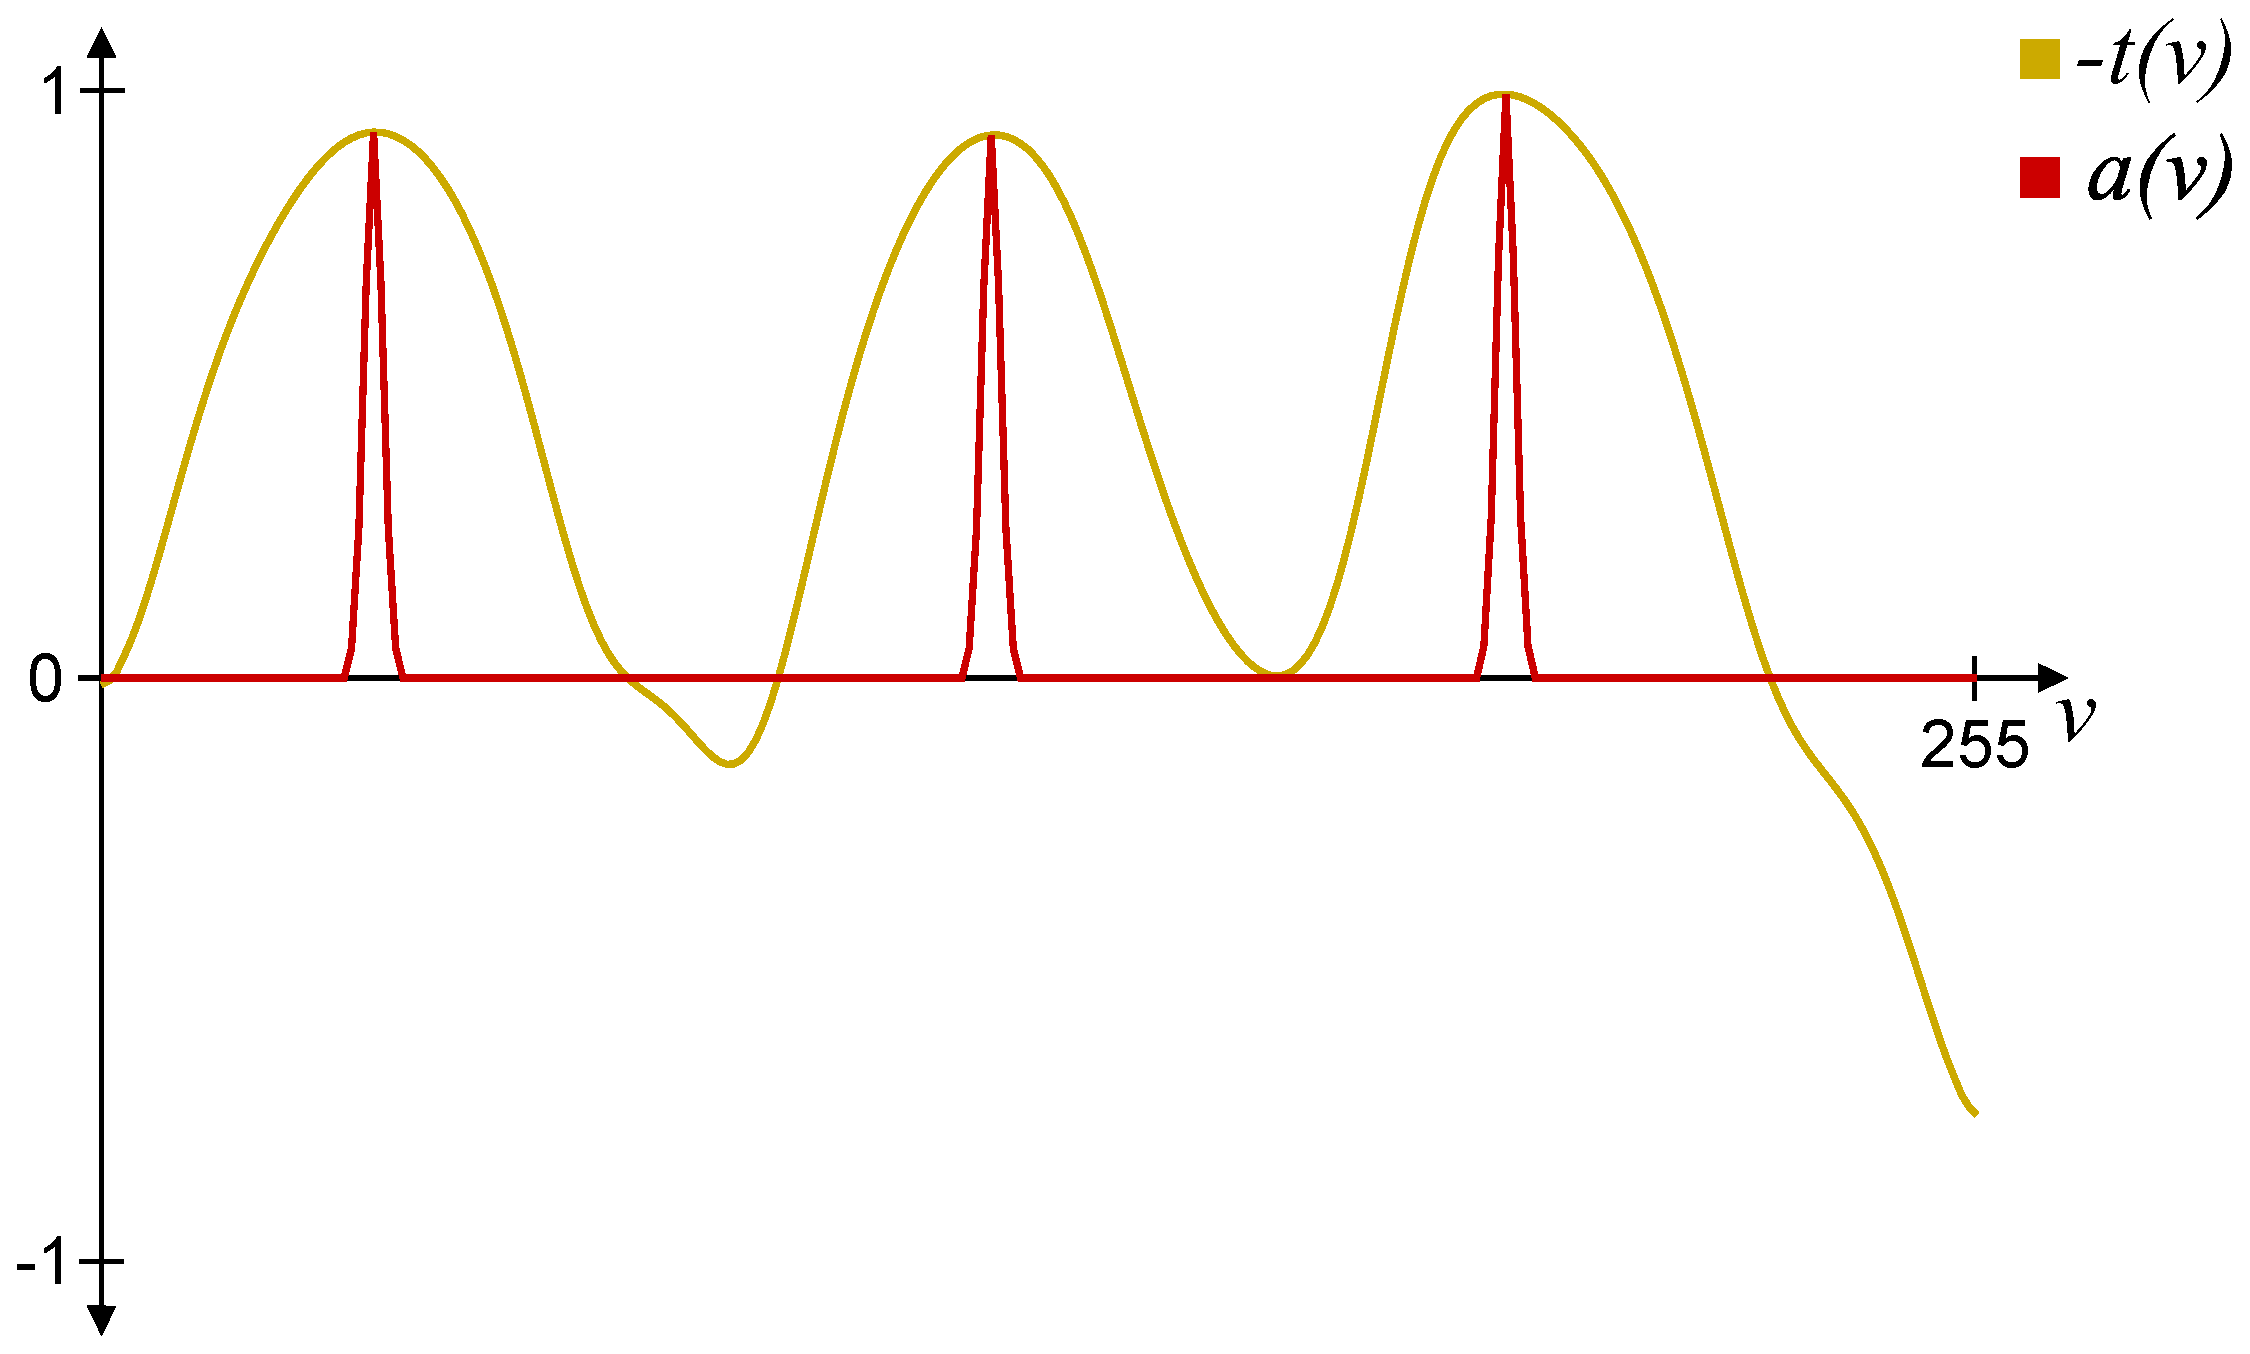
\includegraphics[width=0.65\textwidth]{images/r_m_tooth_ft}			\label{fig:r_tooth_mine}
	}
	\caption{Visualização e função de transferência de um dente.}
	\label{fig:r_tooth}
\end{figure}

	A Figura~\ref{fig:r_toothx_kd} mostra a visualização do dente, utilizando a FT gerada pelo método de \textit{Kindlmann e Durkin}, com $ g_{thresh} = 0 $ e com a metade do valor utilizado Na Figura~\ref{fig:r_tooth}~\ref{fig:r_tooth_kd}.

\begin{figure}[h]
	\centering
	\subfigure[Sem threshold.]
	{
		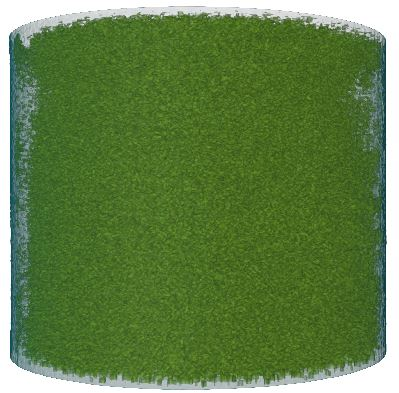
\includegraphics[width=0.35\textwidth]{images/r_g_tooth0}
		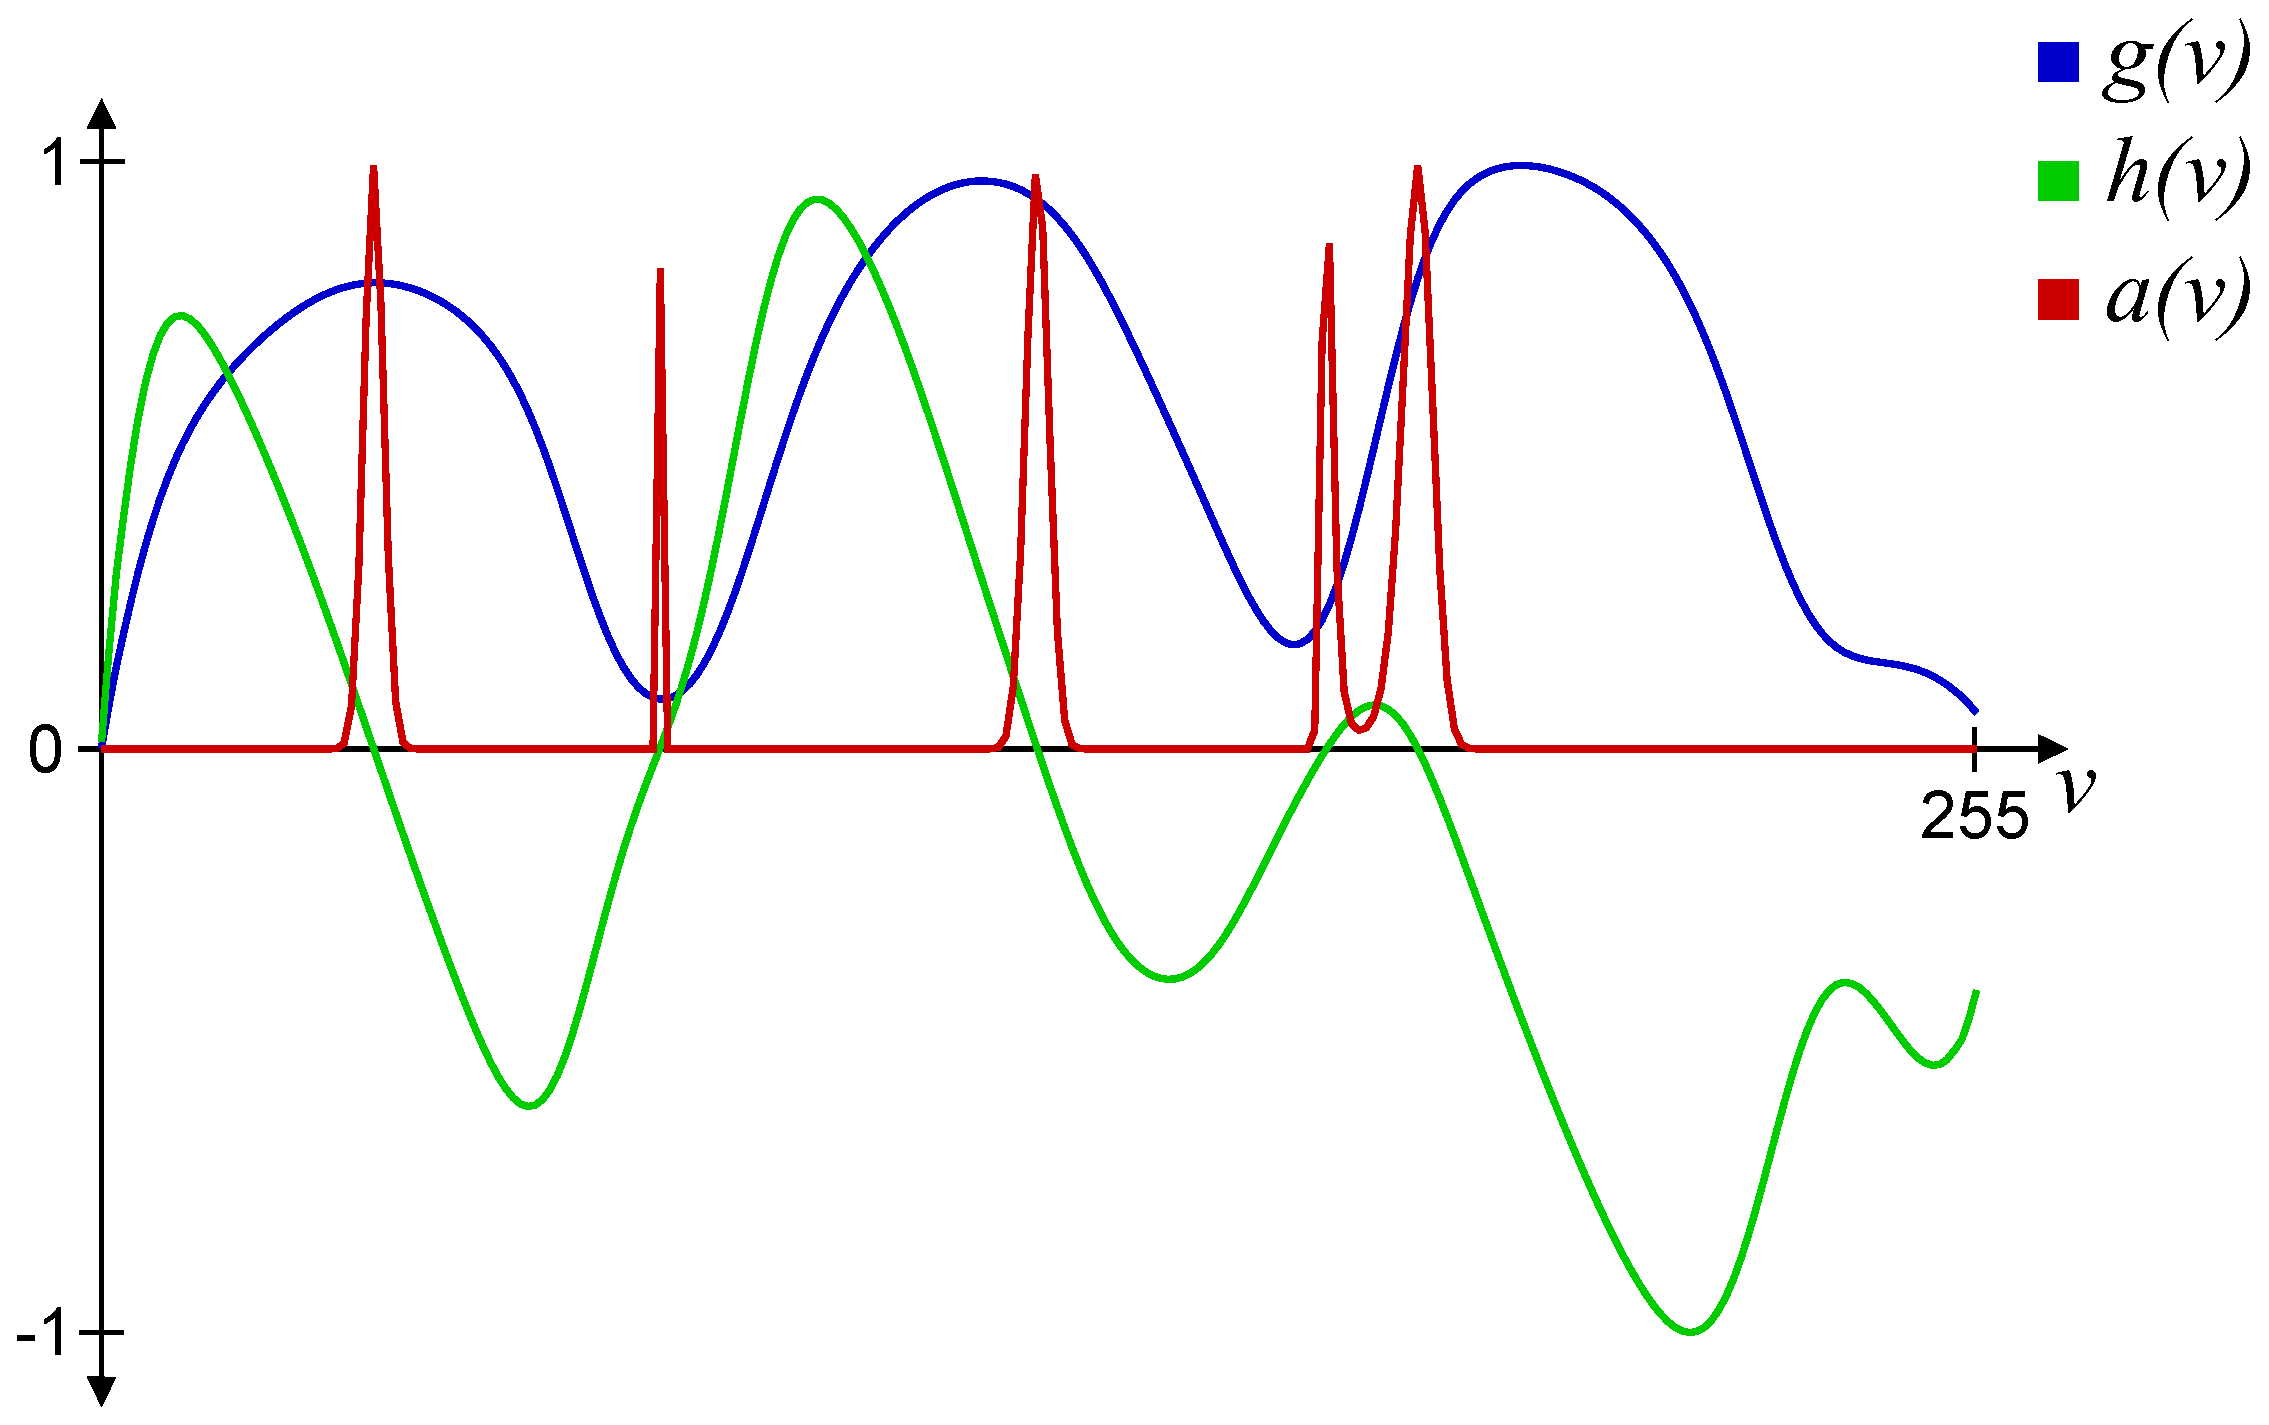
\includegraphics[width=0.65\textwidth]{images/r_g_tooth0_ft}
		\label{fig:r_tooth0_kd}
	}
	\subfigure[Com threshold menor que o apropriado.]
	{
		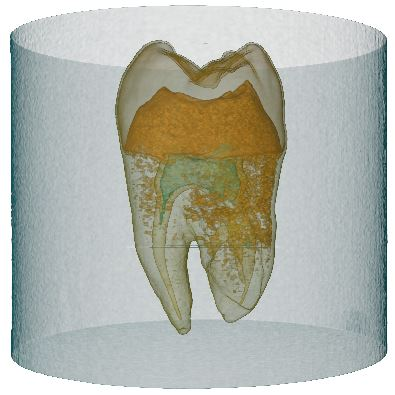
\includegraphics[width=0.35\textwidth]{images/r_g_tooth1}
		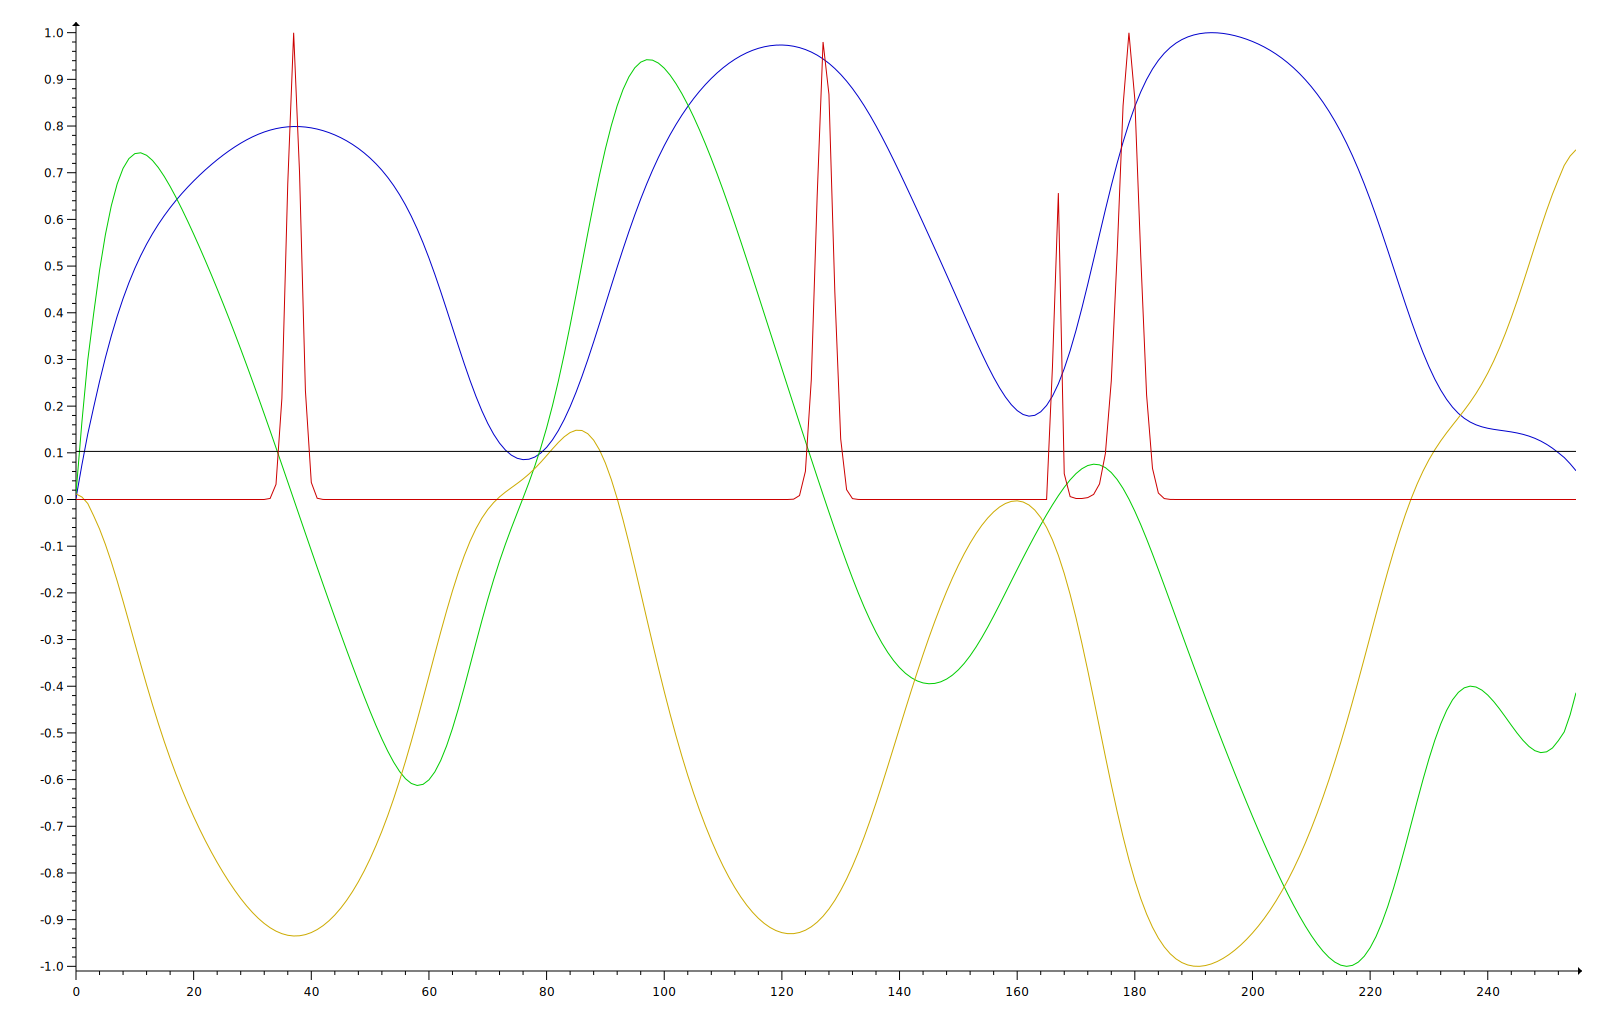
\includegraphics[width=0.65\textwidth]{images/r_g_tooth1_ft}\label{fig:r_tooth1_kd}
	}
	\caption{Visualização e função de transferência de um dente.}
	\label{fig:r_toothx_kd}
\end{figure}

%%%%%%%%%%%%%%%%%%%%%%%%%%%%%%%%%%% Bonsai %%%%%%%%%%%%%%%%%%%%%%%%%%%%%%%%%%%%%
%	O bonsai já é um volume conhecido na literatura, principalmente pelo ruído presente acima das raízes, que possui valor muito próximo ao das folhas. Portanto, para visualizá-lo corretamente, é preciso remover as isosuperfícies que correspondem a esse ruído e aumentar a largura da função de transferência até que até que as folhas apareçam novamente. No método 1D de \textit{Kindlmann~e~Durkin} esse processo é feito através do $ g_{thresh} $, enquanto no método desta dissertação desliga-se as isosuperfícies através da interface, como já explicado na Seção~\ref{sec:my.tf}.
%	
%	Como pode ser observado na Figura~\ref{fig:r_m_bonsai}, as funções de transferência são bem distintas, apesar de resultarem em visualizações quase idênticas. Então, cabe observar que, dentro da proposta de realçar como fronteira a isosuperfície que possui maior derivada, o método proposto por esta dissertação apresenta uma função de transferência mais adequada.
%	
%\begin{figure}[h]
%	\centering
%	\subfigure[Método de \textit{Kindlmann e Durkin}.]
%	{
%		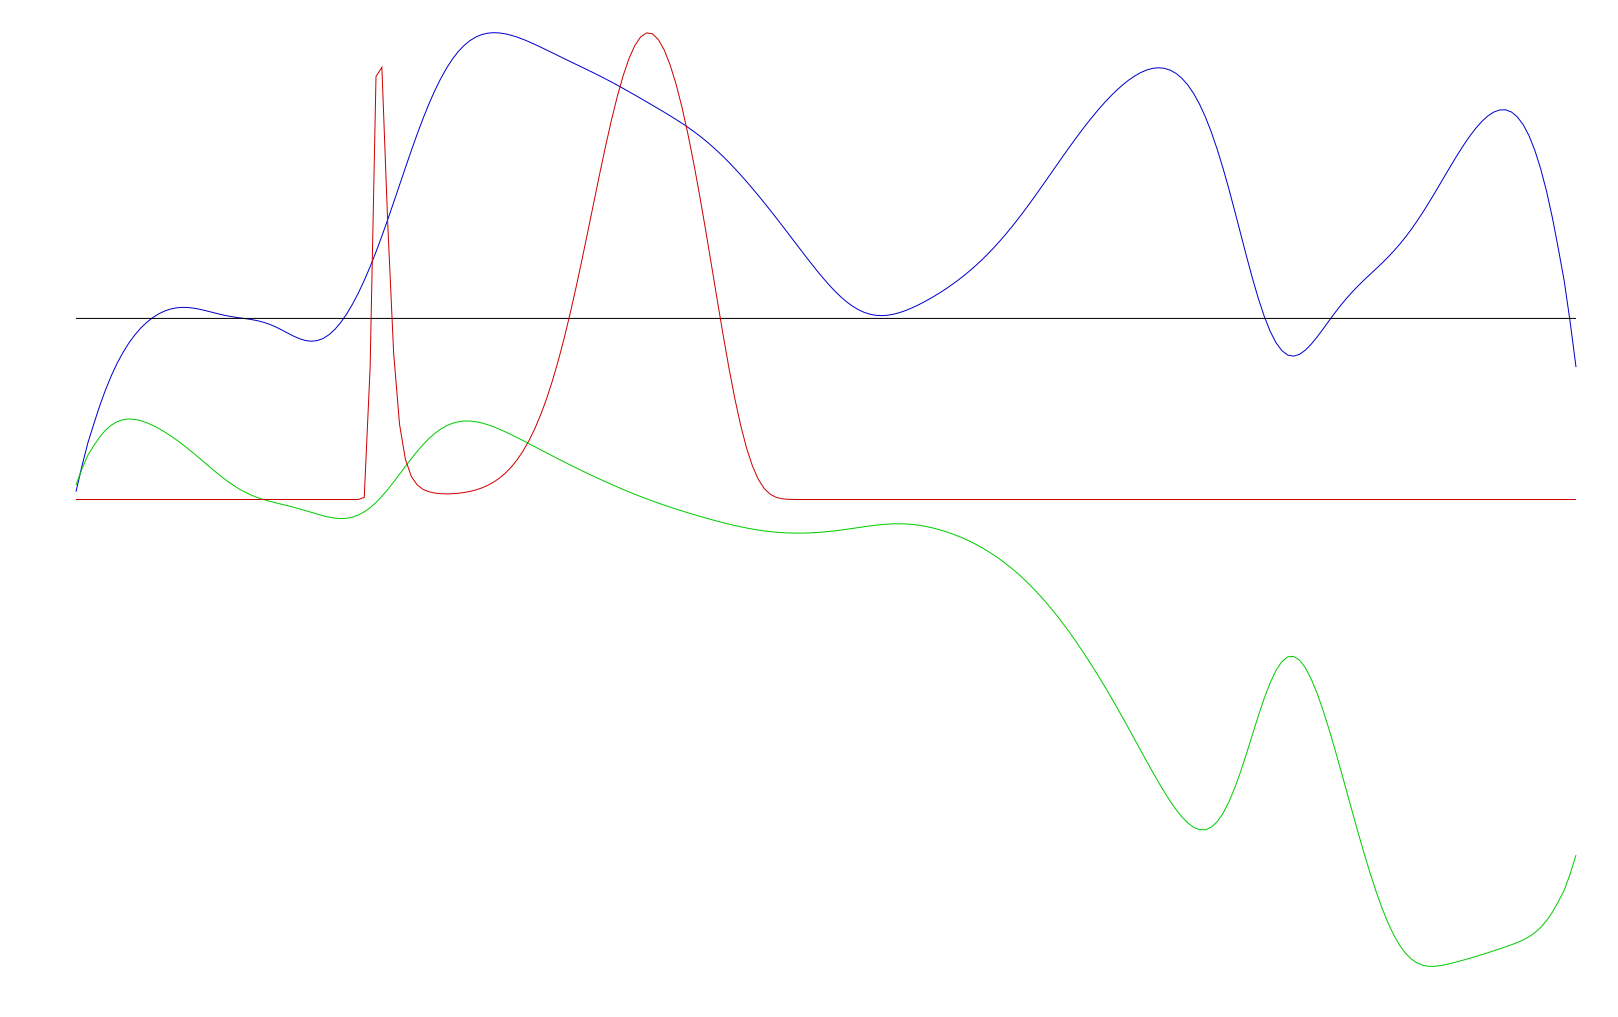
\includegraphics[width=0.7\textwidth]{images/r_g_bonsai_ft}
%		\label{fig:r_bonsai_kd_ft}
%	}
%	\subfigure[Método proposto.]
%	{
%		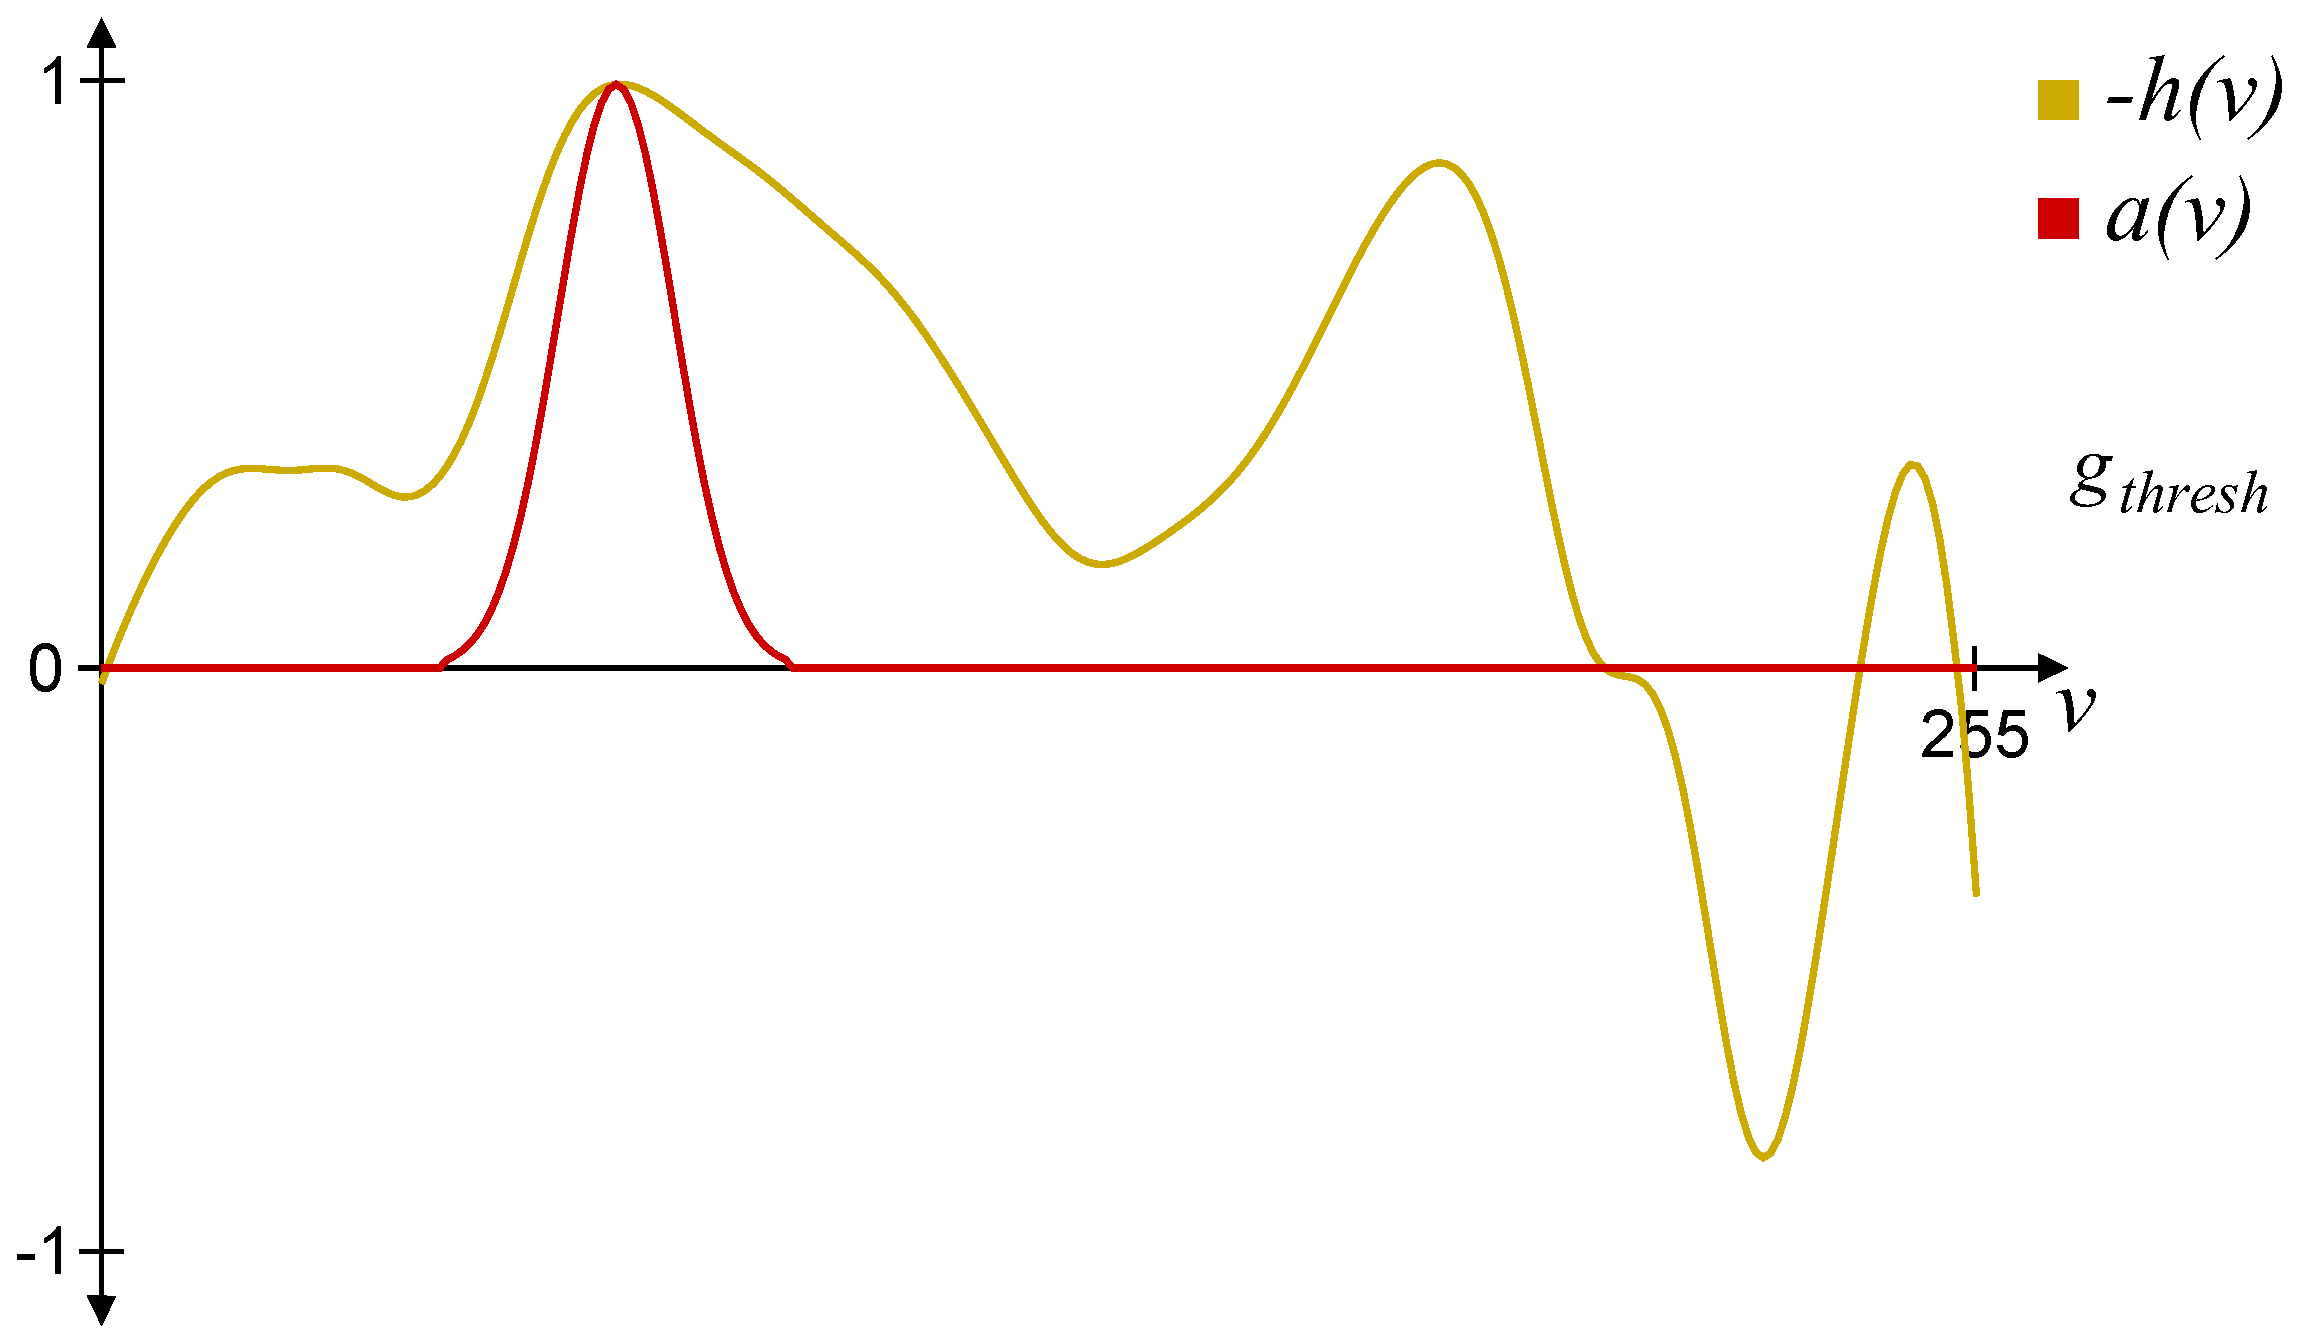
\includegraphics[width=0.7\textwidth]{images/r_m_bonsai_ft}			\label{fig:r_bonsai_mine_ft}
%	}
%	\subfigure[Método de \textit{Kindlmann e Durkin}.]
%	{
%		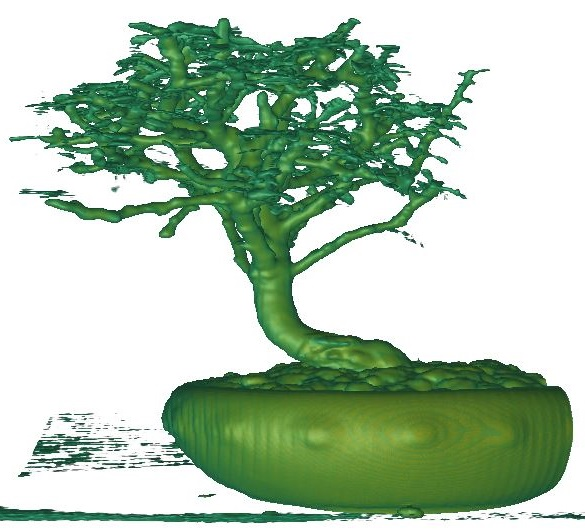
\includegraphics[width=0.47\textwidth]{images/r_g_bonsai}
%		\label{fig:r_bonsai_kd}
%	}
%	\subfigure[Método proposto.]
%	{
%		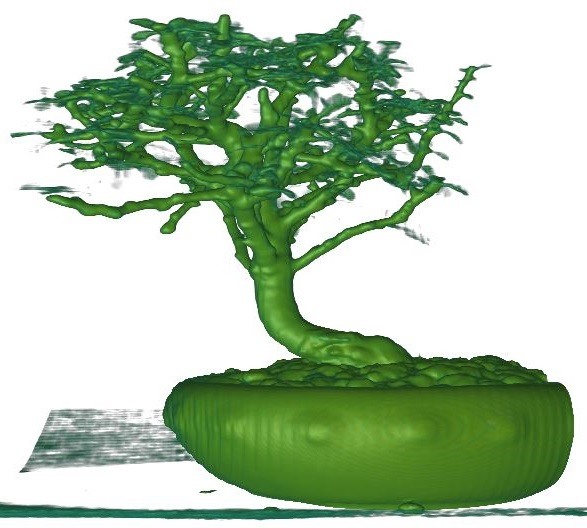
\includegraphics[width=0.47\textwidth]{images/r_m_bonsai}
%		\label{fig:r_bonsai_mine}
%	}
%	\caption{Visualização e função de transferência do bonsai.}
%	\label{fig:r_m_bonsai}
%\end{figure}

%%%%%%%%%%%%%%%%%%%%%%%%%%%%%%%%%% X %%%%%%%%%%%%%%%%%%%%%%%%%%%%%%%%%%%%%
\newpage
	Os dois volumes seguintes não apresentaram discrepância entre os métodos. Então, os resultados obtidos serão ilustrados e comentados, mas não comparados com o método de \textit{Kindlmann~e~Durkin}.
\clearpage
	A Figura~\ref{fig:r_m_carp} mostra a função de transferência obtida com o método desta dissertação, bem como a visualização volumétrica resultante. As duas primeiras fronteiras vistas na FT correspondem respectivamente ao exterior e ao exoesqueleto da carpa. As outras duas representam regiões pequenas do exoesqueleto de maior intensidade. A Figura~\ref{fig:r_m_carp}~\ref{fig:r_m_carp_exo} mostra apenas o exoesqueleto da carpa. Para isso, a fronteira referente ao exterior da carpa foi desligada e a opacidade máxima da função de transferência aumentada.
	
\begin{figure}[h]
	\centering
	\subfigure[]
	{
		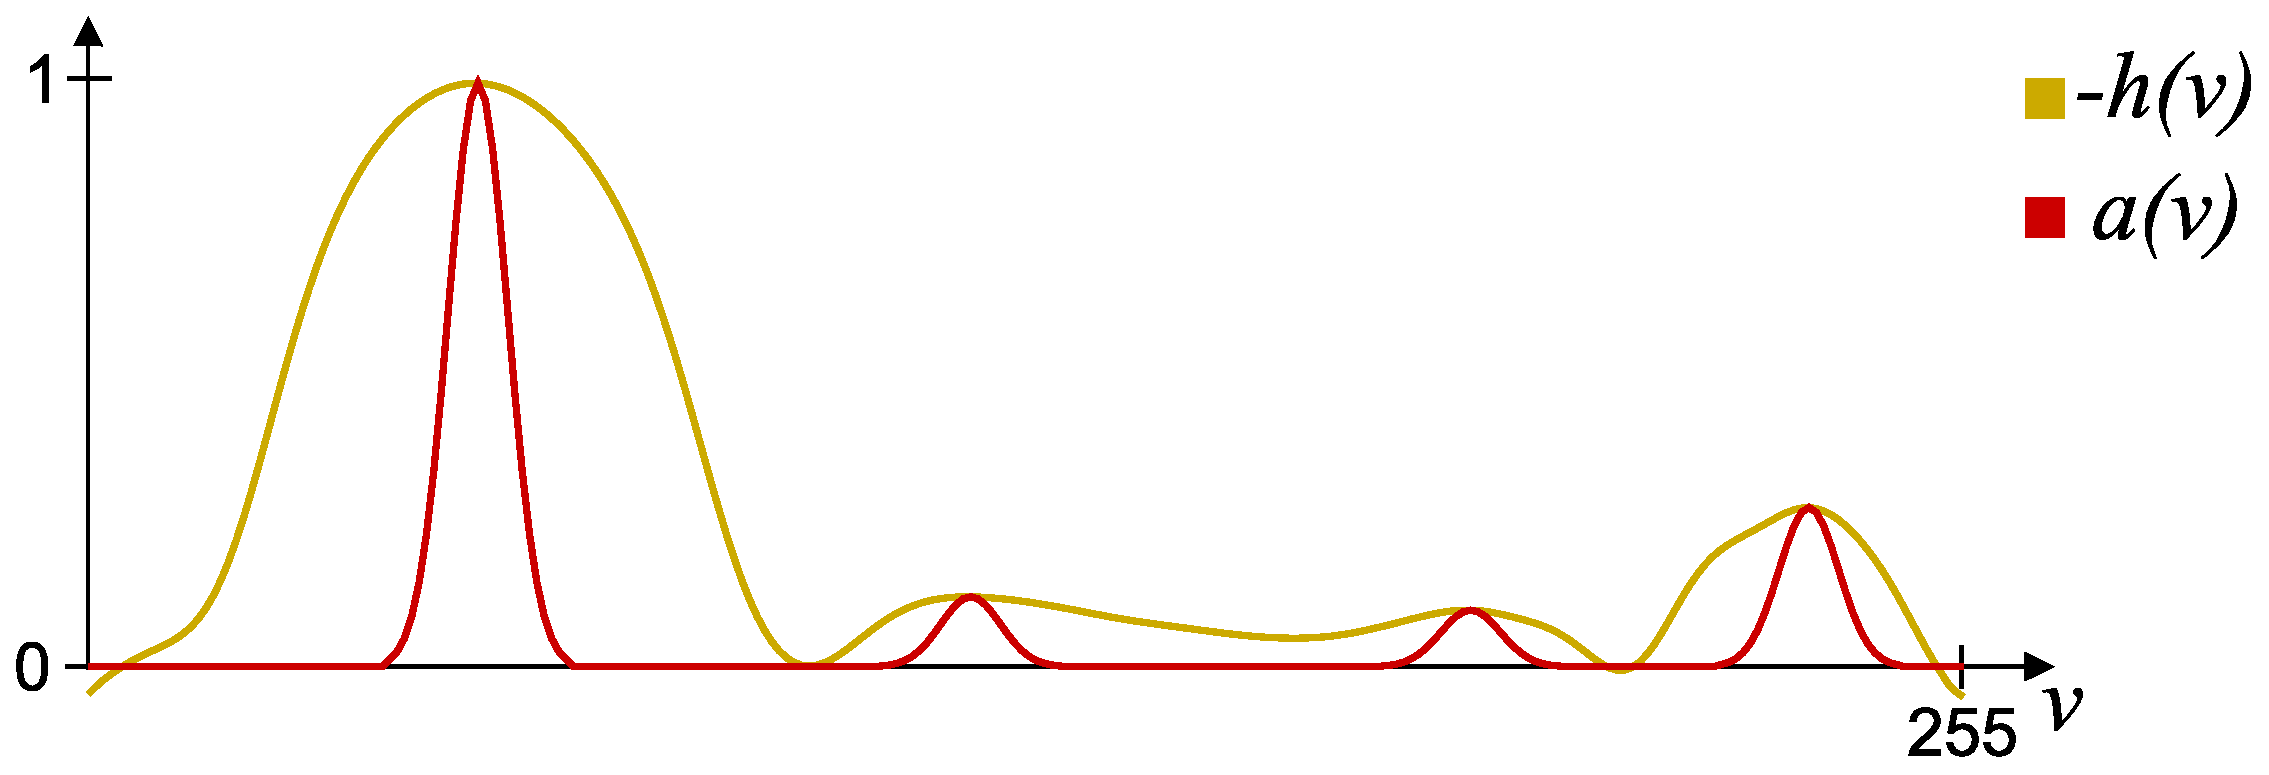
\includegraphics[width=0.7\textwidth]{images/r_m_carp_ft}
		\label{fig:r_m_carp_ft}
	}
	\subfigure[]
	{
		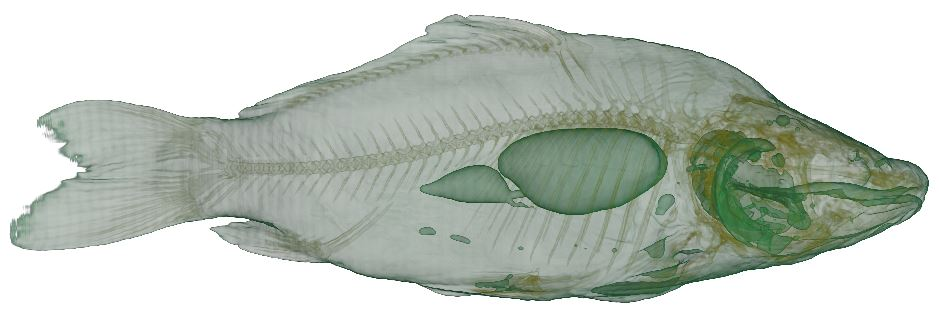
\includegraphics[width=0.8\textwidth]{images/r_m_carp}
		\label{fig:r_m_carp_side}
	}
	\subfigure[]
	{
		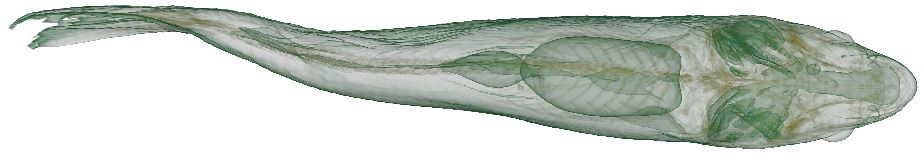
\includegraphics[width=0.8\textwidth]{images/r_m_carp_up}
		\label{fig:r_m_carp_up}
	}
	\subfigure[]
	{
		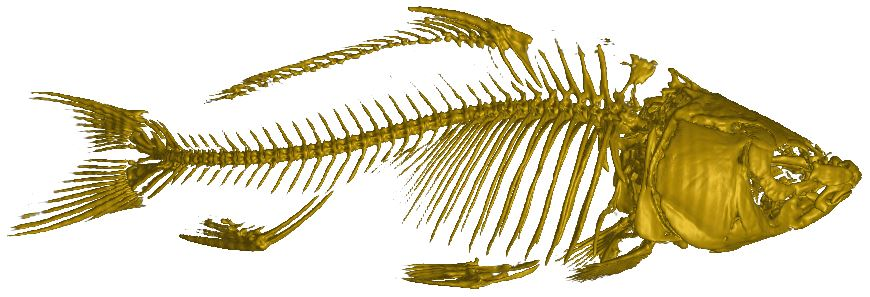
\includegraphics[width=0.8\textwidth]{images/r_m_carp_exo}
		\label{fig:r_m_carp_exo}
	}
	\caption{Carpa.}
	\label{fig:r_m_carp}
\end{figure}

%\begin{figure}[h]
%	\centering
%	\subfigure[]
%	{
%		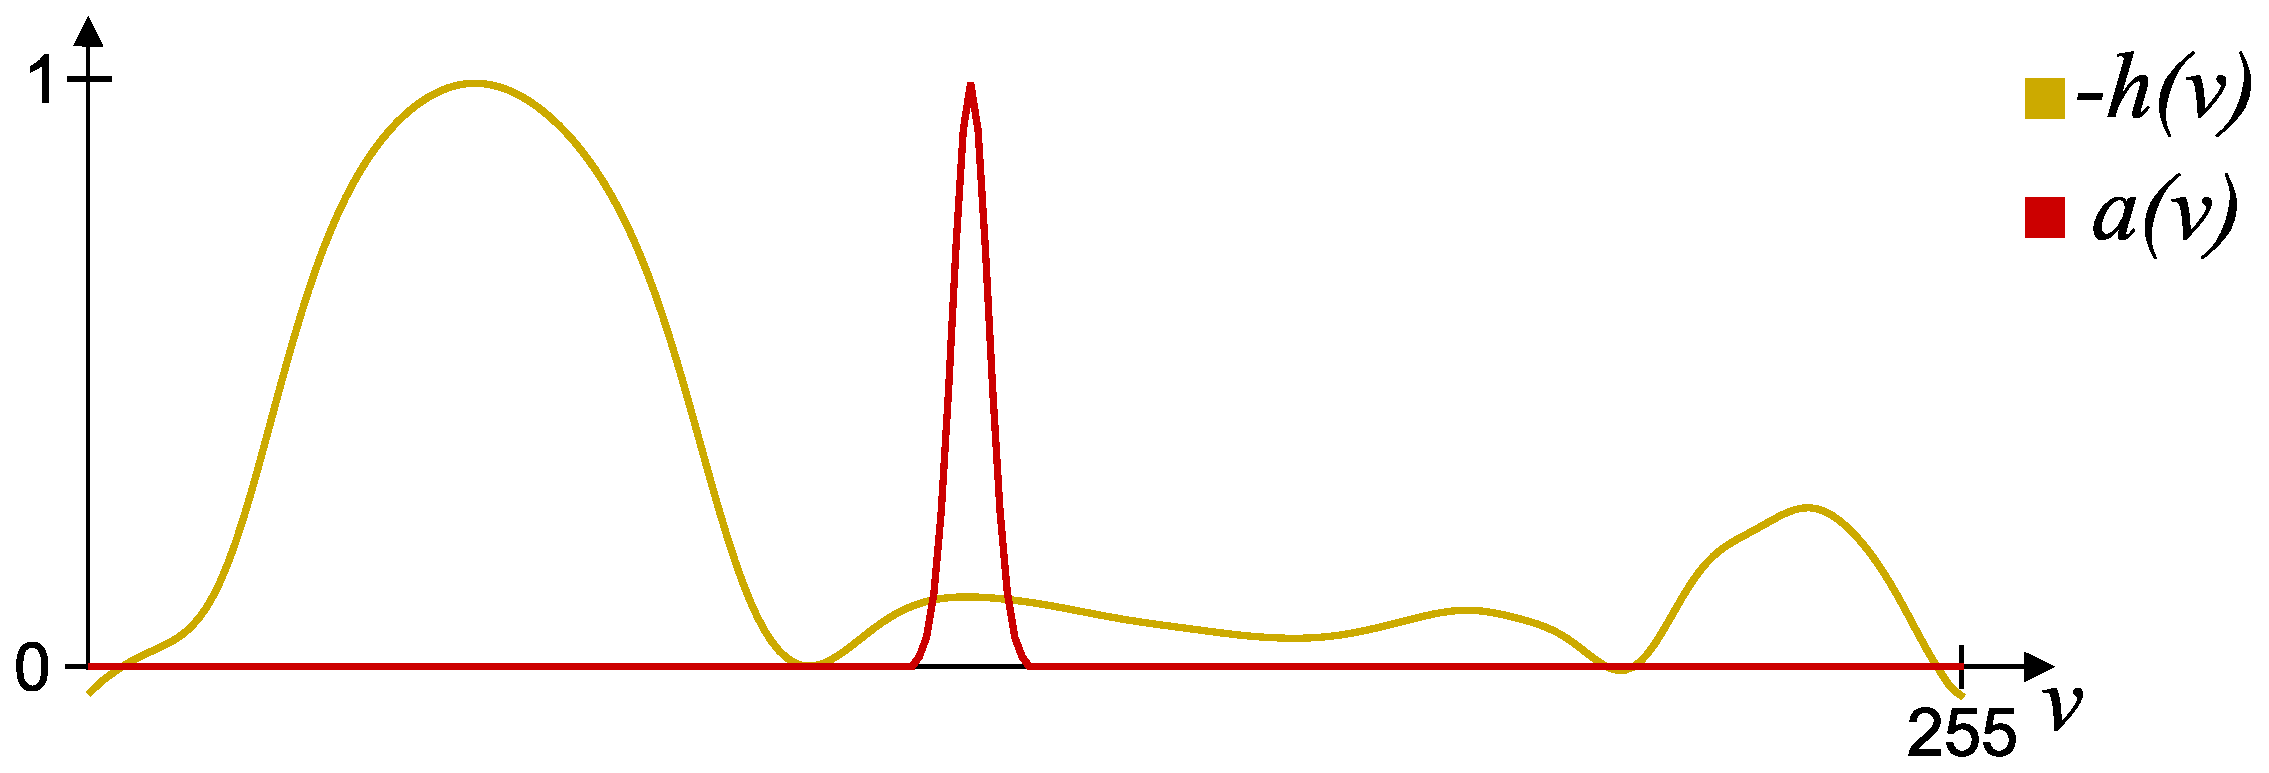
\includegraphics[width=0.7\textwidth]{images/r_m_carp_exo_ft}
%	}
%	\subfigure[]
%	{
%		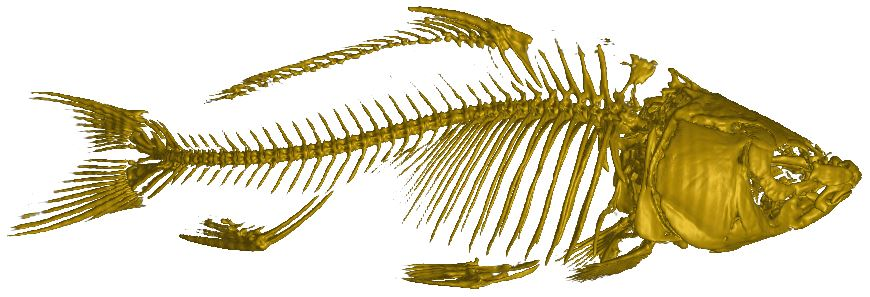
\includegraphics[width=0.8\textwidth]{images/r_m_carp_exo}
%	}	
%	\caption{Exoesqueleto da carpa.}
%	\label{fig:r_m_carp_exo}
%\end{figure}
\newpage
	O volume \quote{Knee} apresenta uma peculiaridade. Ele contém duas fronteiras: a externa, que aparenta ser a pele, e a interna, que é estrutura óssea do joelho. A fronteira interna abrange um grande intervalo de valores. Então, para poder visualizá-la separadamente, foi preciso desligar a fronteira externa e aumentar consideravelmente a largura da função de transferência. Essa tarefa seria mais complicada em um método onde as fronteiras não são associadas a isovalores, pois ao aumentar muito a largura da função de transferência, as fronteiras se uniriam. Isso tornaria mais difícil sua separação, para visualizar apenas a estrutura óssea.

\begin{figure}[h]
	\centering
	\subfigure[]
	{
		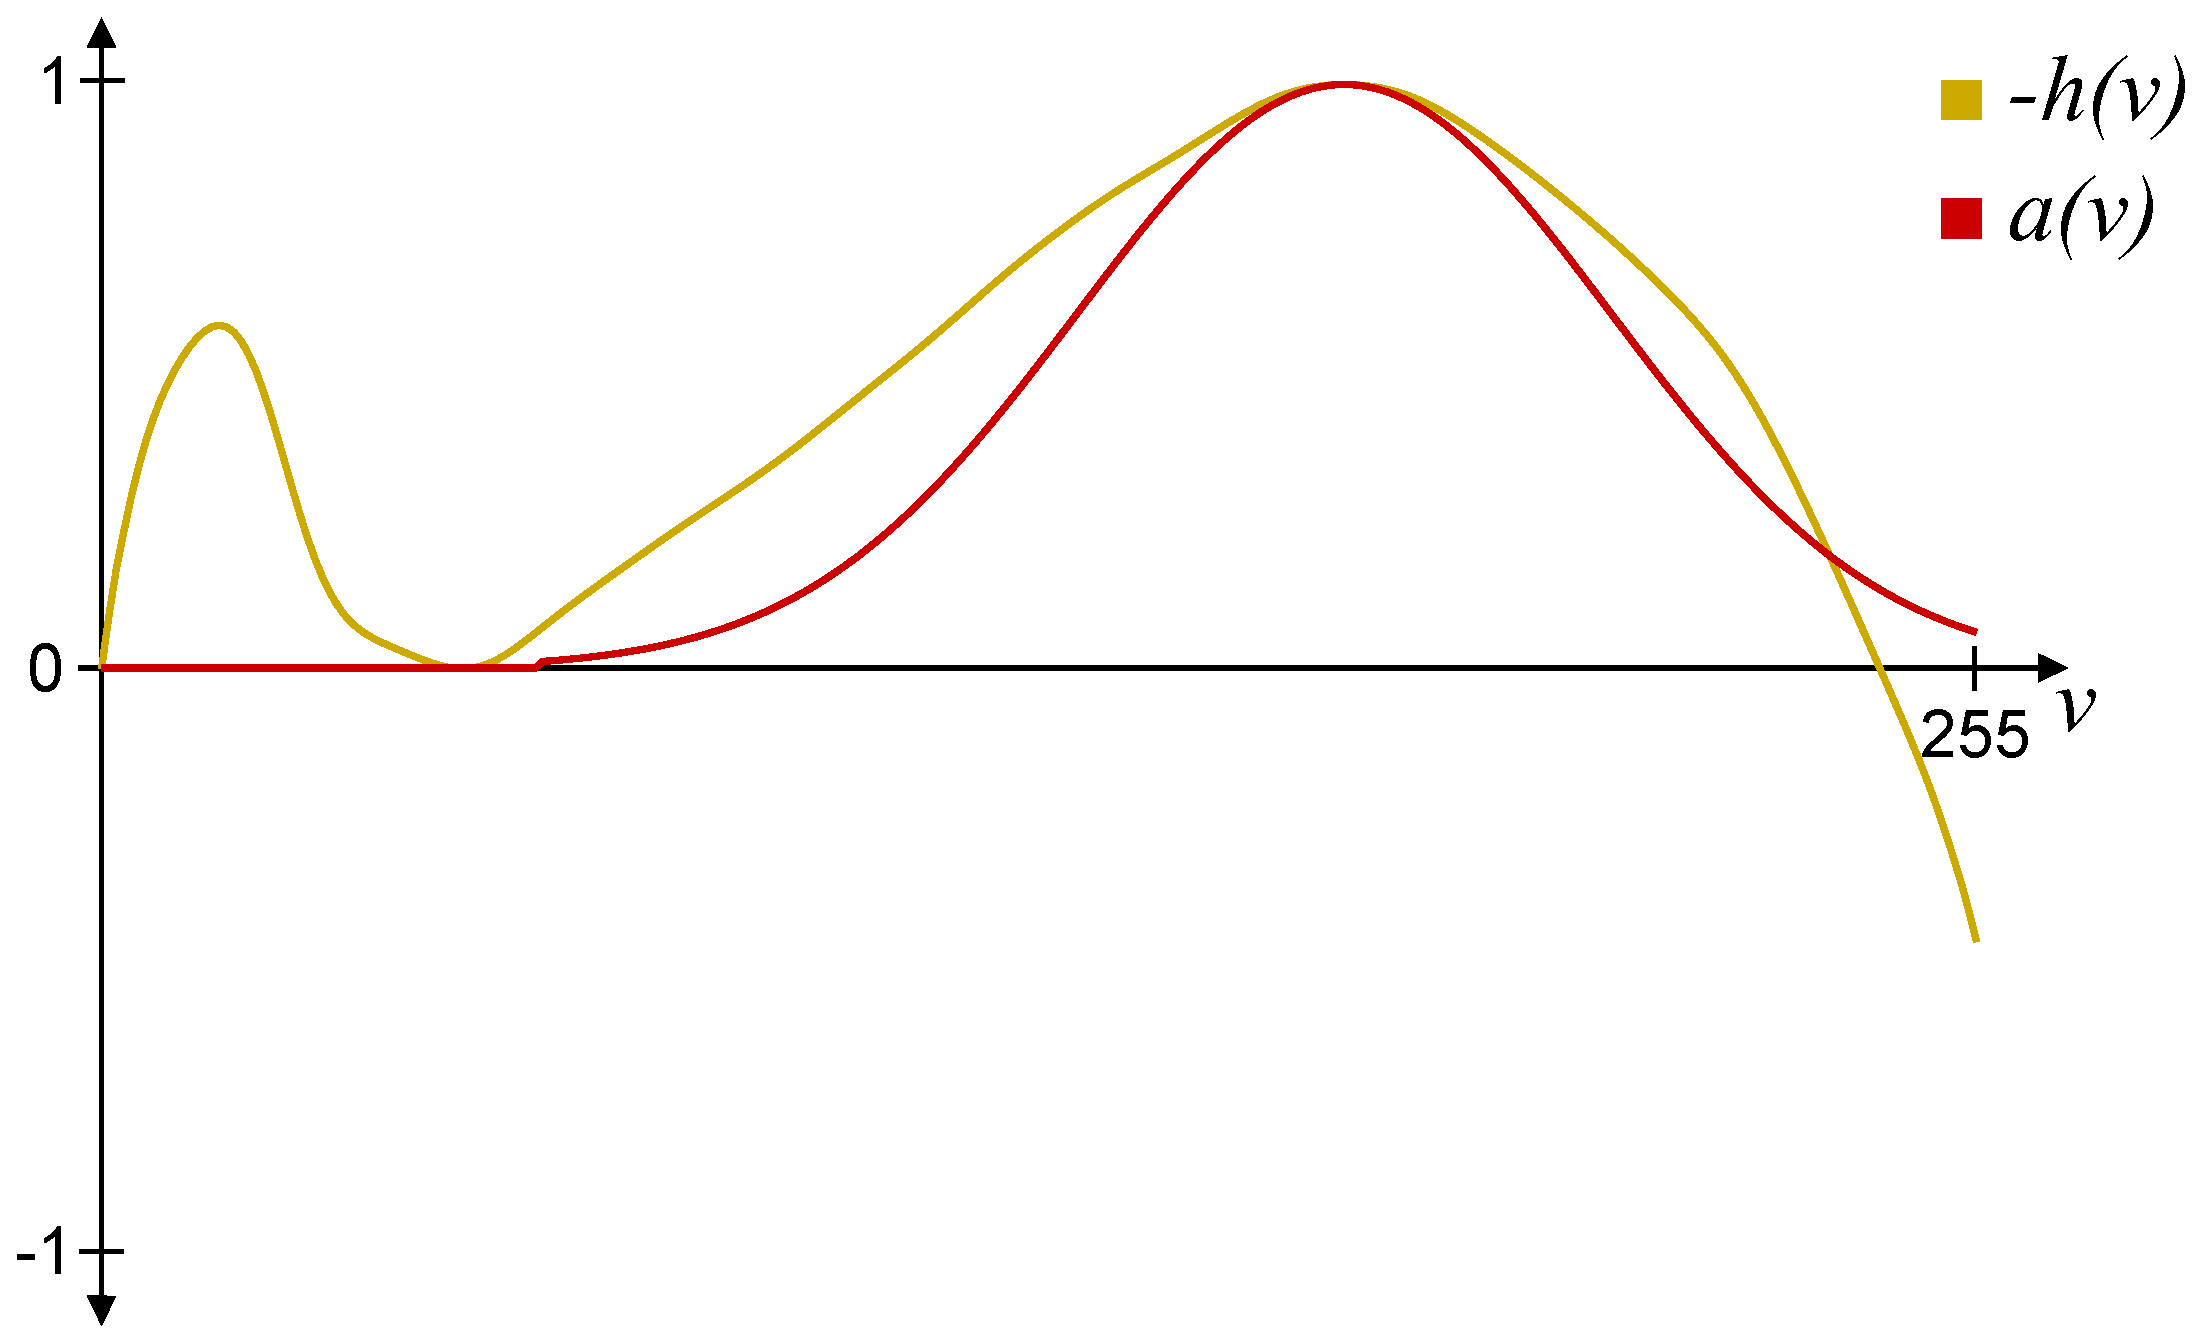
\includegraphics[width=0.7\textwidth]{images/r_m_knee_ft}
	}
	\subfigure[]
	{
		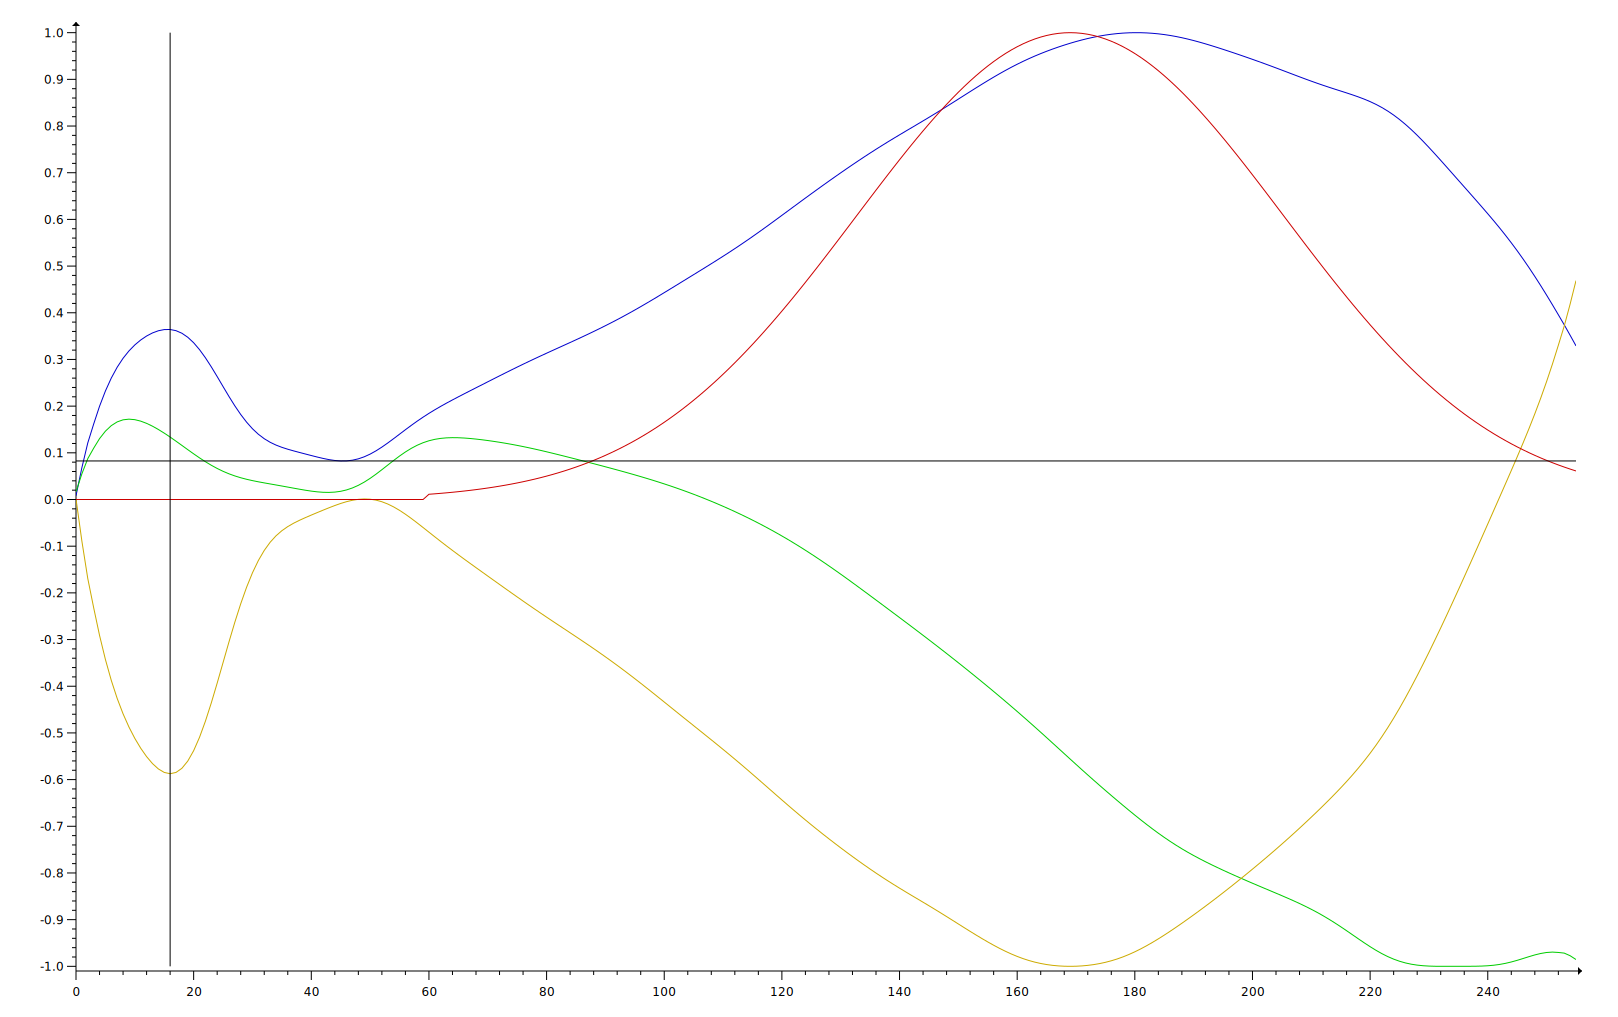
\includegraphics[width=0.7\textwidth]{images/r_m_knee}
	}
	\caption{Volume médico de joelhos.}
\end{figure}

\clearpage
\section{Malhas Não Regulares}
\label{sec:result.irreg}

	Nesta seção, são exibidos os resultados para dois modelos simples (A e B) de reservatório e um modelo real (Pituba). Para visualizar esses volumes com malhas não regulares, escolheu-se a técnica proposta por \textit{Miranda e Celes}~\cite{miranda}.
	
%%%%%%%%%%%%%%%%%%%%%%%%%%%%%%%%% VREP SO 1 %%%%%%%%%%%%%%%%%%%%%%%%%%%%%%%%%%%%
	A Figura~\ref{fig:box_slice} mostra a simulação da saturação de óleo (SO) para o modelo de reservatório A. As fronteiras fortes podem ser identificadas por regiões próximas de coloração diferente, onde suas respectivas cores não são vizinhas na escala de cores. Quanto maior a distância na escala de cores, mais forte é a fronteira. Portanto, percebe-se que este modelo possui uma fronteira forte entre o amarelo e o vermelho.\\
	
\begin{figure}[h]
	\centering
	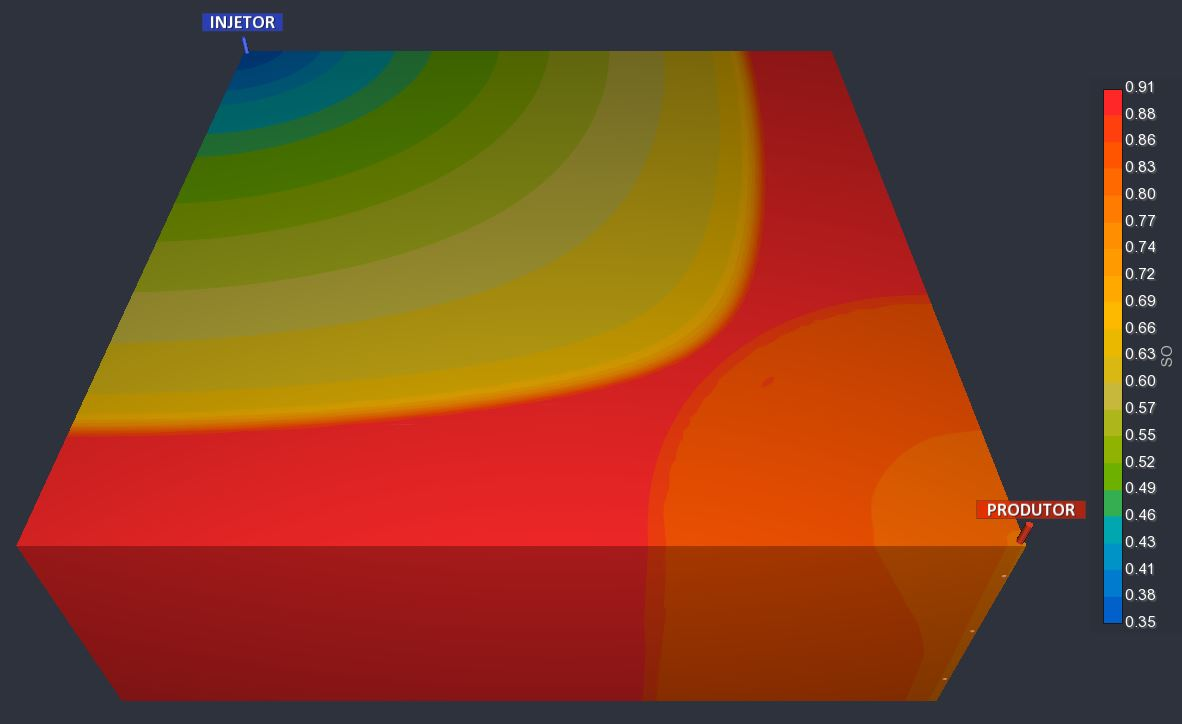
\includegraphics[width=1\textwidth]{images/r_vrep_so_slice}
	\caption{Fatia do volume de SO do modelo A.}
	\label{fig:box_slice}
\end{figure}

	A Figura~\ref{fig:r_vrep} mostra que os dois métodos identificam a fronteira mais forte. Além disso, ambos destacam também uma fronteira em azul, próximo ao posso injetor. Contudo, o método descrito por esta dissertação identifica também uma terceira fronteira, que representa a fronteira entre a região vermelha e a laranja, na Figura~\ref{fig:box_slice}. Por conta desta última fronteira, uma outra isosuperfície (em vermelho) é realçada próxima à fronteira mais forte. O mesmo ocorre com o método de \textit{Kindlmann e Durkin}, que realça uma isosuperfície pequena (semelhante a um traço) no canto inferior direito da visualização da Figura~\ref{fig:r_vrep}~\ref{fig:r_vrep_kd}
	
	Para os reservatórios é ainda mais difícil avaliar os resultados, uma vez que não se conhece as estruturas internas, como nos volumes médicos e não há \quote{ground truth}. No entanto, pode se dizer que o método proposto apresenta um resultado melhor, pois ele destaca as mesmas fronteiras que o método de \textit{Kindlmann e Durkin} e mais uma, permitindo ao usuário uma maior percepção da estrutura global do reservatório. Minimamente, indicando para o usuário onde fazer buscas.

\begin{figure}[h]
	\centering
	\subfigure[Método de \textit{Kindlmann e Durkin}.]
	{
		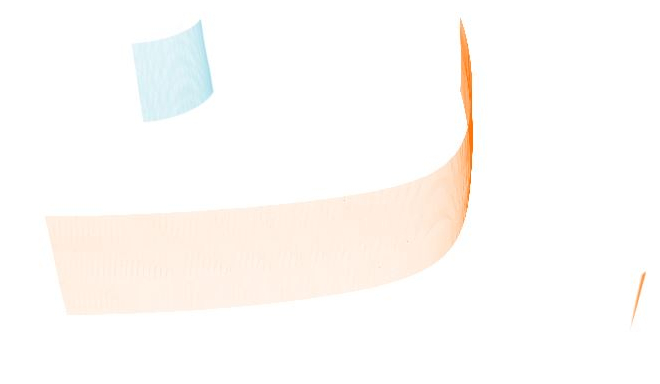
\includegraphics[width=0.35\textwidth]{images/r_vrep_so_kd}
		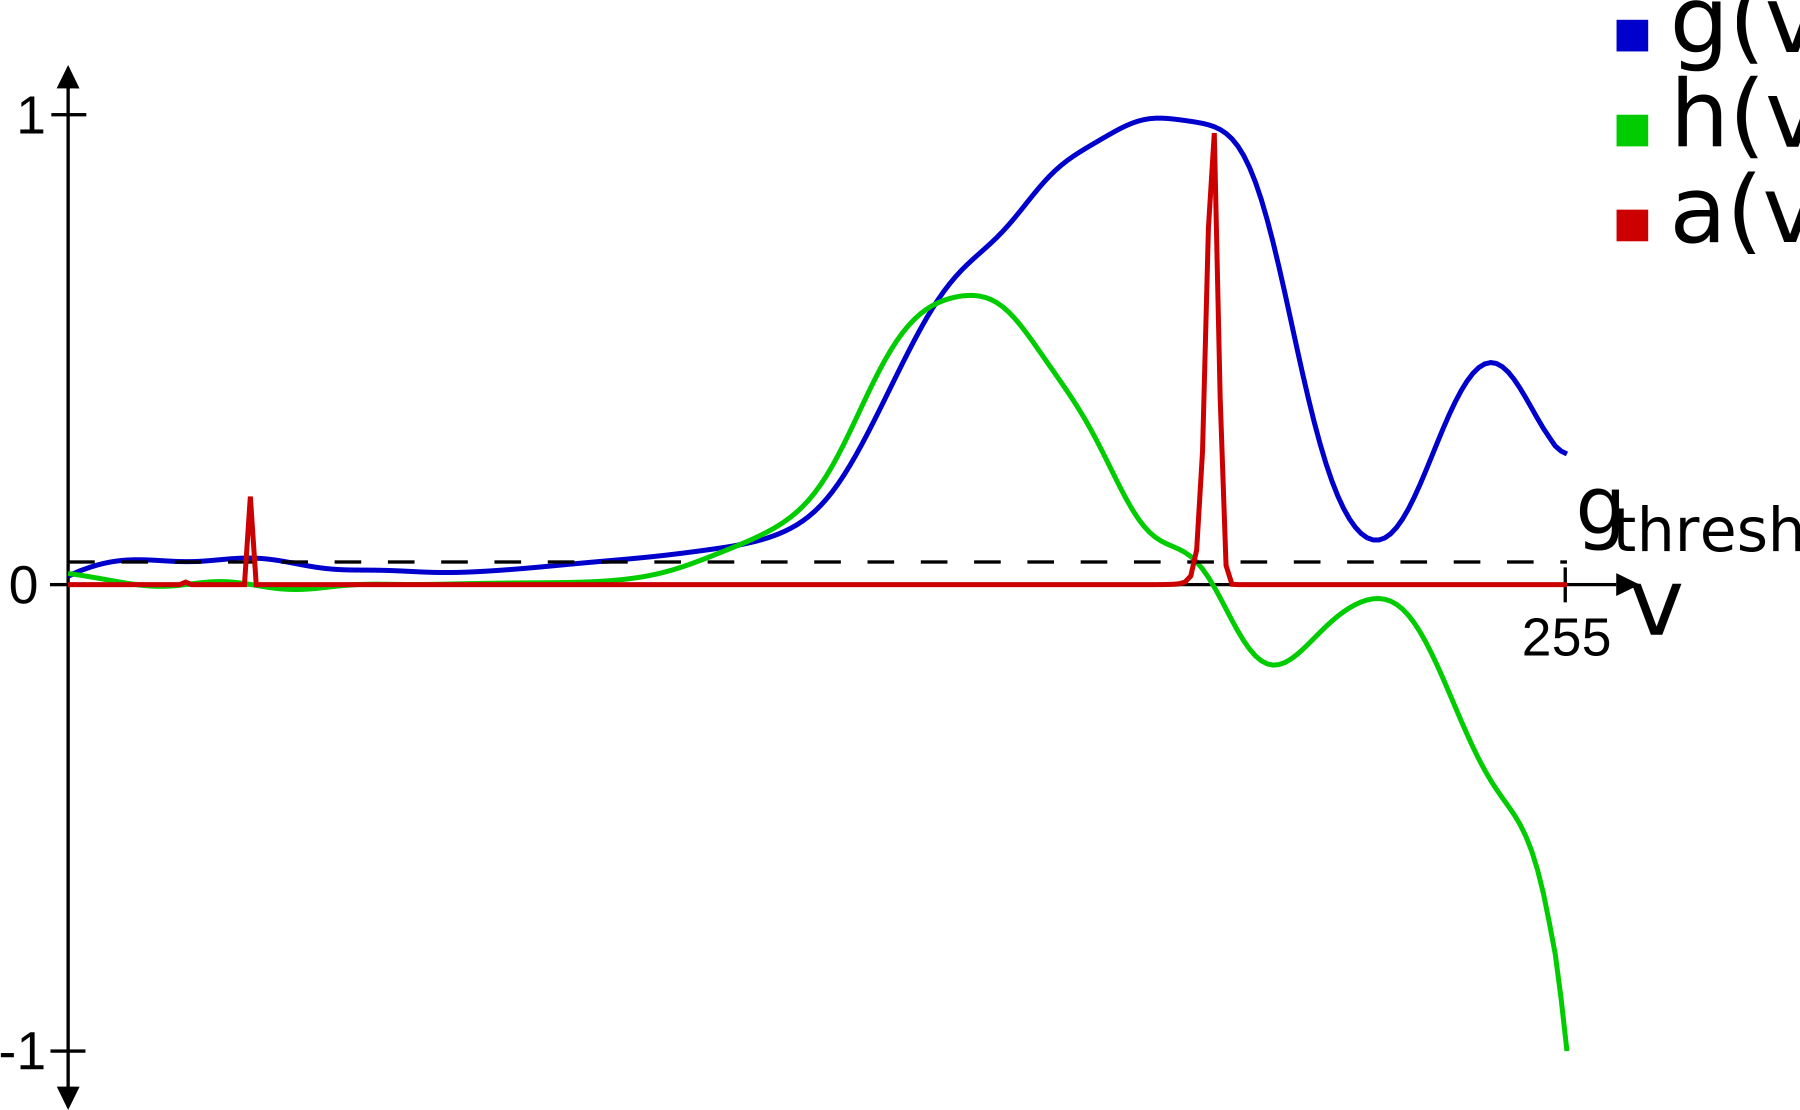
\includegraphics[width=0.65\textwidth]{images/r_vrep_so_kd_ft}
		\label{fig:r_vrep_kd}
	}
	\subfigure[Método proposto.]
	{
		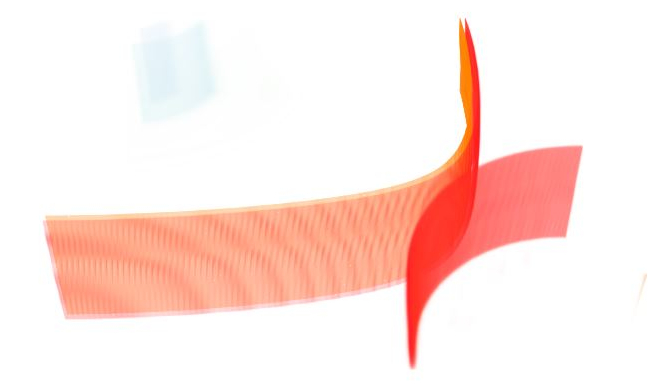
\includegraphics[width=0.35\textwidth]{images/r_vrep_so_mine}
		\includegraphics[width=0.65\textwidth]{images/r_vrep_so_mine_ft}			\label{fig:r_vrep_mine}
	}
	\caption{FT e visualização do volume de SO do modelo~A.}
	\label{fig:r_vrep}
\end{figure}

%%%%%%%%%%%%%%%%%%%%%%%%%%%%%%%%% VREP SO 2 %%%%%%%%%%%%%%%%%%%%%%%%%%%%%%%%%%%%
	A Figura~\ref{fig:r_vrep_2_slice} também exibe um volume de saturação de óleo (SO) do modelo~A, mas em outro momento da simulação. A Figura~\ref{fig:r_vrep_2} mostra que os dois métodos detectaram uma fronteira em laranja. Esta isosuperfície condiz com a evolução da área invadida esperada para este modelo, como mostra a Figura~\ref{fig:r_reserv_livro}. Apesar das fronteiras excedentes não estarem mapeadas no avanço da área invadida, percebe-se que elas realçam interfaces entres diferentes regiões do reservatório. A relevância dessas fronteiras destacadas, no entanto, precisa ser avaliada com cautela e maior conhecimento sobre reservatórios.
	
\begin{figure}[h]
	\centering
	\includegraphics[width=0.8\textwidth]{images/r_vrep_so_2_slice}
	\caption{Volume de saturação de óleo do modelo A.}
	\label{fig:r_vrep_2_slice}
\end{figure}

\begin{figure}[h]
	\centering
	\subfigure[Método de \textit{Kindlmann e Durkin}.]
	{
		\includegraphics[width=0.35\textwidth]{images/r_vrep_so_2_kd}
		\includegraphics[width=0.65\textwidth]{images/r_vrep_so_2_kd_ft}
		\label{fig:r_vrep_2_kd}
	}
	\subfigure[Método proposto.]
	{
		\includegraphics[width=0.35\textwidth]{images/r_vrep_so_2_mine}
		\includegraphics[width=0.65\textwidth]{images/r_vrep_so_2_mine_ft}			\label{fig:r_vrep_2_mine}
	}
	\caption{FT e visualização do volume de SO do modelo~A.}
	\label{fig:r_vrep_2}
\end{figure}

\begin{figure}[h]
	\centering
	\includegraphics[width=0.8\textwidth]{images/reserv_livro}
	\caption{Evolução da área invadida em uma malha de 5 pontos~\cite{rosa}.}
	\label{fig:r_reserv_livro}
\end{figure}
	
%%%%%%%%%%%%%%%%%%%%%%%%%%%%%%%%%% BOX SO %%%%%%%%%%%%%%%%%%%%%%%%%%%%%%%%%%%%%
\newpage
	A Figura~\ref{fig:r_box_so_slice} mostra a simulação da saturação de óleo para o modelo de reservatório B. Comparando-a com as visualizações das Figuras~\ref{fig:r_box_so_kd}~e~\ref{fig:r_box_so_mine}, nota-se que as isosuperfícies realçadas pelos dois métodos, são interfaces entre regiões de SO distintas. As fronteiras destacadas são diferentes e não se pode afirmar quais estão certas ou erradas. Contudo, mais uma vez o método proposto destaca uma fronteira a mais que o método de \textit{Kindlmann e Durkin}.

\begin{figure}[h]
	\centering
	\includegraphics[width=0.95\textwidth]{images/r_box_so_slice}
	\caption{Volume de saturação de óleo do modelo B.}
	\label{fig:r_box_so_slice}
\end{figure}

\begin{figure}[H]
	\centering
	\subfigure[]
	{
		\includegraphics[width=0.7\textwidth]{images/r_box_so_kd_ft}
	}
	\subfigure[]
	{
		\includegraphics[width=0.7\textwidth]{images/r_box_so_kd}
	}
	\caption{FT e visualização do volume de SO do modelo~B pelo método de \textit{Kindlmann e Durkin}.}
	\label{fig:r_box_so_kd}
\end{figure}

\begin{figure}[h]
	\centering
	\subfigure[]
	{
		\includegraphics[width=0.7\textwidth]{images/r_box_so_mine_ft}
	}
	\subfigure[]
	{
		\includegraphics[width=0.7\textwidth]{images/r_box_so_mine}
	}
	\caption{FT e visualização do volume de SO do modelo~B pelo método proposto.}
	\label{fig:r_box_so_mine}
\end{figure}

%%%%%%%%%%%%%%%%%%%%%%%%%%%%%%%%%% BOX SG %%%%%%%%%%%%%%%%%%%%%%%%%%%%%%%%%%%%%
	A Figura~\ref{fig:r_box_sg_slice} mostra a simulação da saturação de gás (SG) para o modelo de reservatório B. O método de \textit{Kindlmann e Durkin} detecta apenas uma fronteira, como pode ser visto na Figura~\ref{fig:r_box_sg_kd}. Já o método proposto nesta dissertação, destaca seis fronteiras. A menor delas realça a isosuperfície vermelha da Figura~\ref{fig:r_box_sg_mine}~\ref{fig:r_box_sg_mine_ft}, enquanto as outras realçam isosuperfícies paralelas e próximas àquela identificada pelo método de \textit{Kindlmann e Durkin}. Essas isosuperfícies estão de acordo com as interfaces entre as diferentes regiões observadas na Figura~\ref{fig:r_box_sg_slice}
	
\begin{figure}[h]
	\centering
	\includegraphics[width=1\textwidth]{images/r_box_sg_slice}
	\caption{Volume de saturação de gás do modelo B.}
	\label{fig:r_box_sg_slice}
\end{figure}

\begin{figure}[h]
	\centering
	\subfigure[]
	{
		\includegraphics[width=0.7\textwidth]{images/r_box_sg_kd_ft}
		\label{fig:r_box_sg_kd_ft}
	}
	\subfigure[]
	{
		\includegraphics[width=0.65\textwidth]{images/r_box_sg_kd}
	}
	\caption{FT e visualização do volume de SG do modelo~B pelo método de \textit{Kindlmann e Durkin}.}
	\label{fig:r_box_sg_kd}
\end{figure}

\begin{figure}[h]
	\centering
	\subfigure[]
	{
		\includegraphics[width=0.7\textwidth]{images/r_box_sg_mine_ft}
		\label{fig:r_box_sg_mine_ft}
	}
	\subfigure[]
	{
		\includegraphics[width=0.7\textwidth]{images/r_box_sg_mine}
	}
	\caption{FT e visualização do volume de SG do modelo~B pelo método proposto.}
	\label{fig:r_box_sg_mine}
\end{figure}

%%%%%%%%%%%%%%%%%%%%%%%%%%%%%%%%%% BOX SW %%%%%%%%%%%%%%%%%%%%%%%%%%%%%%%%%%%%%
\clearpage
	A Figura~\ref{fig:r_box_sw_slice} mostra a simulação da saturação de água (SW) para o reservatório B. Esse modelo exemplifica bem a diferença entre os dois métodos quanto ao número de fronteiras, pois, assim como no modelo anterior, o método de \textit{Kindlmann e Durkin} detecta apenas uma fronteira, que pode ser vista na Figura~\ref{fig:r_box_sw_kd}.
	
	No entanto, o método de \textit{Kindlmann e Durkin} não é capaz de realçar a fronteira existente entre as regiões vermelha e amarela. Observando a escala de cores, na Figura~\ref{fig:r_box_sw_slice}, vê-se que a fronteira não detectada possui a mesma importância que a detectada, pois o range de valores que estas abrangem é similar. A fronteira faltante na detecção do método de \textit{Kindlmann e Durkin} é corretamente destacada pelo método proposto nesta dissertação. Na~Figura~\ref{fig:r_box_sw_mine} vê-se a isosuperfície esperada no formato de um cone vermelho. O método proposto destaca também a mesma fronteira encontrada por \textit{Kindlmann e Durkin}, além de quatro outras intermediárias.
	
\begin{figure}[h]
	\centering
	\includegraphics[width=1\textwidth]{images/r_box_sw_slice}
	\caption{Volume de saturação de água do modelo B.}
	\label{fig:r_box_sw_slice}
\end{figure}

\begin{figure}[h]
	\centering
	\subfigure[]
	{
		\includegraphics[width=0.7\textwidth]{images/r_box_sw_kd_ft}
		\label{fig:r_box_sw_kd_ft}
	}
	\subfigure[]
	{
		\includegraphics[width=0.7\textwidth]{images/r_box_sw_kd}
	}
	\caption{FT e visualização do volume de SW do modelo~B pelo método de \textit{Kindlmann e Durkin}.}
	\label{fig:r_box_sw_kd}
\end{figure}

\begin{figure}[h]
	\centering
	\subfigure[]
	{
		\includegraphics[width=0.7\textwidth]{images/r_box_sw_mine_ft}
	}
	\subfigure[]
	{
		\includegraphics[width=0.7\textwidth]{images/r_box_sw_mine}
	}
	\caption{FT e visualização do volume de SW do modelo~B pelo método proposto.}
	\label{fig:r_box_sw_mine}
\end{figure}

	Assim, percebe-se que o método proposto por esta dissertação, realça mais interfaces entre regiões de diferentes intensidades, revelando ao usuário (de forma automática), uma estrutura global do dado volumétrico sendo visualizado.

%%%%%%%%%%%%%%%%%%%%%%%%%%%%%%%%%% Pituba %%%%%%%%%%%%%%%%%%%%%%%%%%%%%%%%%%%%%
\clearpage
	A Figura~\ref{fig:r_pituba} mostra um momento da simulação da saturação de óleo de um modelo real de reservatório de petróleo, o Pituba. Essa visualização, feita pelo Geresim, incorpora uma função de transferência gerada automaticamente pelo método proposto nesta dissertação. Para este caso, não gerou-se uma função de opacidade mas uma função de peso, isto é, o valor da FT gerada multiplica cada coordenada rgb da FT de cores do Geresim. Assim, as fronteiras são realçadas através de cores mais claras, enquanto todo o resto do modelo possui tonalidades mais escuras.
	
\begin{figure}[h]
	\centering
	\includegraphics[width=1\textwidth]{images/pituba}
	\caption{Visualização do modelo Pituba através do Geresim, com uma FT gerada automaticamente pelo método descrito nesta dissertação.}
	\label{fig:r_pituba}
\end{figure}
	
	Nesta figura observa-se fronteiras (de cor laranja) circundando os poços de injeção (em azul). Essas regiões são consistentes com as fronteiras de avanço esperadas, já que é a partir dos poços de injeção de água que se formaram as interfaces entre a água e o óleo e, portanto, obtém a maior variação na saturação de óleo. Sendo assim, as fronteiras identificadas são bons indícios de onde se encontram as frentes de avanço.